\chapter{Deanonymization of cryptocurrency transactions with network analysis} % Main chapter title

\label{Chapter03Clustering}

In this Chapter, we tackle the following question: can a global passive adversary.infer relationships between transactions based solely on their propagation pattern in the network?
We review the Bitcoin's P2P protocol and propose an algorithm that allows us to distinguish transactions issued from the same node from transactions issued from different nodes (with s certain degree of accuracy).
We implement and test our method on Bitcoin and three other cryptocurrencies focused on privacy: Dash, Monero, and Zcash.
We also test the same technique on transactions issued from mobile wallets, which are studied in more detail in the subsequent chapter.

We present a novel technique to analyze the public traffic in a P2P network of Bitcoin and other cryptocurrencies and extract information about the senders of transactions.

Previous work in cryptocurrency privacy mostly focused on applying data mining algorithms to the transaction graph extracted from the blockchain.
We focus on a less well researched vector for privacy attacks: network analysis.
We analyze propagation times of protocol messages to infer relationships between transactions.
We argue that timings of transaction messages leak information about their origin, which can be exploited by a well connected adversarial node.
For the first time, network level attacks on Bitcoin and the three major privacy-focused cryptocurrencies have been examined.
We describe the message propagation mechanics and privacy guarantees in Bitcoin, Dash, Monero, and Zcash.
We propose a novel technique for linking transactions based on transaction propagation analysis.
We also unpack address advertisement messages (\texttt{ADDR}), which under certain assumptions may help in linking transaction clusters to IP addresses of nodes.
We implement and evaluate our method, deanonymizing our own transactions in Bitcoin and Zcash with a high level of accuracy.
We also show that our technique is applicable to Dash and Monero.
We estimate the cost of a full-scale attack on the Bitcoin mainnet at hundreds of US dollars, feasible even for a low budget adversary.

The ultimate goal of deanonymization is to reveal the relationship between cryptocurrency transactions (or addresses) and real-world identifiers, such as IP addresses.
In our model, the goal of the adversary in our model is to infer a connection between a cryptocurrency transaction and the IP address of a node which was the first to introduce it into the network.\footnote{Even though an IP address is not linked to a physical person, it can be used to determine a relatively precise location of the device involved, and can be linked to a real-world identity if the responsible ISP is compromised.}
We rely on the core observation that a node can be uniquely identified by its set of connected peers (\textit{entry nodes}).
Earlier network-based deanonymization attacks~\cite{Biryukov2014, Koshy2014} only took into account the first node to propagate a given transaction to the adversary.
Our approach is more sophisticated.
We apply carefully chosen weight functions to message timing information.
This allows us to link transactions broadcast from one node, even if all addresses involved are unrelated (consequently, blockchain analysis would gain no insight).

Instead of associating transactions with IP addresses directly, we first cluster the transactions, and then try to assign IP addresses to clusters.
Even if the latter step gains no insight, the clustering data used in combination with information from other sources is useful for the attacker.
Moreover, our technique does not simply produce a binary decision (whether two transactions are related), but also allows for manual visual inspection of transaction clusters using heatmaps.

We now provide the background on message propagation in Bitcoin and other cryptocurrencies, and present our approach to transaction clustering based on propagation timing.
We implement and evaluate our technique on real-world cryptocurrencies.
We were able to cluster our own transactions in Bitcoin and Zcash with high levels of precision and recall.
In particular, in the case of Zcash, we can cluster transactions involving both transparent and shielded addresses.
We also show that our technique is applicable to Dash and Monero.
We provide rough calculations of the necessary resources and the monetary cost of an attack on the Bitcoin mainnet.
We discuss attack scenarios for different types of wallets, and give a number of recommendations for users who want to preserve their privacy, as well as for developers of cryptocurrency protocols and wallets who want to give users an easier way to do so.

This Chapter is based on~\cite{Biryukov2019a} and~\cite{Biryukov2019b}.

\section{Transaction clustering with timing analysis}  \label{sec:Ch03Ourapproach}

\subsection{Algorithm overview}

Our goal is to cluster transactions based on the node which was the first to introduce them into the network.
Consider the first $N$ nodes which relayed a transaction to our listening node.
We assign weights to IP addresses of nodes depending on the propagation timestamps.
Intuitively, a peer that relays a new transaction to us quickly is likely to be an entry node or closely connected to one.
Our clustering algorithm is based on the weight vectors of transactions.
We expect transactions originating from one node to yield relatively well-correlated weight vectors.

Due to broadcast randomization, we do not expect all transactions from one node to be well-correlated.
But the matrix of pairwise correlations exhibits special behavior which would help us infer transactions clusters nevertheless.
Consider a node with eight entry nodes with IP addresses ($p_1$ to $p_8$) making three transactions: $tx_1, tx_2, tx_3$.
If transactions were broadcast in batch via the same subset of the entry nodes, their weight vectors would be very similar.
But due to diffusion or trickling, the following scenario is more typical: $tx_1$ quickly relayed from $p_{\{1,2,3\}}$, $tx_2$ from $p_{\{3,4,5\}}$, $tx_3$ from $p_{\{5,6,7\}}$.
If we considered only the first propagation, these transactions would seem completely unrelated.
But with weight vectors, considering that those are sparse, the correlation between $tx_1$ and $tx_2$ and between $tx_2$ and $tx_3$ would be noticeable, which would allow us to reveal not only the relationship between these pairs but also among all three transactions.
Note that this technique is also applicable for transactions originating from a light client (in this case, a cluster represents transactions from multiple clients connected to the same full node).

\subsection{Weight functions and clustering}

Let $tx$ be a transaction.
Let $p^{tx} = [p^{tx}_1, p^{tx}_2, ... p^{tx}_N]$ be the vector of the first $N$ IP addresses which relayed $tx$ to us.
Let $t^{tx} = [t^{tx}_1, t^{tx}_2, ... t^{tx}_N]$ be the vector of the corresponding \textit{relative} timestamps.
A \textit{relative} timestamp is defined as $t = t^{abs}_i - t^{abs}_0$, where $t_{abs}^i$ is the absolute time time (UNIX timestamp) when we received transaction $tx_i$ (i.e.,~we subtract the timestamp of the first propagation of this transaction from all its propagations).
For each $p^{tx}_i \in p^{tx}$, we assign a parameterized weight as follows:

\[
w_k(p^{tx}_i) = e^{-(t^{tx}_i/k)^2}
\]

The weight function is chosen to reflect the decreasing importance of every next broadcast.
$p_1$ is assigned the maximal weight of $1.0$ (note that $t_1=0$ by definition); other nodes receive lower weights.
Our experiments show that this function family yields better clustering (compared to $1/(kt)$ and $e^{-kt}$).
The intuition is that it gives higher weights to a certain window depending on $k$ while exponentially decreasing outside of it.
Moreover, window size is adjusted for each vector.

For each $p^{tx}$, we want to use such $w_k$ that gives sufficient variance among the weight values.
Weights quickly fall to nearly zero if $k$ is too low and stay close to one if $k$ is high.
Let $t^{tx}_{med}$ be the median value in $t^{tx}$ (average of the high and low medians if the length of $t^{tx}$ is even).
We choose $k^{tx}_{opt}$ s.t.~the weight of $t^{tx}_{med}$ would be $0.5$:

\[
k^{tx}_{opt} = \frac{t^{tx}_{med}}{\sqrt{-\ln(0.5)}}
\]

This choice of $k$ distributes the weights for any $t^{tx}$: they neither stay close to one nor quickly fall to zero (see examples in Figure~\ref{fig:weight}).
\begin{figure}
	\centering
	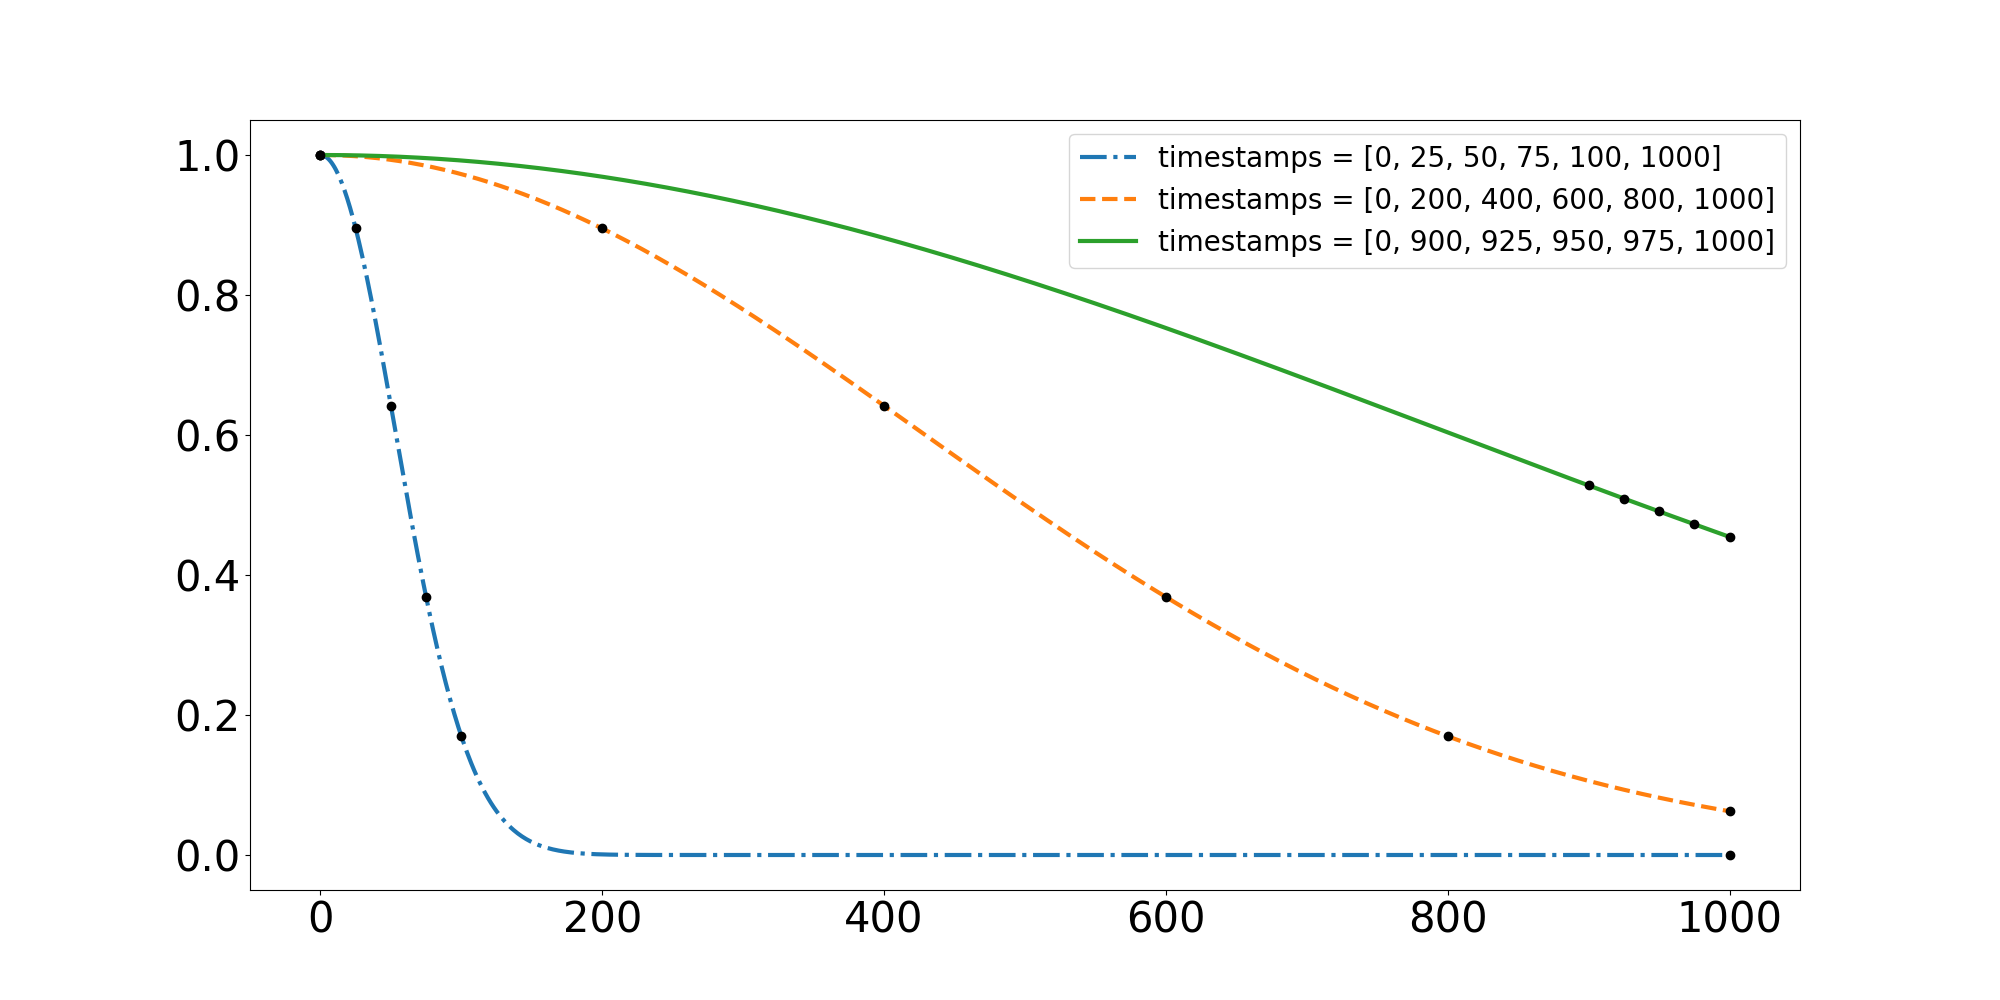
\includegraphics[width=\columnwidth]{weight-function-example.png}
	\caption{Weight functions for three timestamp vectors}\label{fig:weight}
\end{figure}
For each transaction, we evaluate the vector of weights:

\[
w^{tx} = w_{k^{tx}_{opt}}(t^{tx})
\]

Let $X$ be the set of all transactions we consider.
Let $P$ be the set of IP addresses of nodes which appeared in at least one of $p$ vectors in $X$:

\[
P = \bigcup\limits_{tx \in X} p^{tx}
\]

We define an extended weight vector $v_{tx}$ for each $tx$ by setting the weight of nodes in $P \backslash p^{tx}$ to zero and sort the values in the weight vectors w.~r.~t.~the alphabetical order of $P$.
We then calculate a matrix where an element in $i$-th row and $j$-th column is the Pearson correlation of the extended weight vectors $v_{tx_i}$ and $v_{tx_j}$.
This matrix can supposedly be transformed into a block-diagonal matrix with blocks (clusters) corresponding to transaction sources.

To reveal the clusters, we use spectral co-clustering~\cite{Dhillon2001} implemented in the Python \texttt{sklearn.cluster.bicluster} module~\cite{scikitlearn2018}.
Given an input matrix $A$, the algorithm preprocesses it as follows:

\[
A_n = R^{1/2}AC^{-1/2}
\]

Where $R$ is the diagonal matrix with entry $i$ equal to $\sum_{j} A_{ij}$, and $C$ is the diagonal matrix with entry $j$ equal to $\sum_{i} A_{ij}$.

The singular value decomposition of $A$ provides the partitions of rows and columns: $A_{n}=U \Sigma V^{T}$.
The $l$ = $\lceil \log_2 k \rceil$ singular vectors provide the partitioning information.
Let $U$ be a matrix with columns $u_2,\dots,u_{l+1}$, and similarly for $V$.
Then $Z$ is defined as:

\[
Z = 
\begin{bmatrix}
R^{-1/2} & U \\
C^{-1/2} & V
\end{bmatrix}
\]

The rows of $Z$ are clustered using the k-means algorithm.


\subsection{Measuring clustering quality}

We use the Rand score as an external metric of clustering quality, as described in~\cite{Amigo2009} (Section~4.2).
The Rand score operates on \textit{pairs} of elements and reflects the proportion of "right decisions" regarding whether to put a pair of transactions into one or different clusters.

$SS$, $SD$, $DS$, and $DD$ are numbers of transaction pairs defined as follows:
\begin{itemize}
	\item SS: same cluster, same category (two of our transactions in the same cluster);\footnote{In our case, there are only two categories: "our" and "foreign" transactions.}
	\item SD: same cluster, different category (our and foreign transactions in the same cluster);
	\item DS: different cluster, same category (two of our transactions in different clusters);
	\item DD: different cluster, different category (our and foreign transactions in different clusters).
\end{itemize}

Note that this assessment only considers clusters with "our" transactions, because we do not know whether any two "foreign" transactions should have been assigned to the same cluster:

\[
R = \frac{SS + DD}{SS + SD + DS + DD}
\]

We further modify this metric by parameterizing it with the minimal number of our transactions in a cluster required to consider it in the calculation.
In our experiments, we only consider clusters with at least two of our transactions.
With no such threshold, large clusters with one of our transactions disproportionately increase $DD$ and bring the score close to 1.0, which does not reflect the subjective amount of information an adversary acquires.

\subsubsection{Measuring the degree of deanonymization}

To estimate the success rate of the attack, we use a quality score based on the \textit{anonymity degree} proposed by D{\'{\i}}az et al.~\cite{Diaz2002}.
The anonymity degree is designed to measure the amount of information an attacker gains compared to perfect anonymity (where each user has an equal probability of being the originator of a given message).
Let $p_i$ be the probability that a transaction $i$ originates from a given source $S_{control}$; $N$ is the total number of transactions.
The entropy is calculated as:

\[
H(X) = -\sum_{i=1}^N p_i log_2(p_i)
\]

The maximal entropy is:
\[
H_M = log_2(N)
\]

The anonymity degree is defined as:

\[
d = \frac{H(X)}{H_M}
\]

The anonymity degree does not reflect the fact that the probability distribution obtained by the adversary may not be well aligned with the true probability distribution.
To address this issue, we propose an \textit{adjusted} anonymity degree.
First, we calculate the median square error $e$ between our probability distribution and the known true distribution (1 for transactions from $S_{control}$ and 0 for others), based on a subset of transactions from the control set.
The adjusted anonymity degree is defined as follows:

\[
d_{adj} = 1 - (1 - e) * (1 - d)
\]

To explain on two edge case examples: If $e = 0$ (the attacker precisely predicted the distribution), $d_{adj} = d$; if $e = 1$ (the attacker's distribution does not at all reflect the reality), $d_{adj} = 1$ (the system retains full anonymity).

The assumptions of our model have their limitations.
Our clustering technique depends on a user issuing a series of transactions in a relatively short time window of several minutes (up to an hour), through the same set of entry nodes (i.e. from the same session).
If a user re-launches the client, their transactions issued before and after this event would not be linkable by our technique.
%While this scenario may not be prevalent, it may gain popularity in the future, as cryptocurrencies gain broader adoption and at least partially solve the scalability issues.


\section{Implementation details}

We use a modified Bitcoin network probing tool \texttt{bcclient}~\cite{Pustogarov2017} to maintain parallel connections to peers and log incoming messages: transaction hash, the IP which relayed it to us, and the timestamp of this event.

To adapt \texttt{bcclient} for usage with Dash and Zcash, we change the relevant constants (port numbers, protocol magic bytes, DNS seeder addresses).
For Monero, which is not a Bitcoin fork, we modified the full node reference implementation (\texttt{monerod}), adding the required logging and disabling the built-in limits on the total bandwidth as well as artificial delays between network requests.

For the purposes of clustering, we only log \texttt{INV} messages, and never continue with the \texttt{GETDATA} -- \texttt{TX} exchange.
For some experiments, we also log \texttt{ADDR} messages to infer the set of most probable IP addresses corresponding to each cluster (only on the Bitcoin testnet).
For clarity, when describing our data analysis, we will refer to transaction inventory messages as "transactions".

We use Python scripts to extract the essential information from the log, save it in a more compact JSON format, analyze the data, and visualize the results.
For each transaction, we save a list of \textit{(t, IP)} pairs, where $t$ is a \textit{relative} timestamp.

\section{Experimental evaluation}

\subsection{Experiment overview}

Assume our goal is to cluster transactions originating from one target source $S_{control}$.
We capture $N$ transactions and know that $n$ of them were issued from $S_{control}$; $k$ of them are known to us.
For each transaction $i$, we assign an a priori probability of having originated from $S_{control}$: $p_i = n / N$.
The outline of our experiment is as follows.

\begin{enumerate}
	\item collect a fresh list of live network peers;
	\item establish a number of parallel connections to them, log the timestamps of receiving \texttt{INV} and \texttt{ADDR} messages;
	\item launch two nodes $S_{learn}$ and $S_{control}$, so that their initial \texttt{ADDR} advertisements would be logged;
	\item issue two series of transactions (the learning and the control sets) from $S_{learn}$ and $S_{control}$ respectively;
	\item for each considered number of first propagations, calculate the transaction correlation matrix;
	\item run the clustering algorithm with various assumed average number of transactions per cluster;
	\item choose the best clustering by Rand score on the "learning" set;
	\item in the best clustering, assign the cluster weights proportionally to the distribution of $k$ known transactions from $S_{control}$;
	\item assign zero probability of being in $S_{control}$ to transactions from $S_{learn}$;
	\item re-distribute the probability weight among transactions in each cluster;
	\item calculate the final adjusted anonymity score;
	\item re-arrange the clusters such that large correlations would be close to the diagonal (closely correlated clusters should be close in the picture);
	\item visualize the results as a heatmap.
\end{enumerate}

We use heatmaps to visualize the results.
A heatmap is a matrix where each row and each column represents a transaction that we captured during an experiment.
The color of the square at the intersection of the $k$-th row and $n$-th column represent the correlation of weight vectors of $k$-th and $n$-th transactions (darker is higher).
Note the the heatmap is diagonally symmetric by definition (black squares along the  main diagonal reflect the fact that a transaction has a $1.0$ correlation with itself).

Our assumption is that there exist a permutation of rows and columns such that the highly correlated elements would be close to the main diagonal and would exhibit a block-diagonal structure, revealing possible relations between transactions issued from the same node.
In the figures below, ticks along the axes indicate our transaction from the control set.


\subsection{Results for desktop wallets}

We evaluate our method by clustering our own transactions in Bitcoin (testnet and mainnet) and Zcash.
For these experiments, we log the traffic (both \texttt{INV} and \texttt{ADDR} messages) for 15~minutes.
The anonymity degree calculated on our own transactions indicates a substantial loss of privacy.
For Dash and Monero, we ran the clustering algorithm without calculating an external quality metric.
We obtained clearly visible clusters, which indicated that our approach is applicable for these cryptocurrencies as well.

All linkage experiments were done on our own transactions and when possible on the testnets.
The experiments on the Bitcoin mainnet deliberately did not attempt to occupy all connection slots, and operated only on a subset of 1000~nodes (out of approximately 10\,000).

% California: experiment-1541509693
% Tokyo: experiment-1541511845
% Frankfurt: experiment-1541513977
% 3-experiment: experiment-1541516997
\begin{table*}[!t]
	\normalsize
	\caption{Experiments on Bitcoin testnet and Zcash. The * sign indicates results obtained in experiments where we only connected to a subset of network nodes.}
	\centering
	\begin{tabular}{ | l | l | c | c | c | c | c | }
		\hline
		Network & Listener location & Anon. degree & Servers & Avg free slots & Tx INVs & ADDRs \\
		\hline
		Bitcoin test & California & 0.83 & 1141 & 64 & 139 & 402 \\
		Bitcoin test & Tokyo & 0.80 & 1128 & 64 & 193 & 414 \\
		Bitcoin test & Frankfurt & 0.72 & 1137 & 64 & 172 & 403 \\
		Bitcoin test & combined & 0.63 & 1154 & 63 & 250 & 1321 \\
		Bitcoin main & Frankfurt & 0.88 & 1000* & 25* & 3238 & 11300 \\
		Zcash & Frankfurt & 0.86 & 206 & 36 & 62 & 1086 \\
		\hline
	\end{tabular}
	\label{tab:results}
\end{table*}

\subsubsection{Bitcoin testnet}

We performed four experiments on the Bitcoin testnet.
For all experiments, our listening node attempted to occupy up to 117 slots for all servers.
We performed three independent experiments for three listener locations and a fourth experiment where we use all three servers simultaneously: we divide the fresh list of live peers into three equal parts, distribute them among the three servers, and then merge the three log files.
The goal of the fourth experiment was to measure the advantage an adversary may gain from using geographically distributed servers.
As listening nodes, we used Amazon EC2 servers in three geographical locations: Frankfurt (Germany), Tokyo (Japan), and North California (the US).
In all experiments, test transactions were issued from computers located in Europe.

We issued two sets of test transactions (the learning and the control sets) containing 30~transactions each.
We denote 10~transactions out of the control set as "known" to estimate the anonymity degree.

Note that the number of live peers collected by each of the listeners is very close, which indicates that we do obtain a complete view of the network.
Note also that the number of received transactions varies little between experiments, whereas the number of \texttt{ADDR} messages is significantly higher in the experiment with three listeners.
This confirms our hypothesis that address advertisements propagate through the network more slowly than transactions and blocks.
The number of average available slots is independent of the location of the listener.
The anonymity degree is lower (i.e.,~better for the attacker) in the Frankfurt experiment, which may be explained by the fact that the nodes issuing test transactions were closer to the listening nodes than in the other experiments.
The joint experiments which combined information from three geographically distributed listeners gained the best results with an anonymity degree of 0.63.

\begin{figure*}
	\centering
	\begin{minipage}{0.5\textwidth}
		\centering
		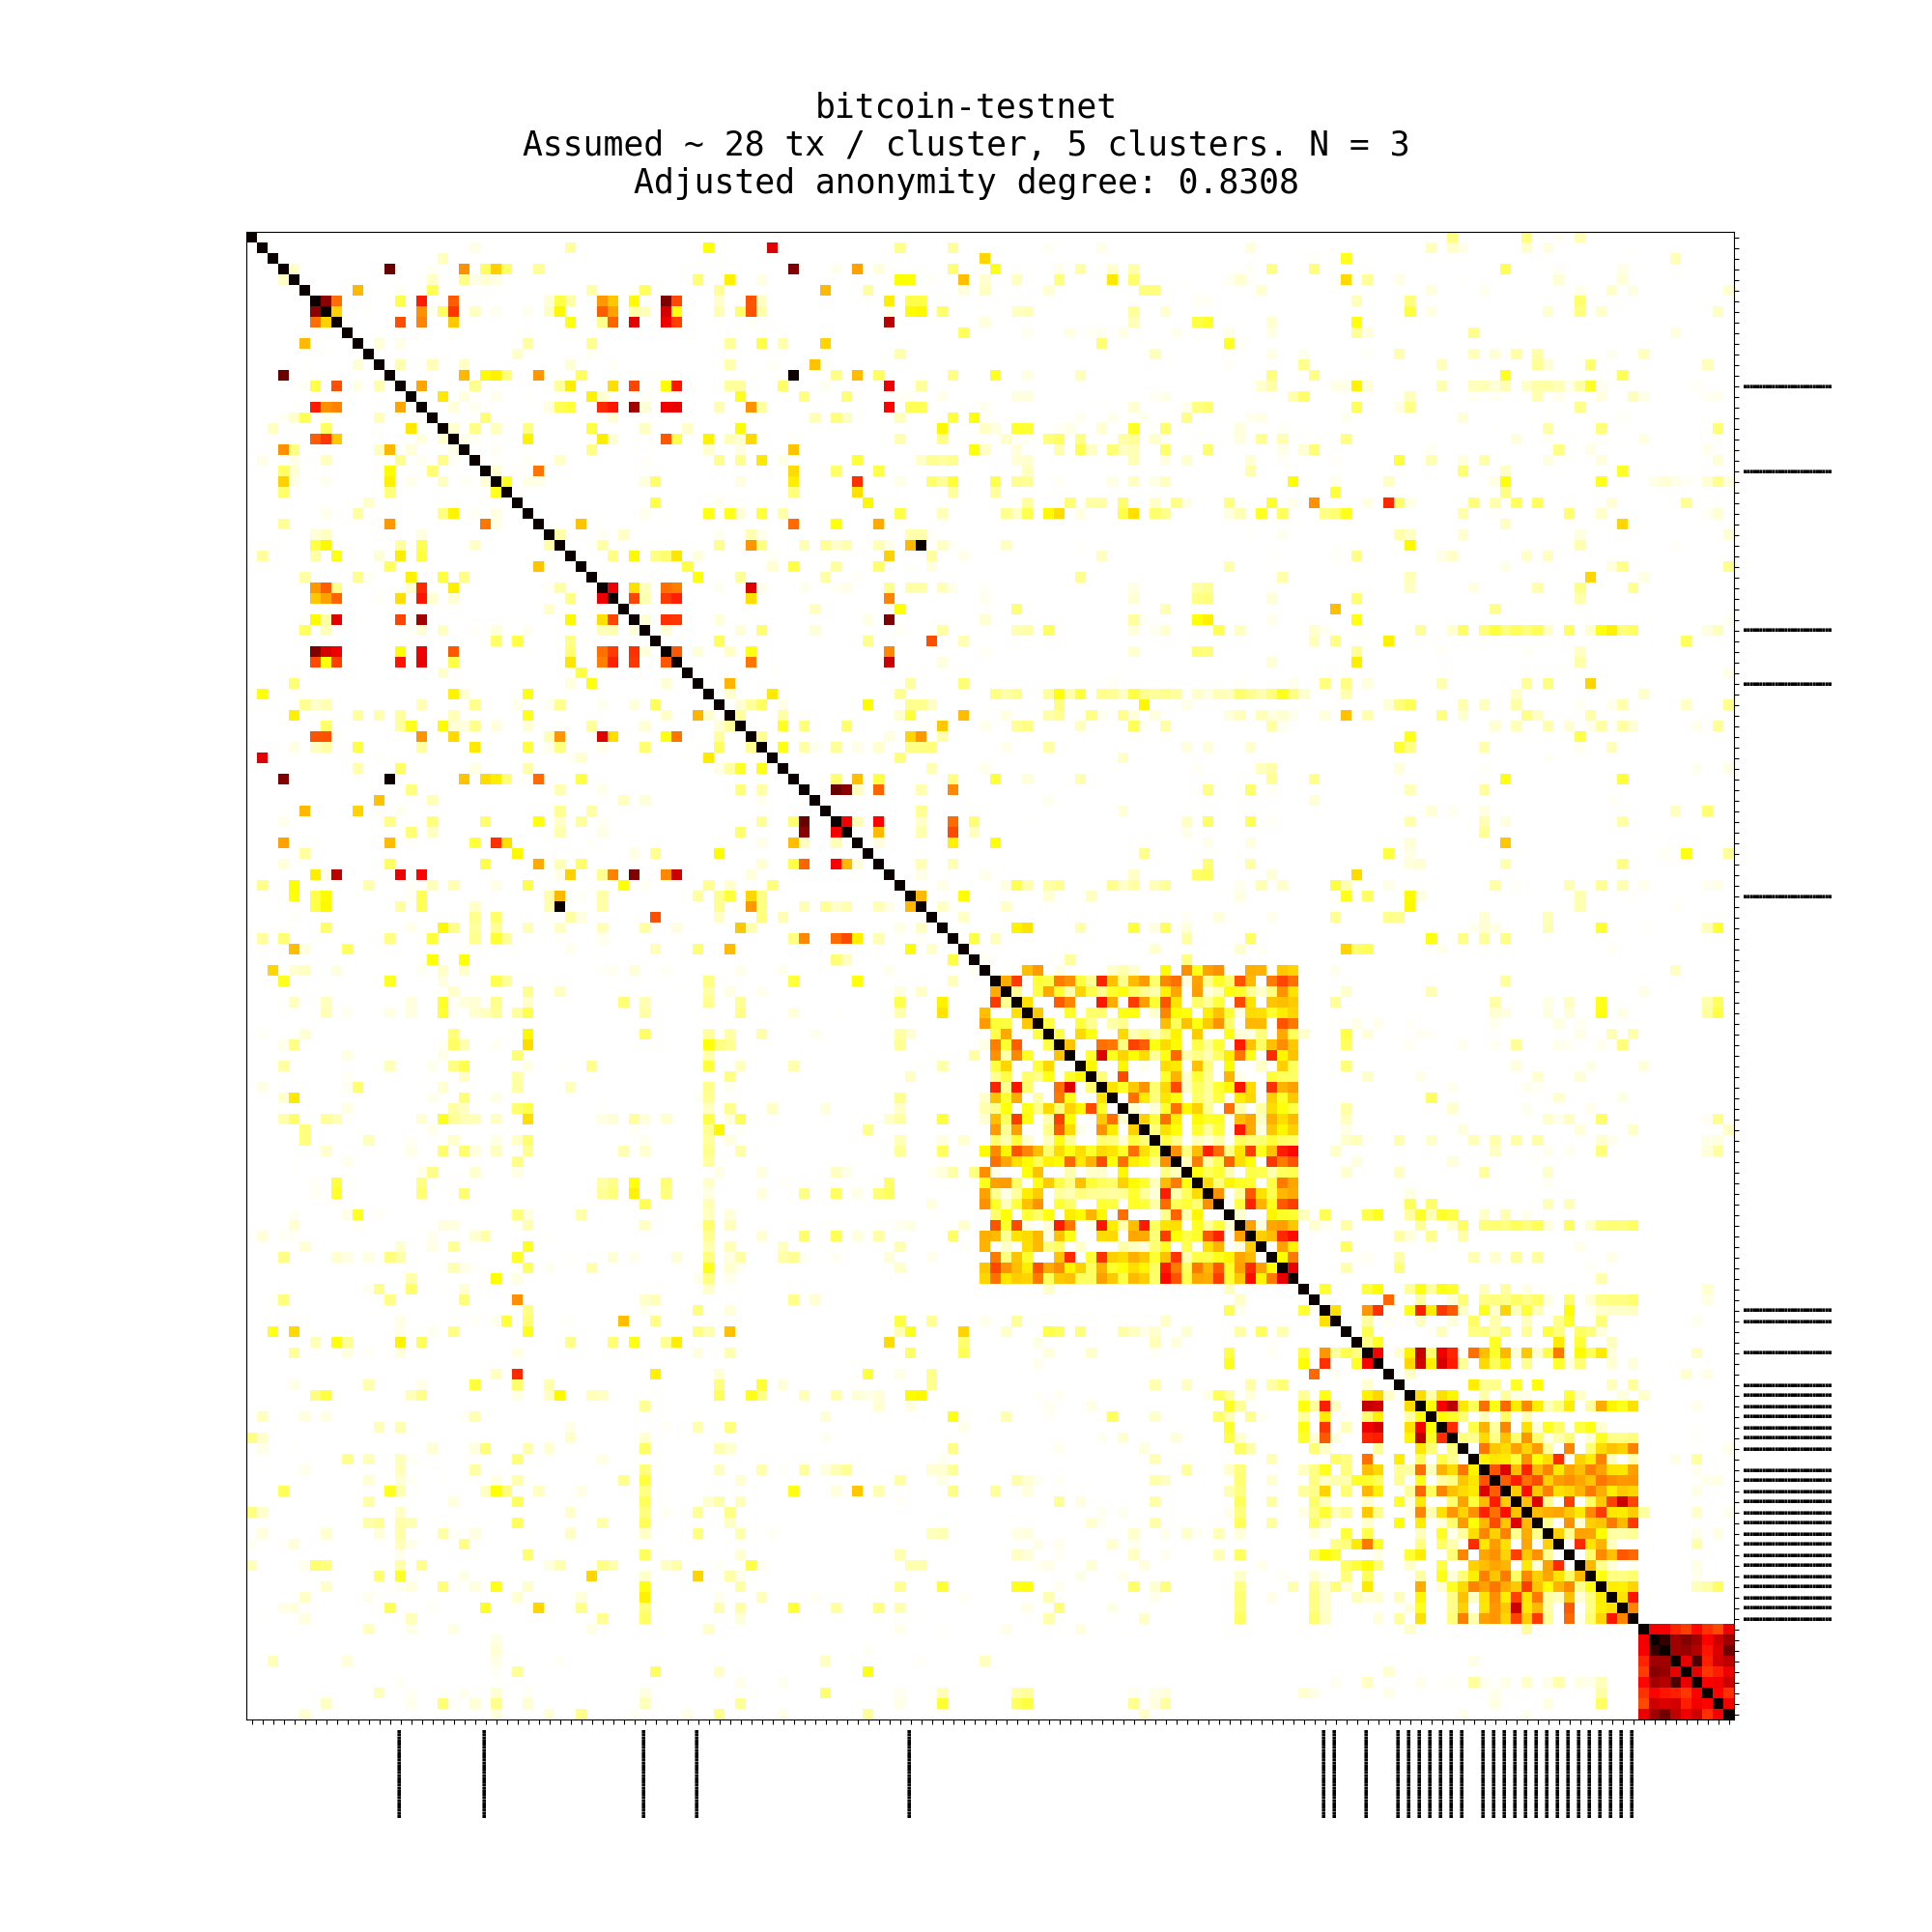
\includegraphics[width=\columnwidth]{bitcoin-testnet-1541509693-California.png}
		\caption{Bitcoin testnet (California)}
	\end{minipage}\hfill
	\begin{minipage}{0.5\textwidth}
		\centering
		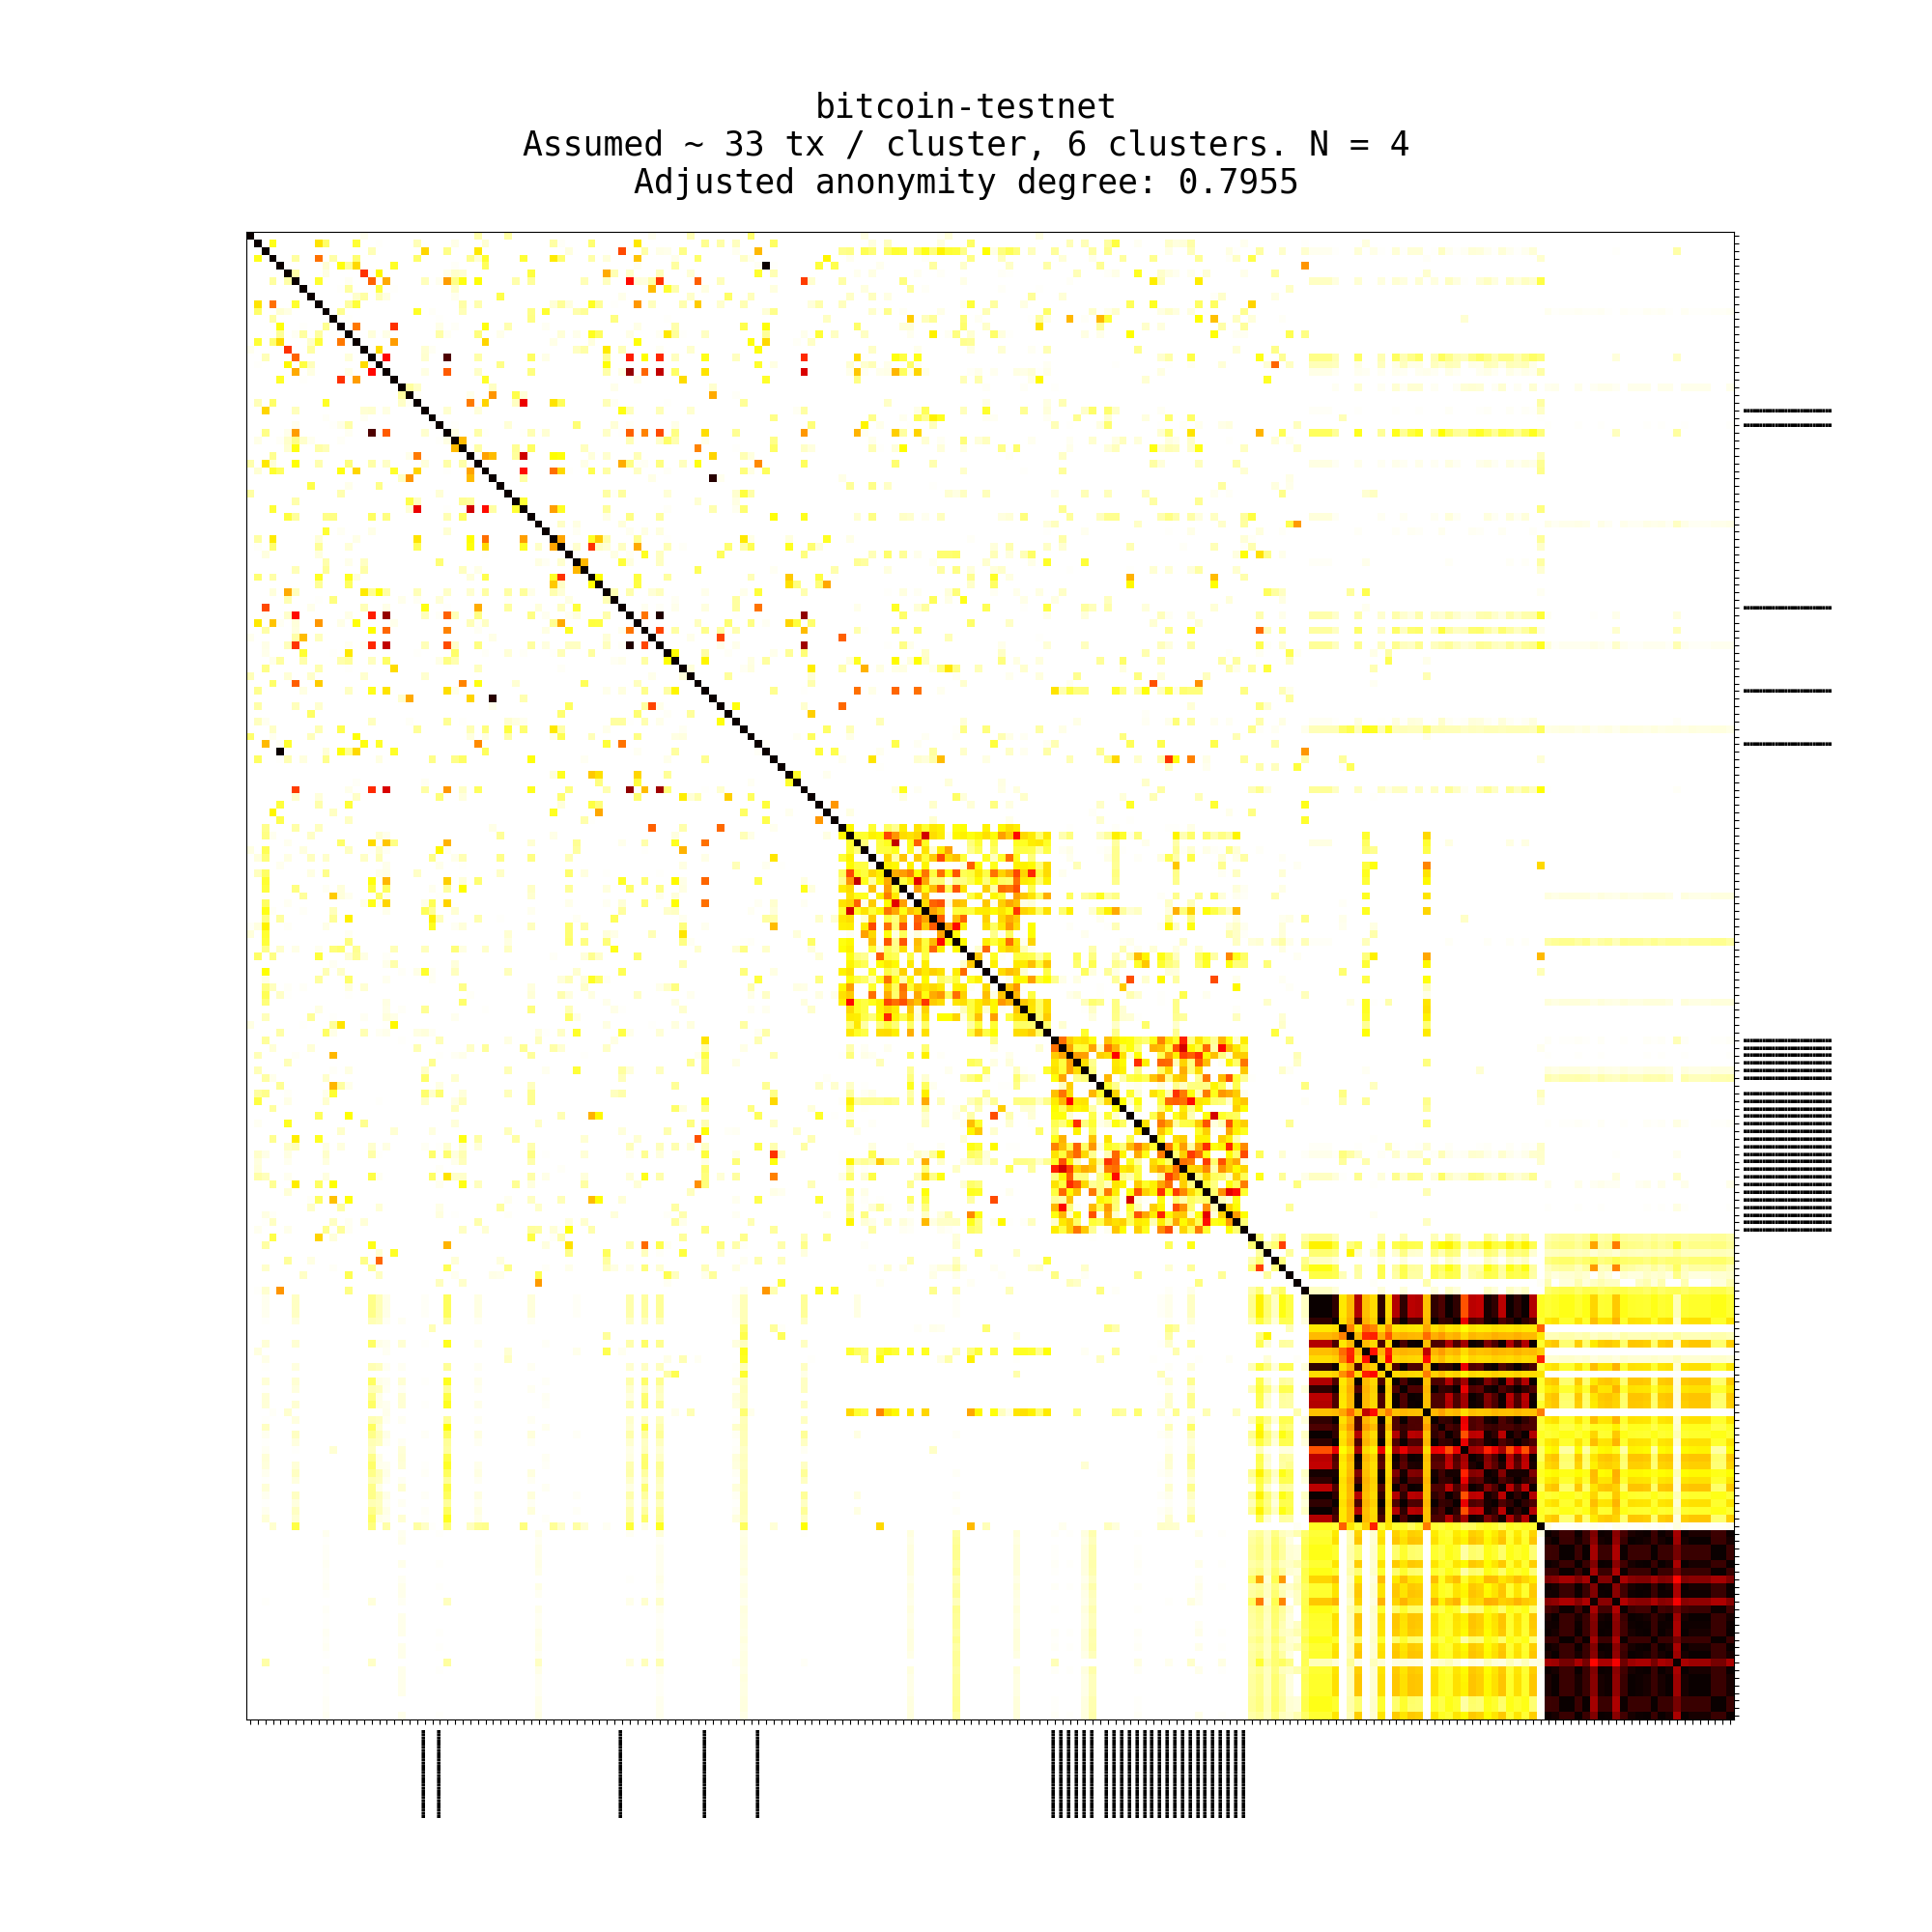
\includegraphics[width=\columnwidth]{bitcoin-testnet-1541511845-Tokyo.png}
		\caption{Bitcoin testnet (Tokyo)}
	\end{minipage}\hfill
	\label{fig:bitcoin-testnet-1}
\end{figure*}

\begin{figure*}
	\centering
	\begin{minipage}{0.5\textwidth}
		\centering
		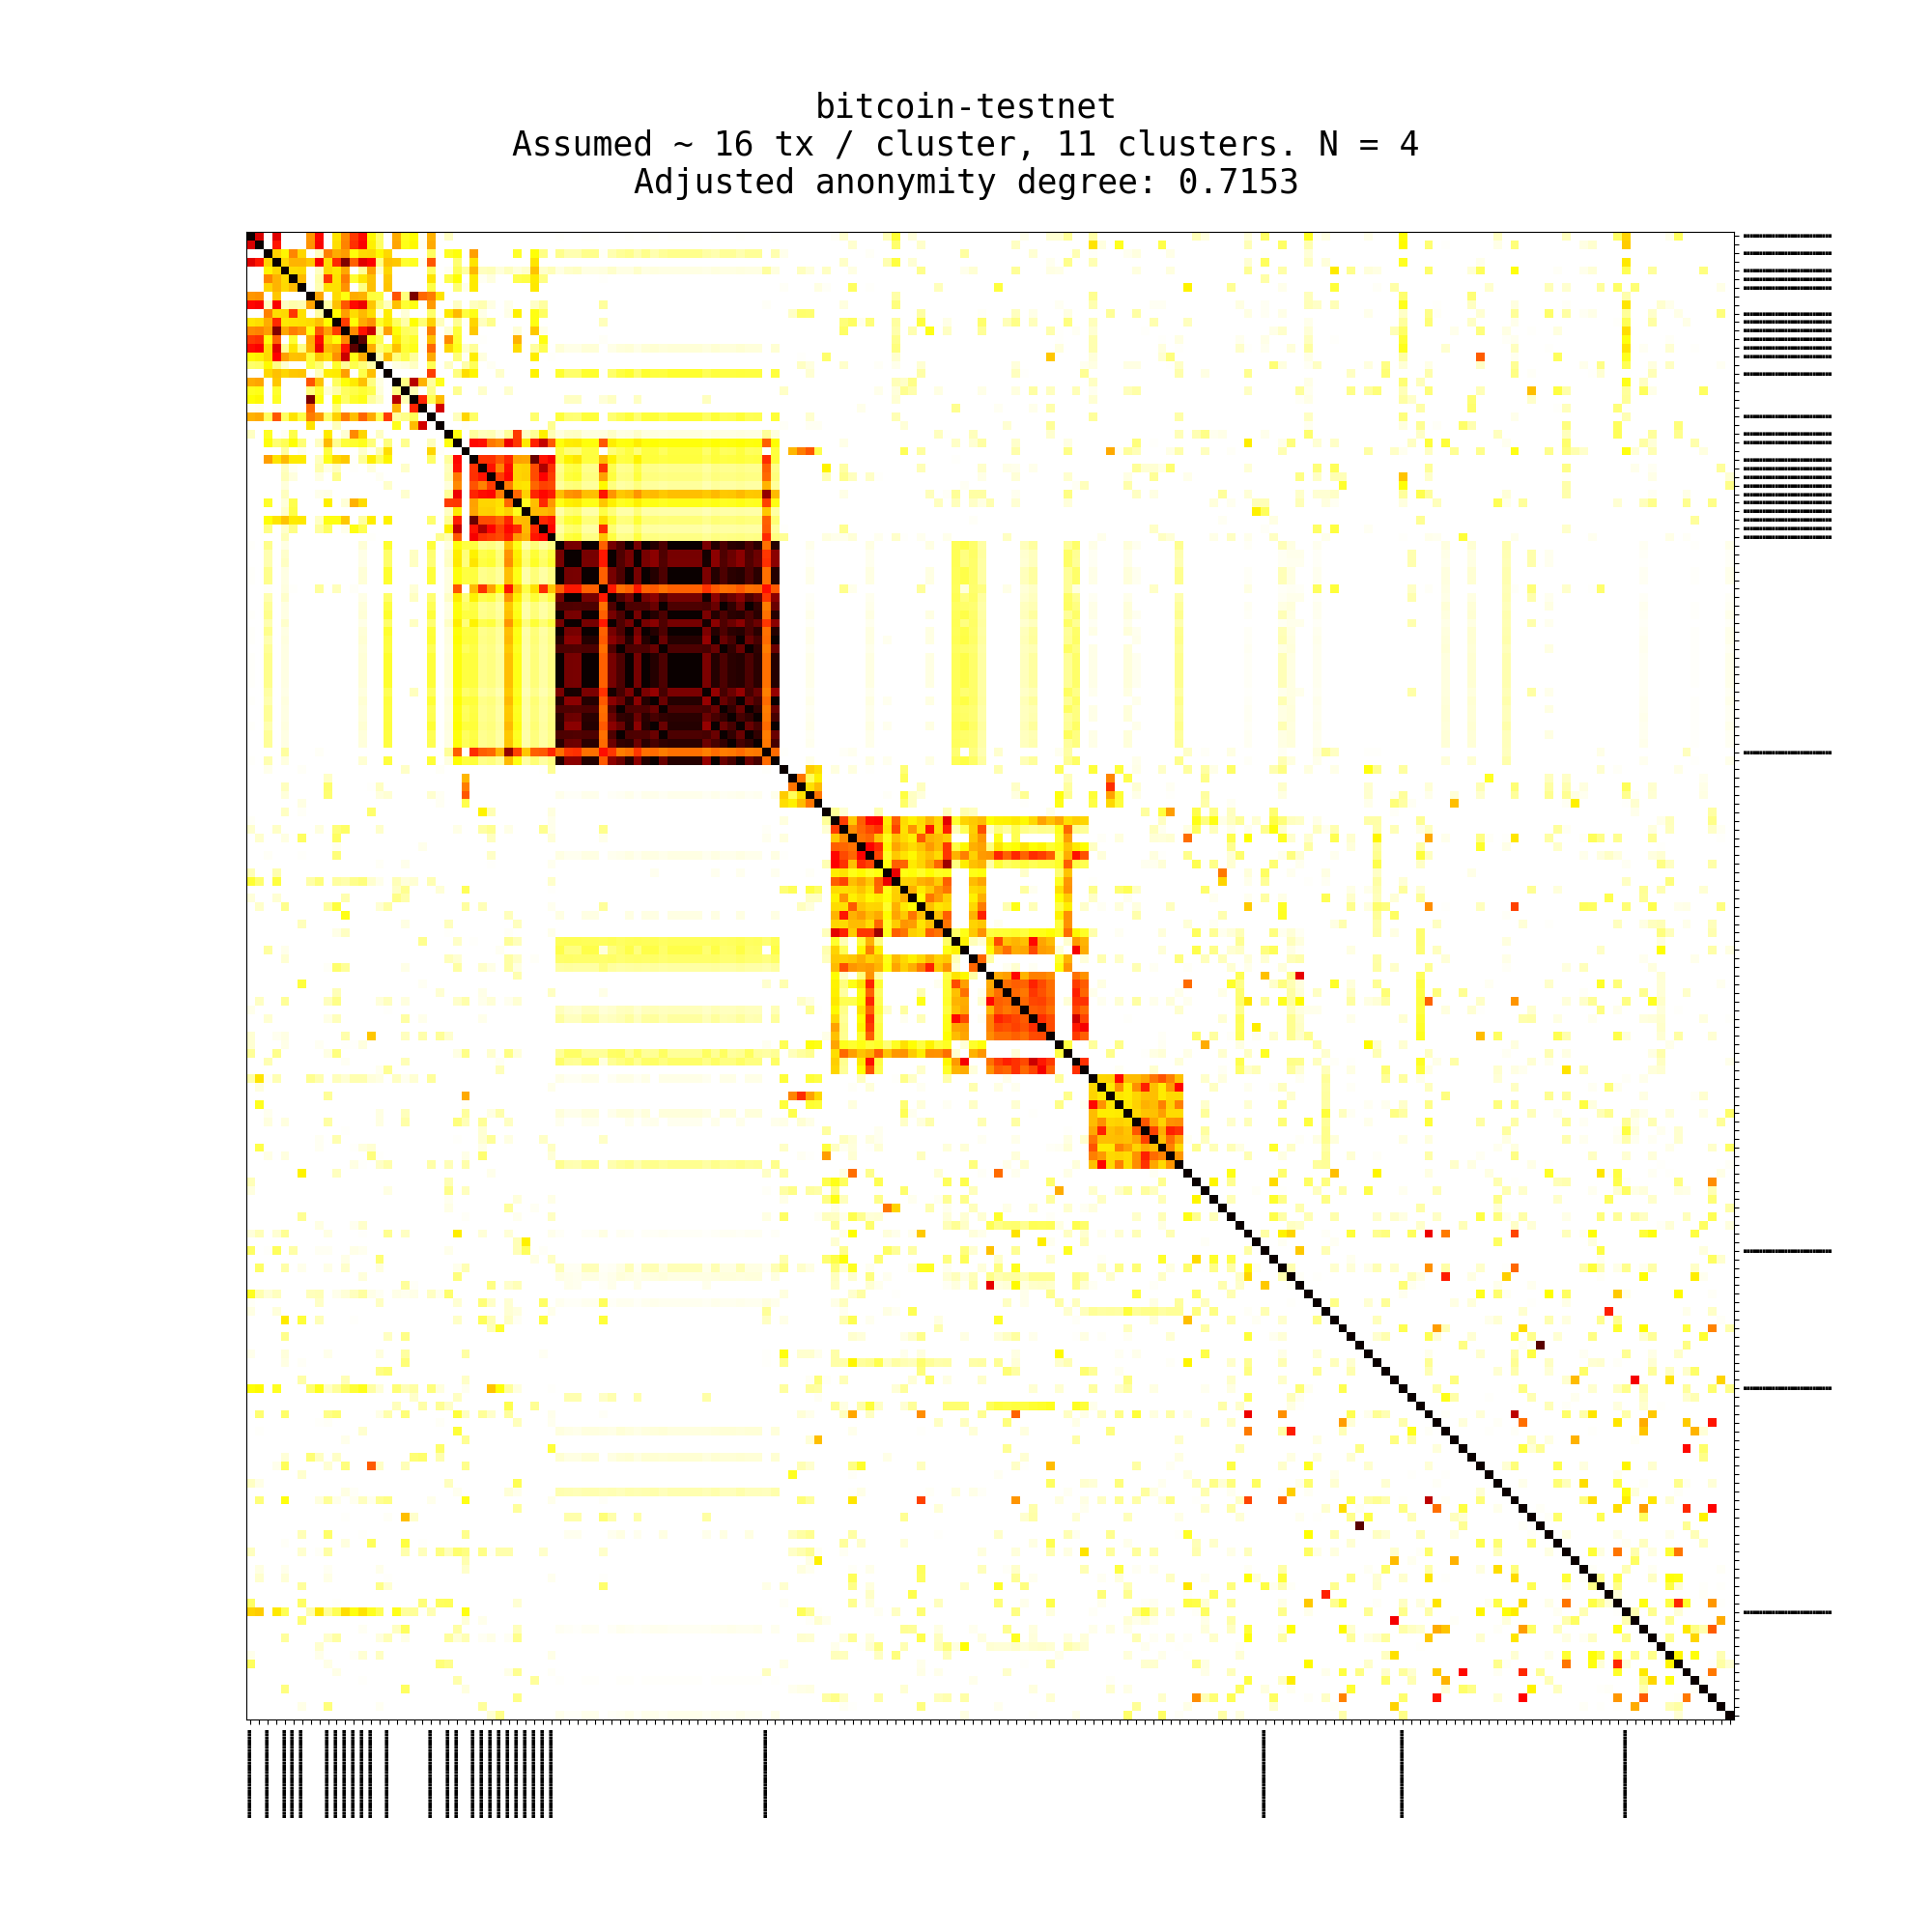
\includegraphics[width=\columnwidth]{bitcoin-testnet-1541513977-Frankfurt.png}
		\caption{Bitcoin testnet (Frankfurt)}
	\end{minipage}\hfill
	\begin{minipage}{0.5\textwidth}
		\centering
		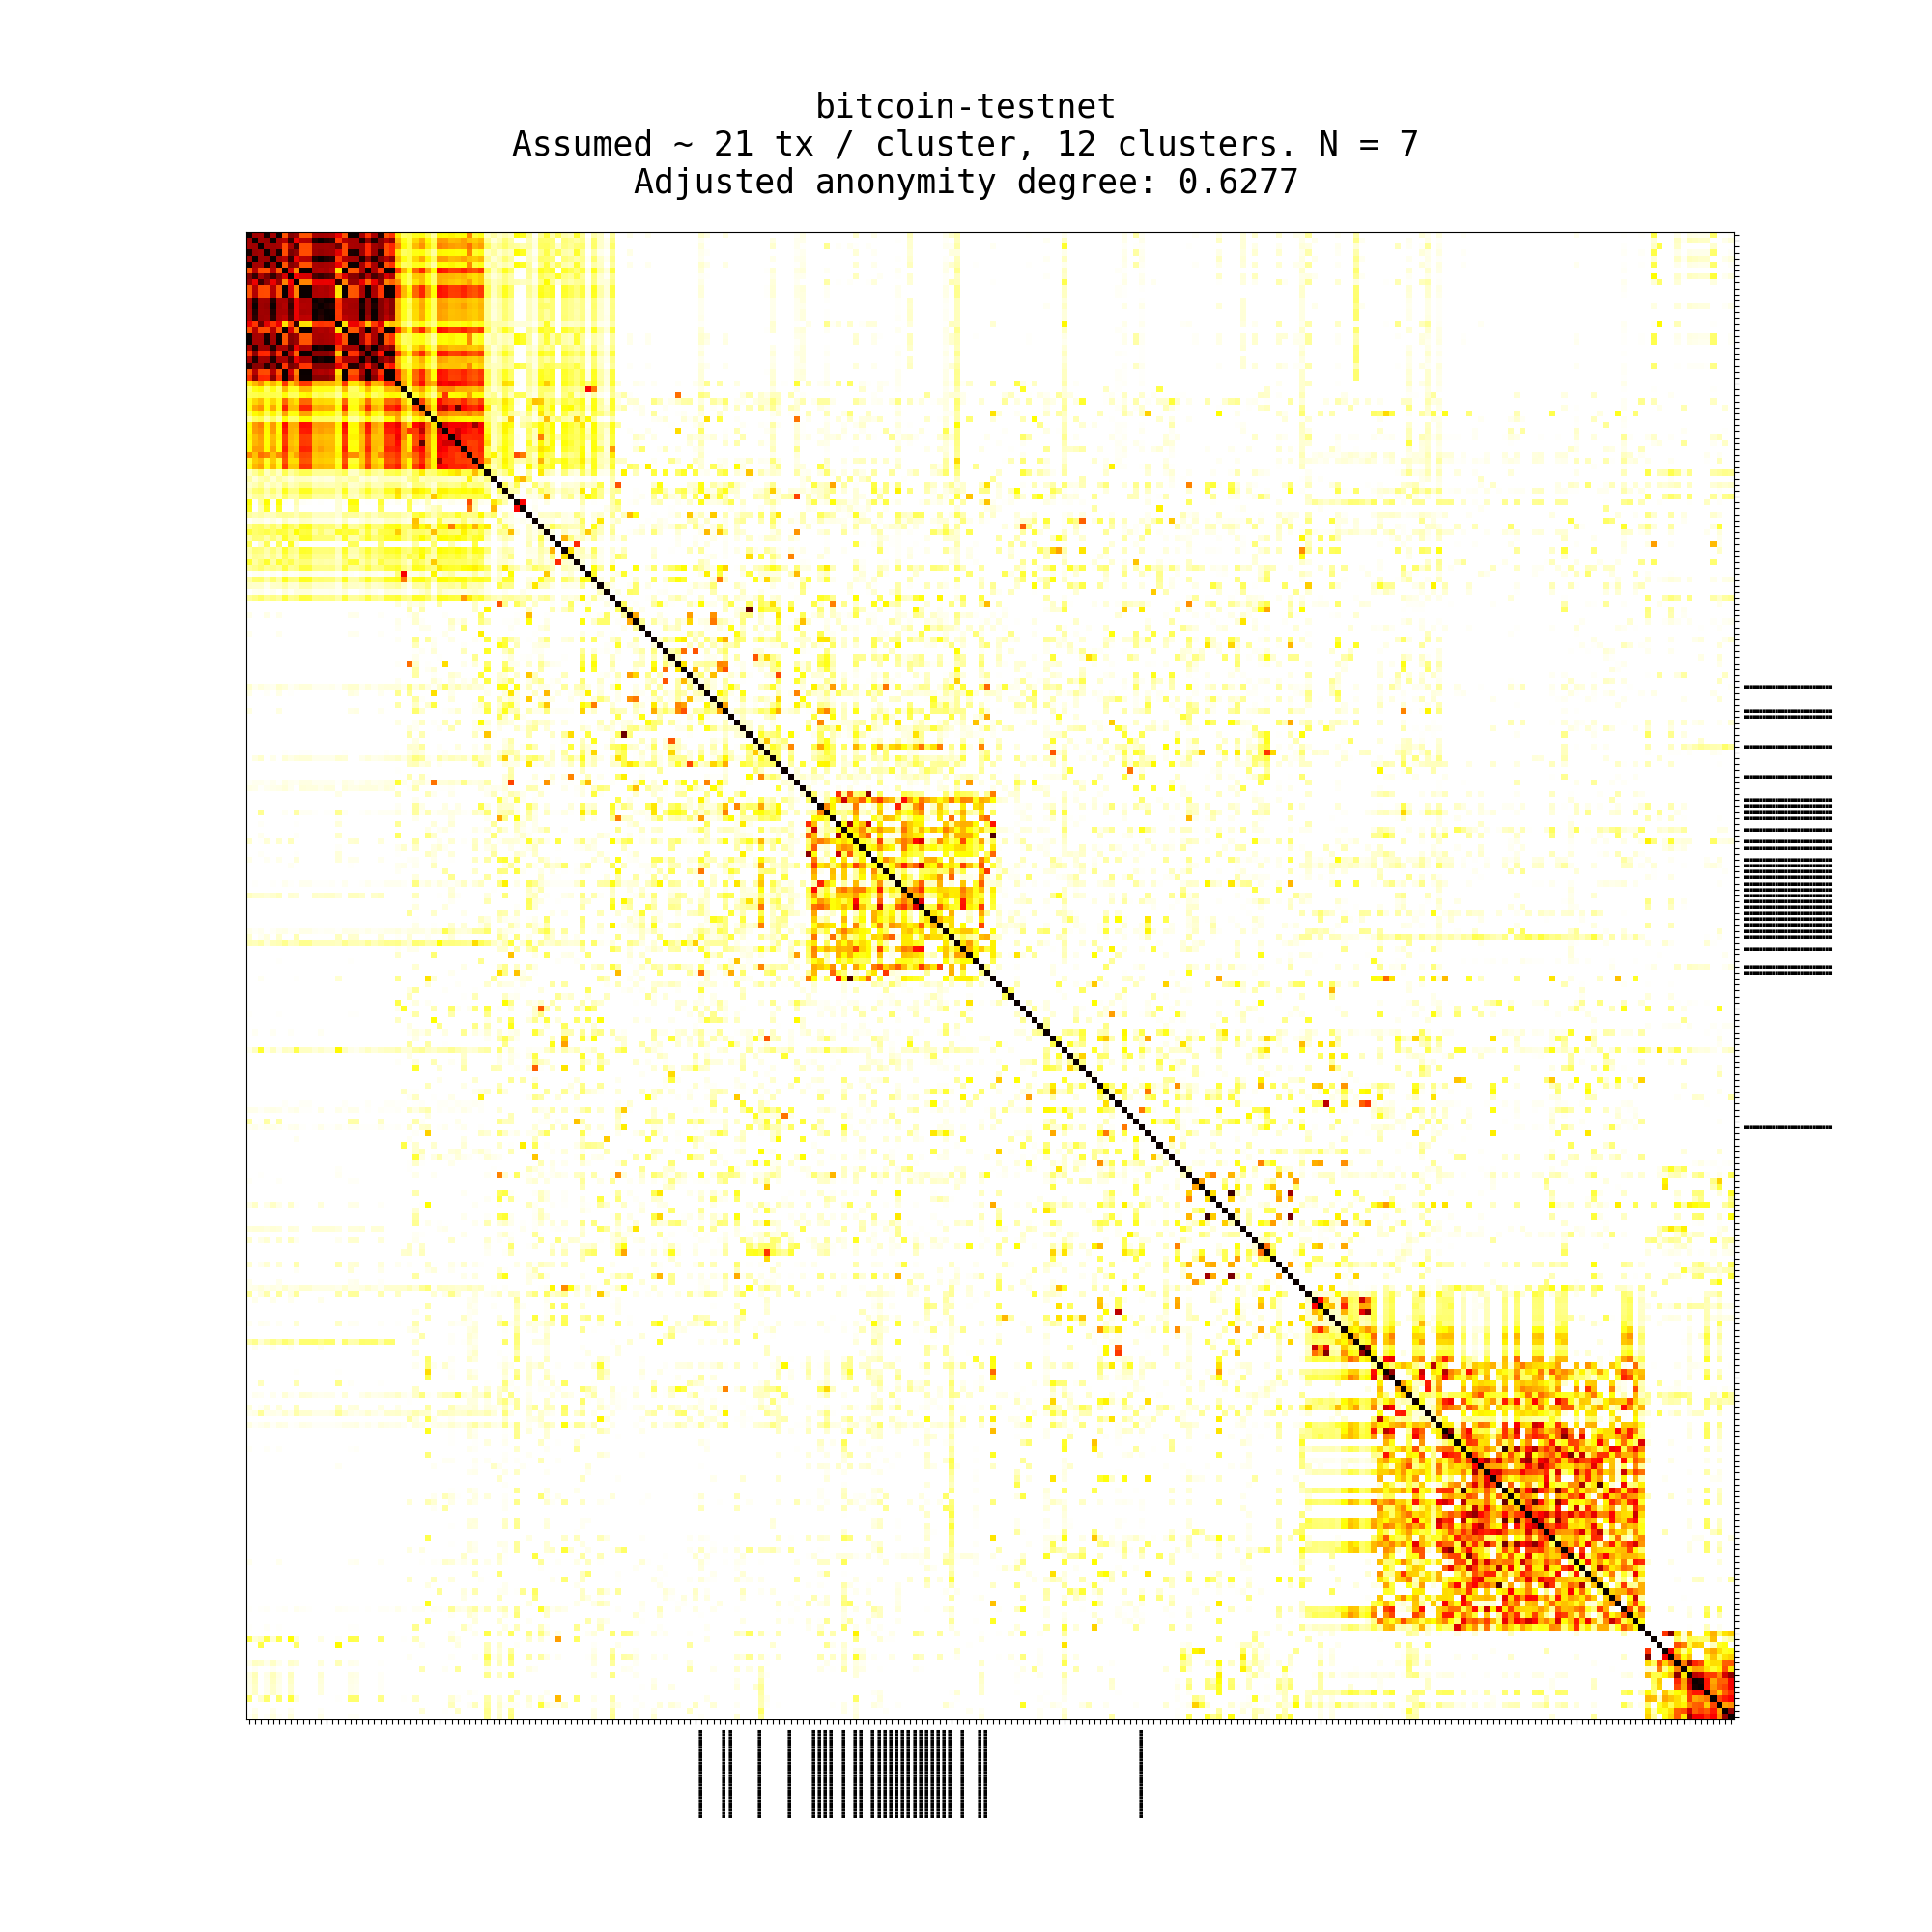
\includegraphics[width=\columnwidth]{bitcoin-testnet-1541516997-combined.png}
		\caption{Bitcoin testnet (combined)}
	\end{minipage}\hfill
	\label{fig:bitcoin-testnet-2}
\end{figure*}


\paragraph{Estimating the original IP}

We use the ADDR messages to determine (with some level of precision) the IP of the node which issued the transactions in the control group.
In our experiments, we first launch the listener, and only then launch the issuing nodes.
This means that the listener captures the ADDR messages issued by the issuing nodes during bootstrapping.
Address messages propagate through the network more slowly than transactions, which are relayed to all nodes' neighbors with relatively small random delays.
A node listening to network traffic can therefore distinguish between messages containing addresses of recently joined nodes and re-broadcasts of older addresses messages.
If an IP is relayed from 1 or 2 nodes, which is most often the case, we assume these IP addresses are old re-broadcasts.
If an IP is relayed from a higher number of nodes, we assume the node at the relayed IP either has just joined the network or is re-advertising its IP after an approximately 24~hours delay.

Our idea is to leverage the \texttt{ADDR} messages as follows.
For each cluster, we determine the IPs of the most "important" nodes, i.e.,~nodes we assume are entry nodes of the transaction originator.
For each transaction in the cluster, we sum up the weights of all IPs which relayed it to us.
The top 10\% of most weighted IPs are assumed to be the entry nodes.
Looking at propagation of \texttt{ADDR} messages, the intuition is that an \texttt{ADDR} message relayed by a set of IPs which substantially intersects with assumed entry nodes of cluster X is the IP address of the node which issued the transactions.
We define an IP to "likely" correspond to the transactions originator if it was relayed to us in an \texttt{ADDR} message by a set of IPs which overlap with assumed entry nodes determined on the previous step.
Applying this technique to the Bitcoin testnet experiments, in 3 experiments out of 4 the right IP appeared in the top 5 most likely originator IPs for clusters which consist mostly of control transactions.
This result indicates that in addition to being able to estimate with high accuracy whether given two transactions were issued by the same node, an adversary can narrow down the search for the IP of the transaction source to a handful of IPs.
This may give the attacker valuable information, including the approximate geographical location of the victim.

\subsubsection{Bitcoin mainnet}

For Bitcoin mainnet, we performed one experiment with a listener located in Frankfurt.
An experiment on Bitcoin mainnet showed that transactions also exhibit the "clustering" behavior, though the results are weaker because of a much larger transaction rate and due to the fact that we only connected to 1000~servers (asking for up to 50~connections).
We used learning and control transaction sets of 20~transactions each; 5 transactions from the control set were assumed "known" for anonymity degree calculation.

\begin{figure}[!t]
	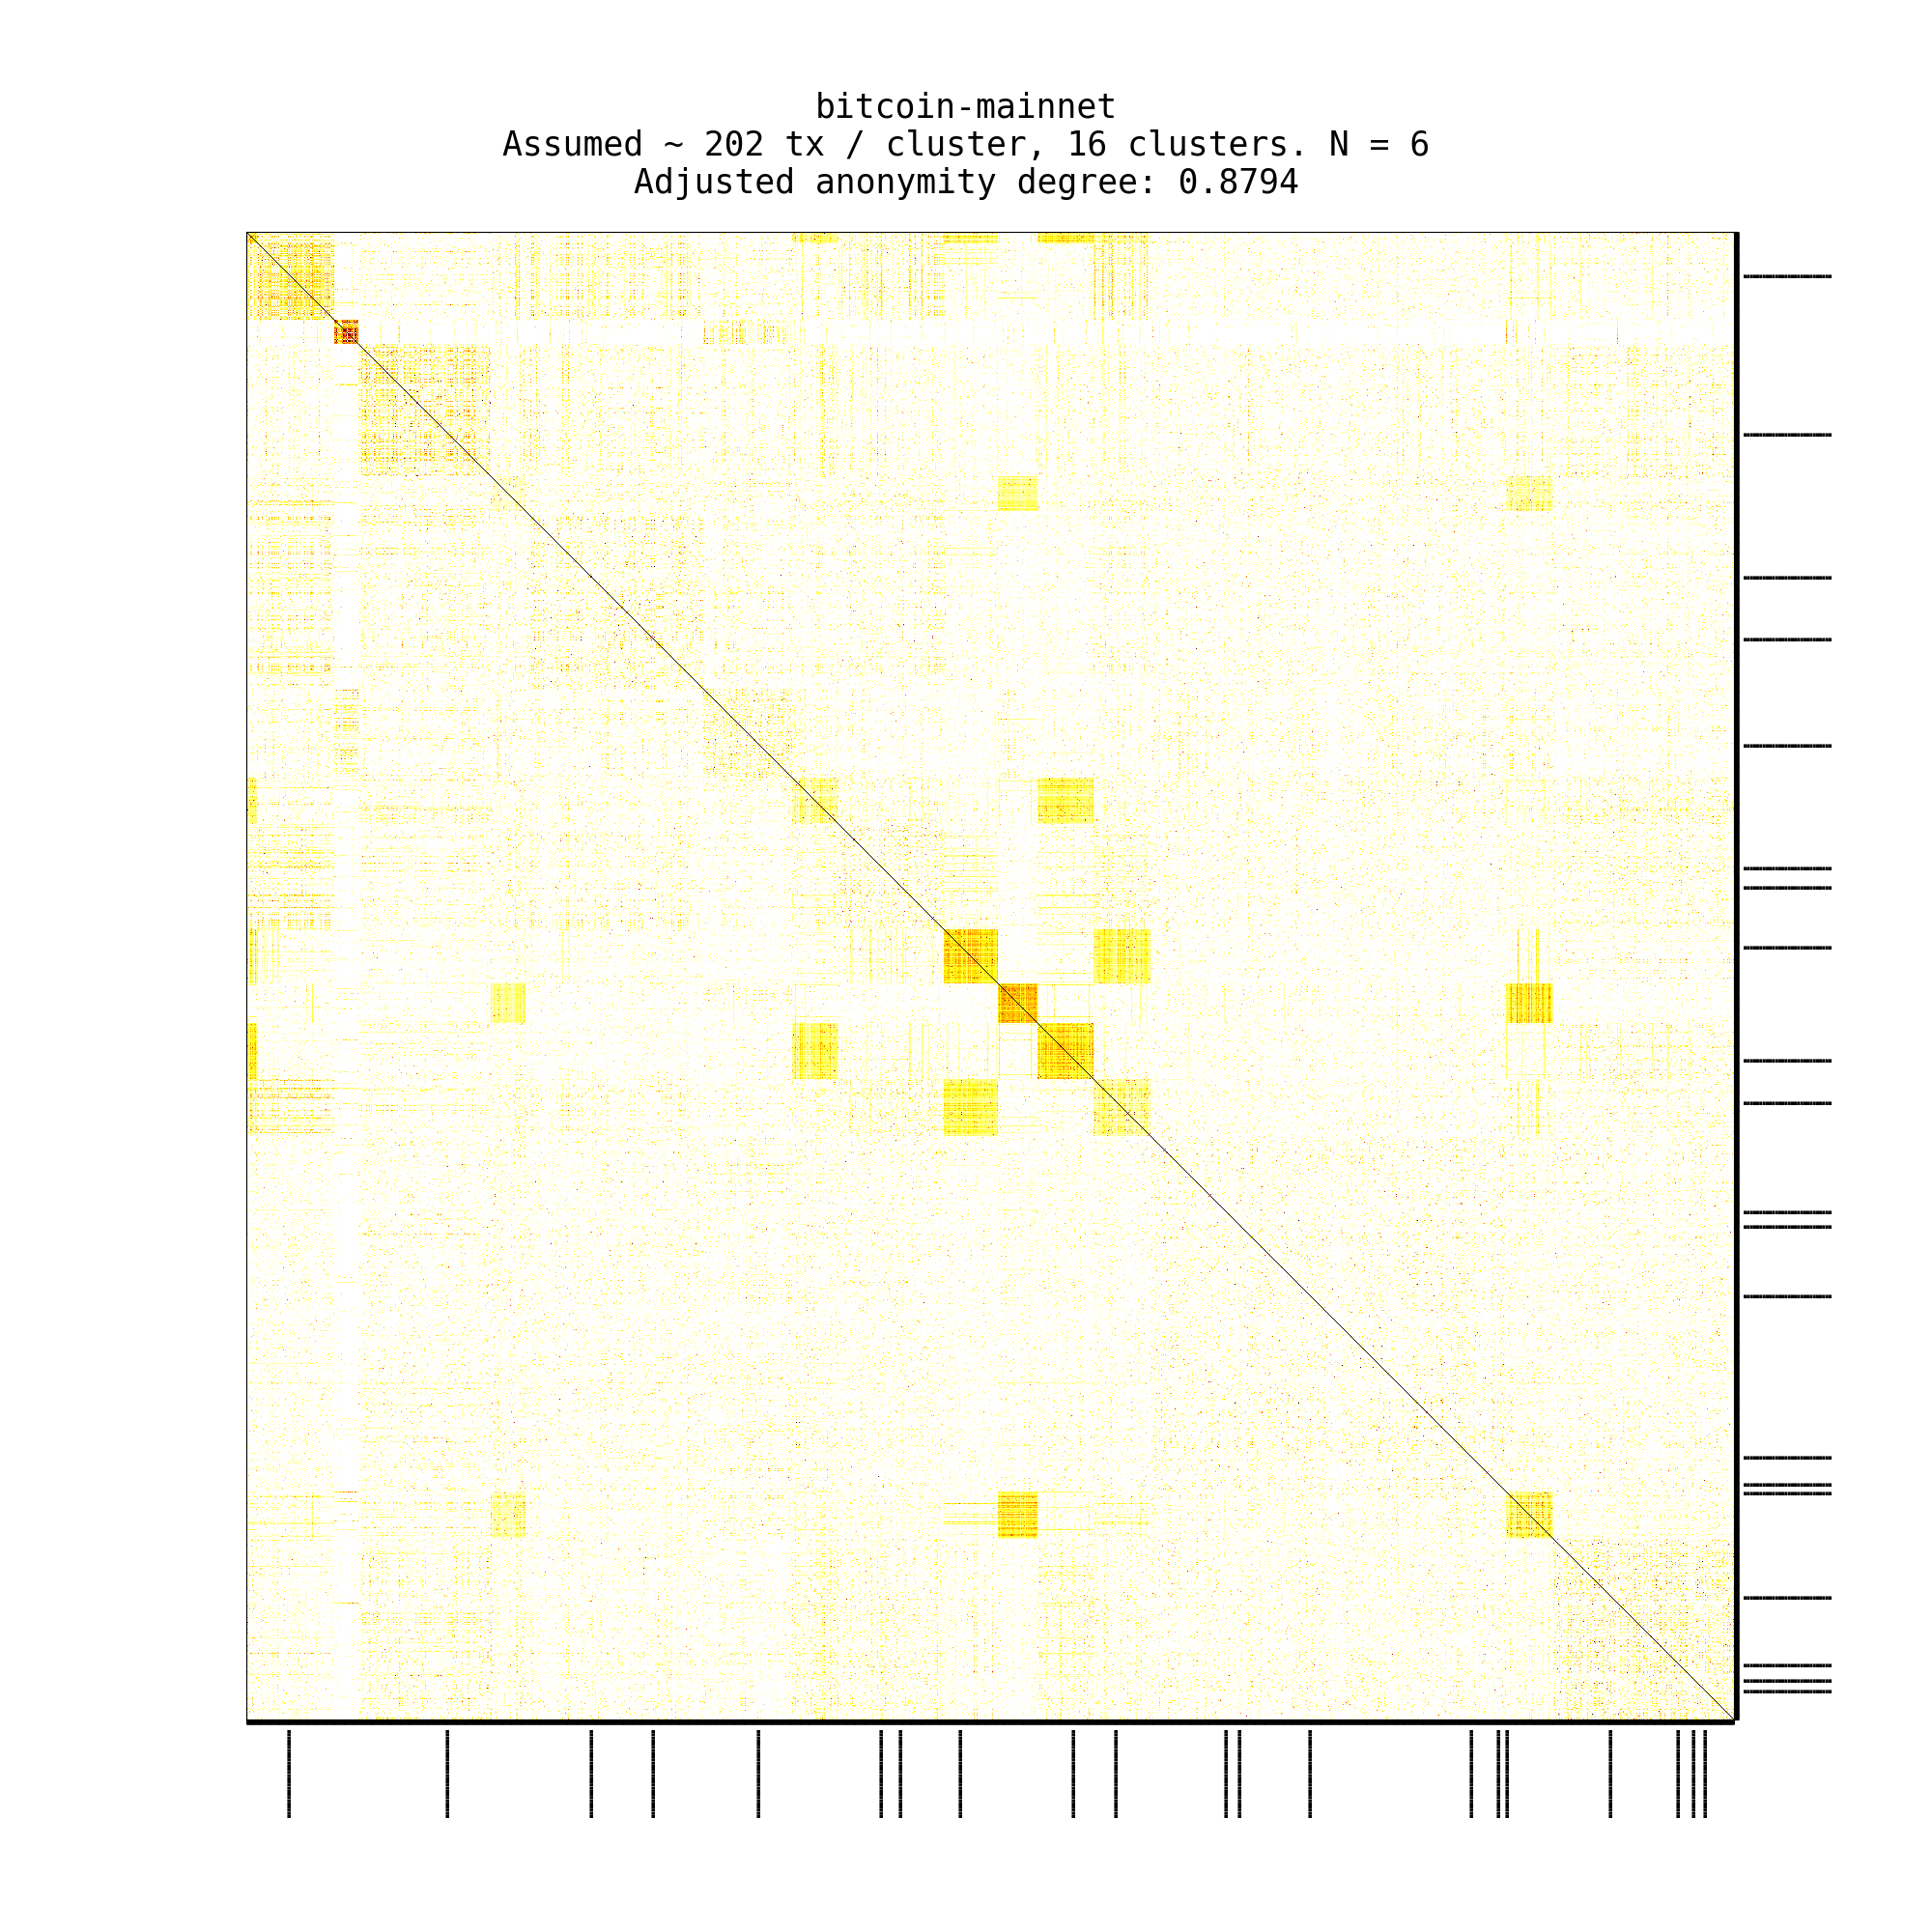
\includegraphics[width=\columnwidth]{bitcoin-mainnet-1542054034-fig-correlations-202-txcl-006-N-Rand-best.png}
	\caption{Bitcoin mainnet}
	\label{fig:bitoin-mainnet}
\end{figure}


\subsubsection{Zcash}

For the Zcash mainnet, we performed one experiment with a listener located in Frankfurt.
The learning and control sets consist of 20 and 18~transactions respectively; 8~out of 18 control transactions are shielded (from a t-address to a z-address).
We use 6~control transactions as "known" for anonymity degree estimation.
The Zcash network is much smaller than the Bitcoin testnet.
Moreover, Zcash servers have far fewer free slots on average (36 against 64 on Bitcoin testnet).
We notice that relatively many servers only provide our listener with 1 -- 10 slots.
This may indicate a larger share of "protected" nodes, i.e.,~nodes which are configured (using firewalls or other network-level means) to only provide a limited number of connections to each IP.
Note than a resourceful adversary may overcome this limitation by purchasing additional IP addresses from a cloud provider.

Zcash does not provide privacy by default: zk-SNARKs are used only in transactions involving \textit{shielded} addresses~\cite{Kappos2018}.
The majority of transactions happen between \textit{transparent} addresses and have no additional privacy-preserving mechanisms compared to Bitcoin.

\begin{figure}[!t]
	\centering
	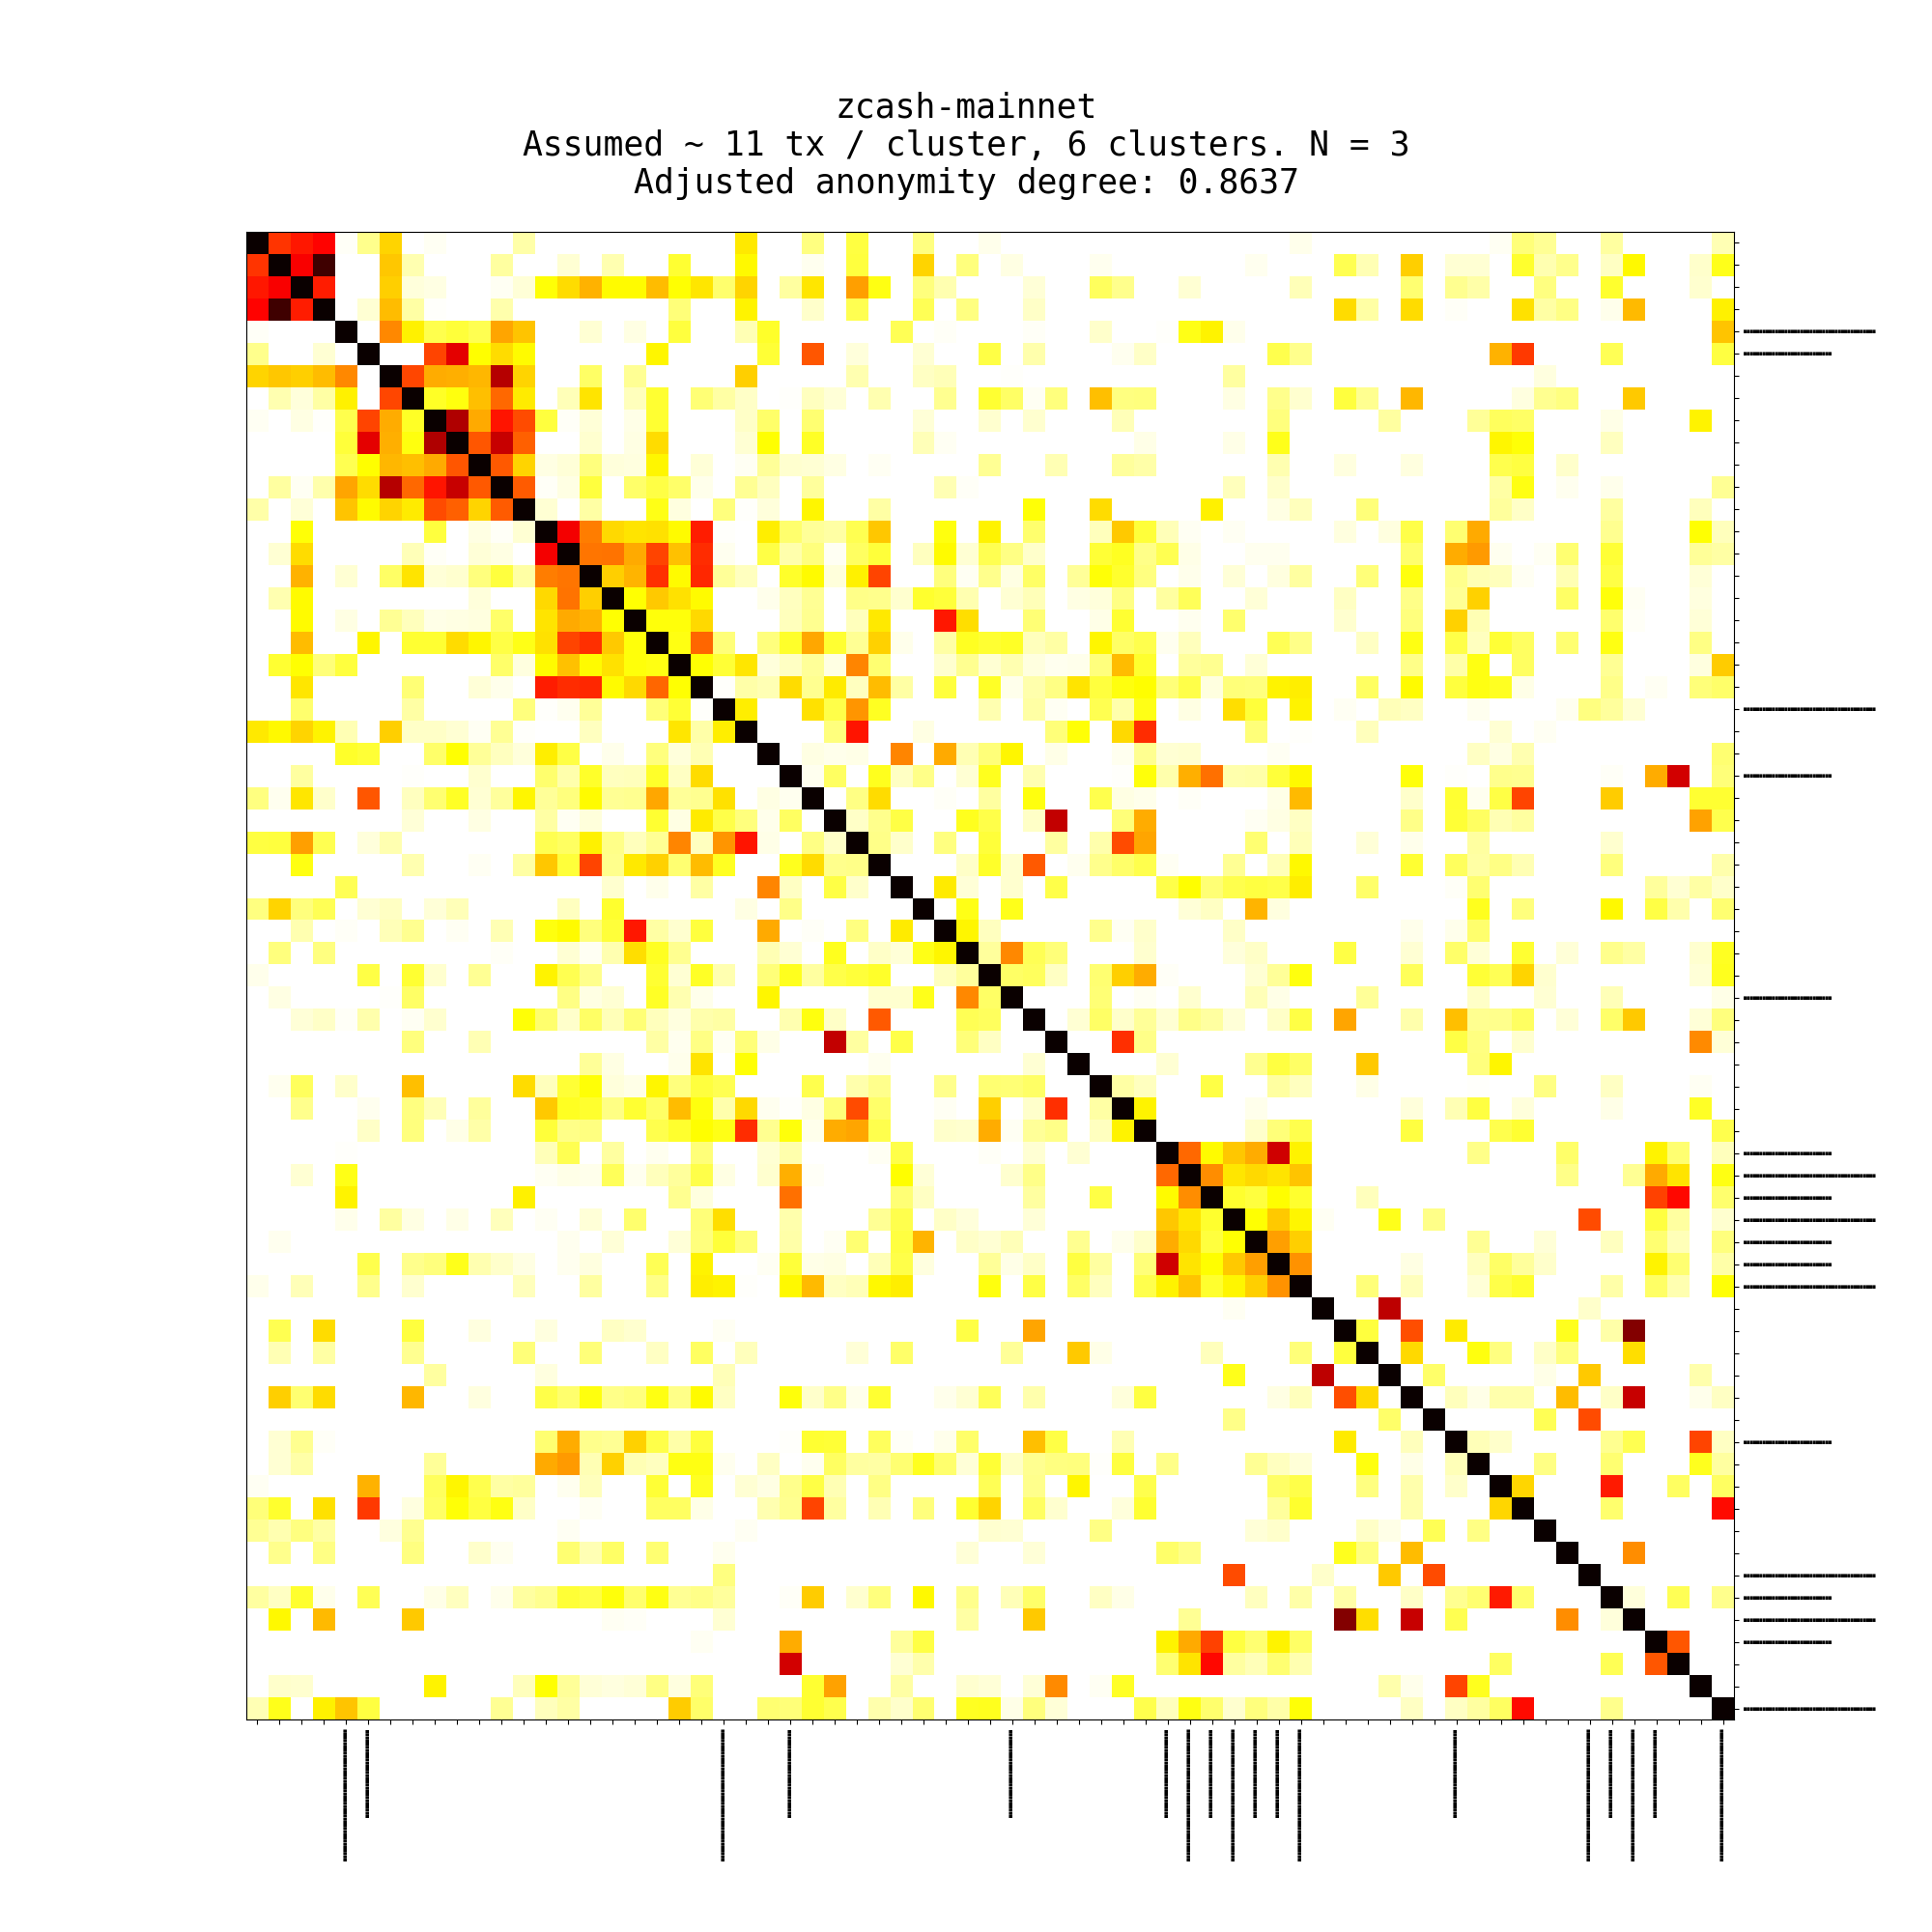
\includegraphics[width=\columnwidth]{zcash-mainnet-1541938472-Frankfurt.png}
	\caption{Zcash}
	\label{fig:zcash-mainnet}
\end{figure}

\begin{figure*}
	\centering
	\begin{minipage}{0.5\textwidth}
		\centering
		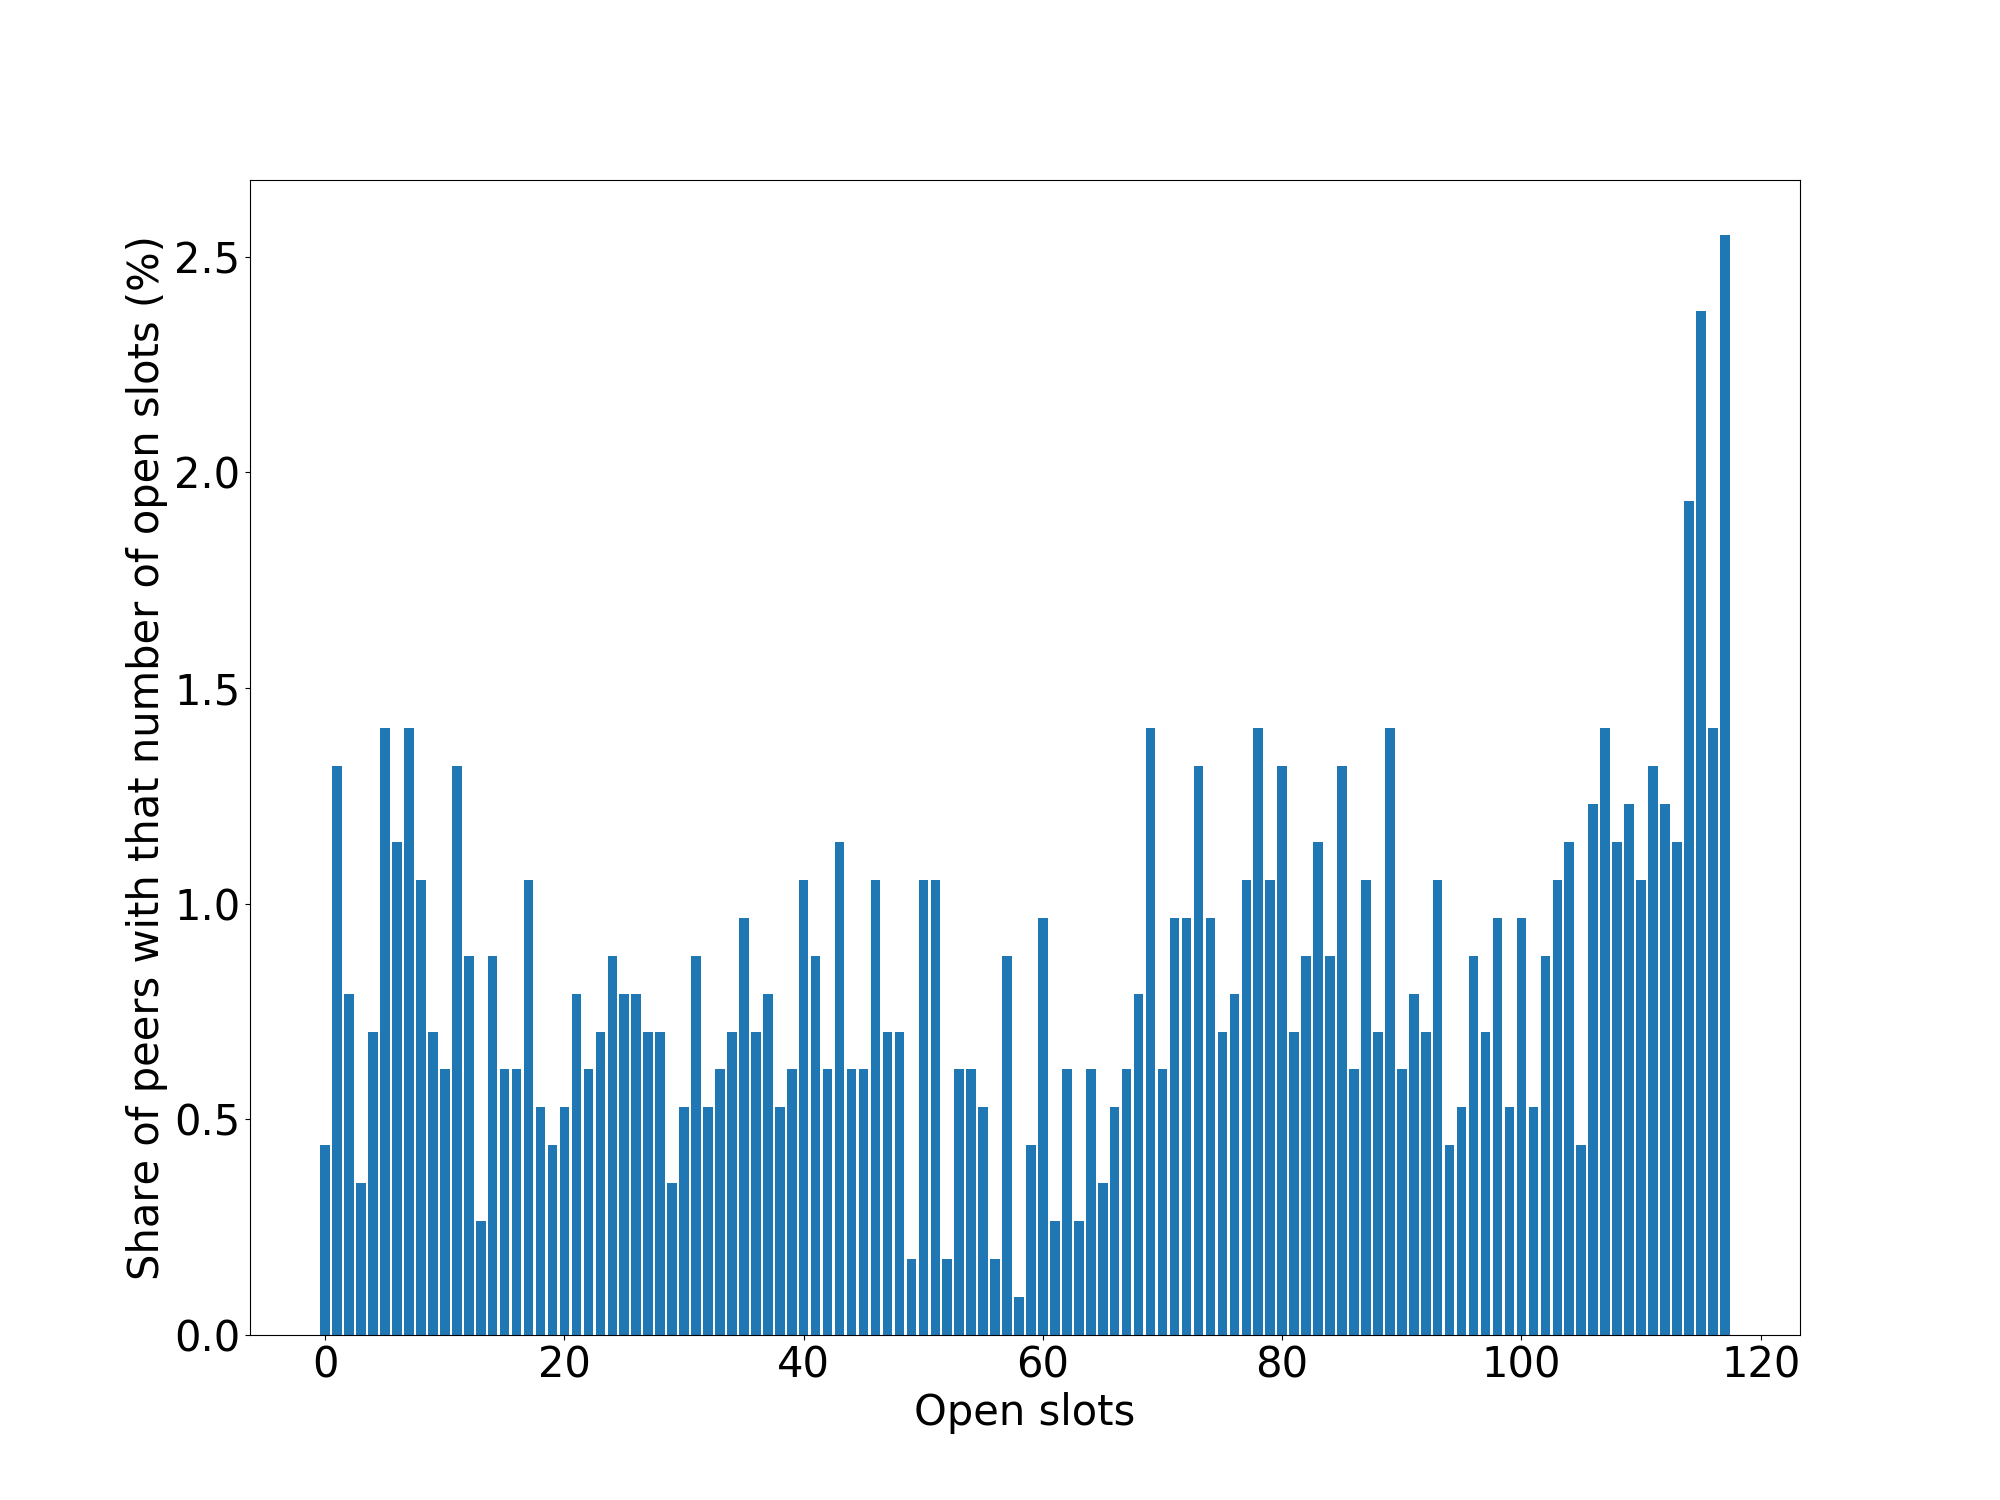
\includegraphics[width=\columnwidth]{bitcoin-testnet-1541513977-conn-max-histogram.png}
		\caption{Free slots: Bitcoin testnet}
	\end{minipage}\hfill
	\begin{minipage}{0.5\textwidth}
		\centering
		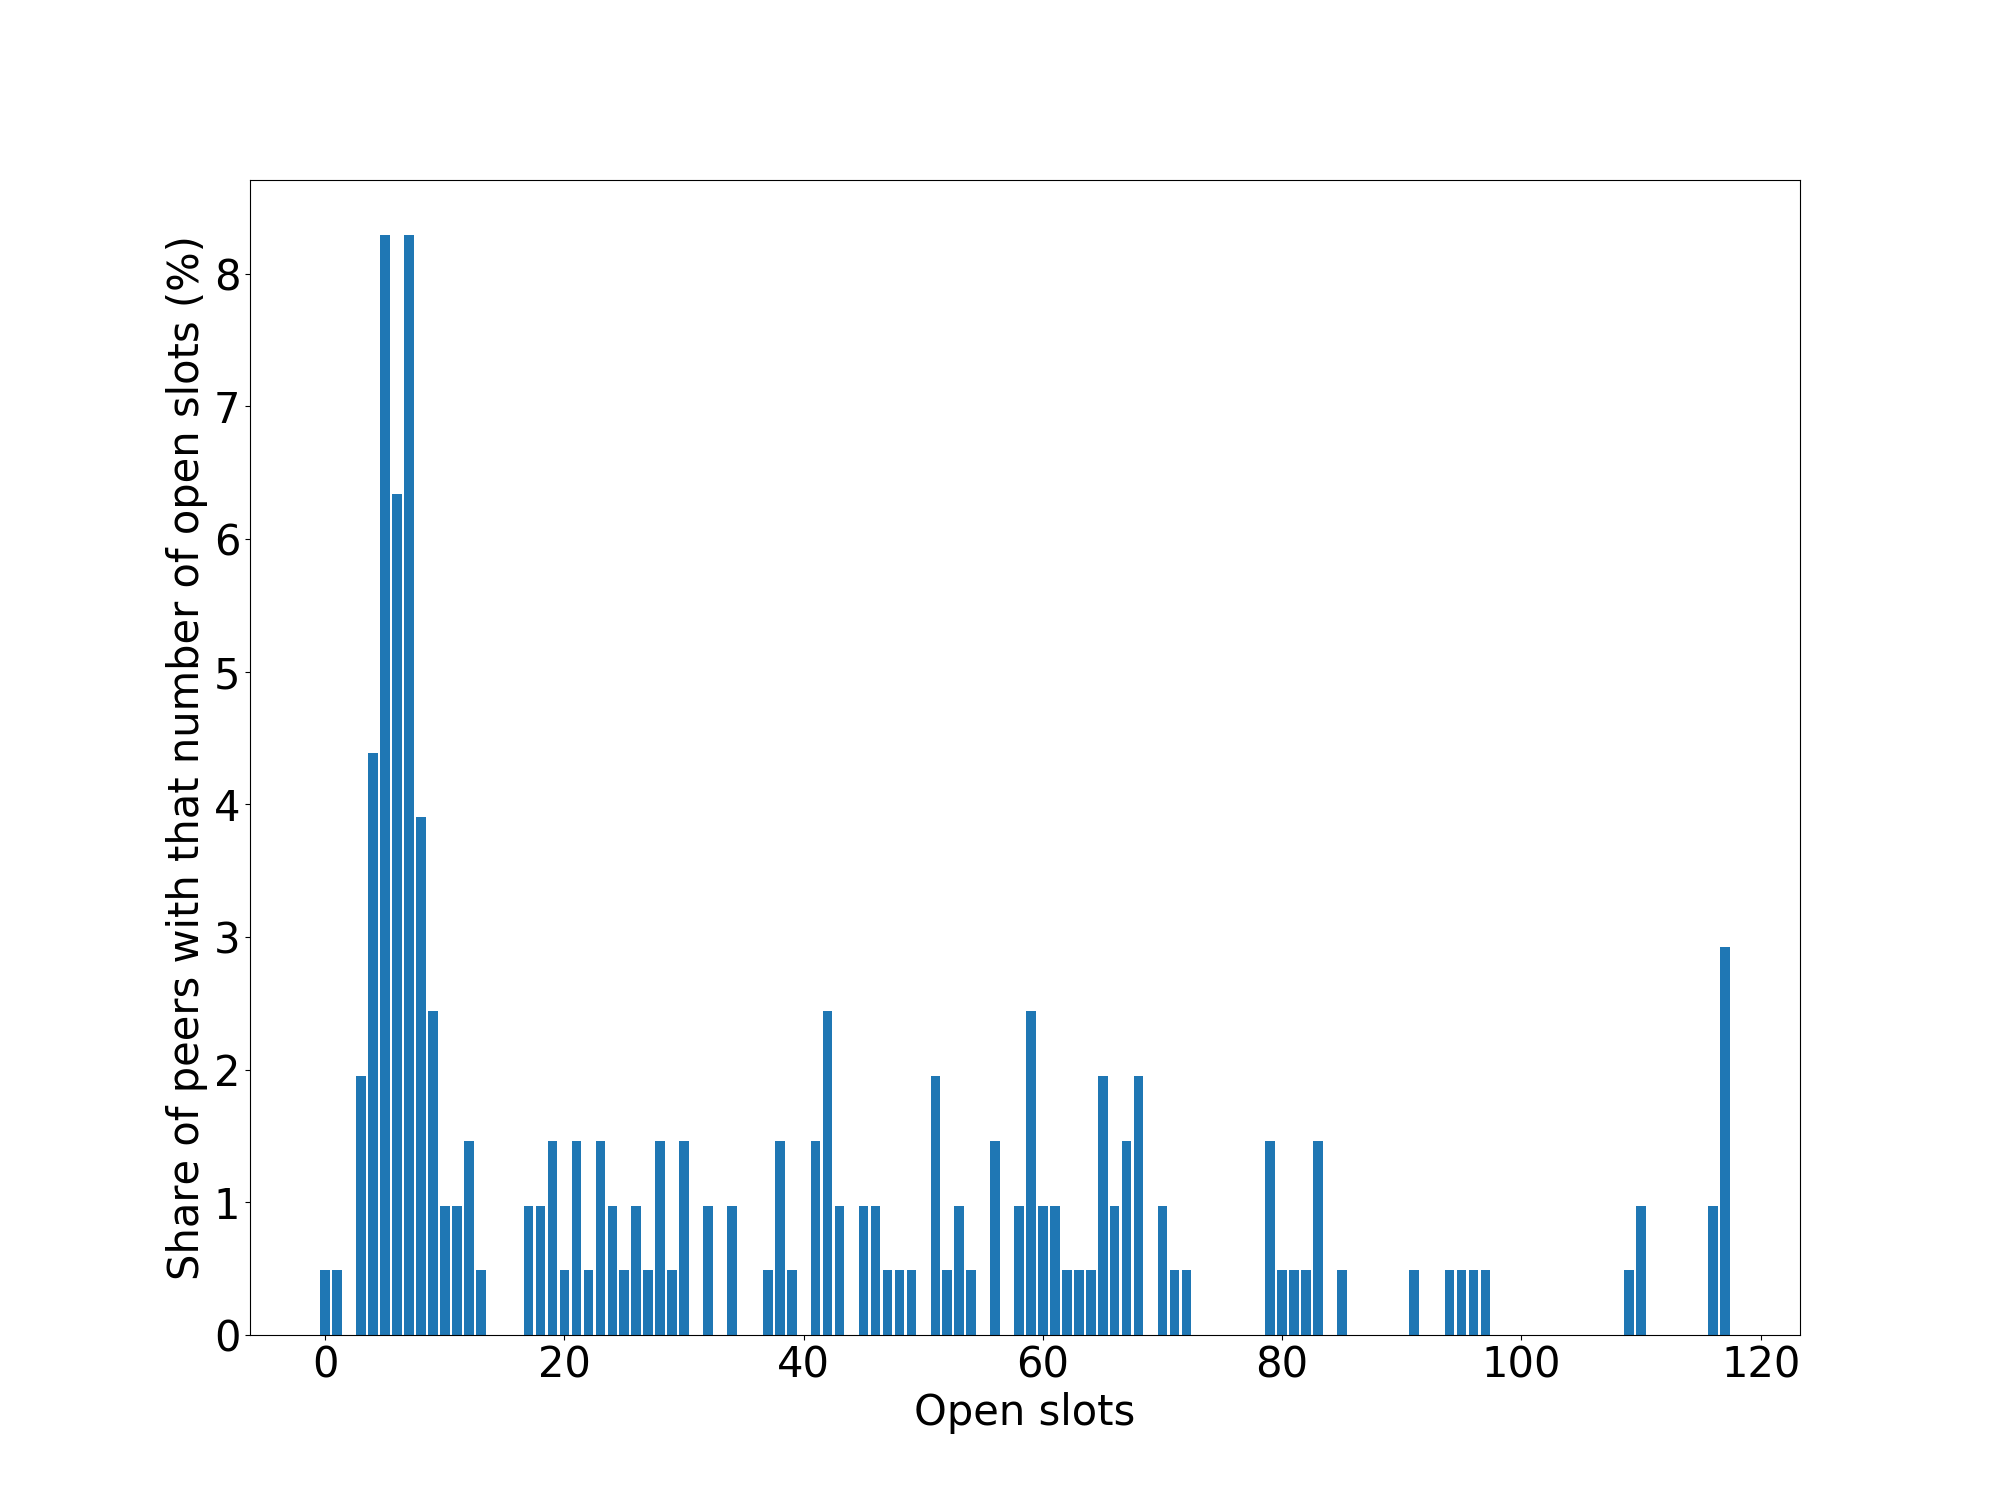
\includegraphics[width=\columnwidth]{zcash-mainnet-1541938472-conn-max-histogram.png}
		\caption{Free slots: Zcash mainnet}
	\end{minipage}\hfill
	\label{fig:free-slots}
\end{figure*}

Note that our attack does does not take into account transaction content or type.
Consequently, our method applied for Zcash allows clustering transactions involving both transparent and shielded addresses (transactions from the control set which involve shielded addresses are marked with longer ticks in the figure).


\subsubsection{Dash}

We ran an experiment on the Dash mainnet (connecting to 500~random nodes from the total of~3065, asking for 30~slots).
In addition to announcing transactions and blocks, Dash uses the inventory mechanism for managing the masternode network~\cite{Schinzel2015}, which includes periodic pings of masternodes to check whether they are functioning, managing mixing transactions, voting for governance proposals, etc.
Our tool is not yet adapted for handling Dash-specific messages.
The logs show many Dash-specific inventory messages, which do not later appear on block explorers (i.e.,~are not usual transactions).
In a 15-minute experiment we received  12~transaction inventory messages and 396~Dash-specific messages.
% this is weird: 9-10 July 2018 there was 8-10k tx / day = avg 90+ for 15-min window, we got 12
% most probably, mixed txs are broadcast with another message type
We ran our clustering algorithm two times: taking Dash-specific messages into account (Figure~\ref{fig:dash-all}), and considering only usual transaction inventory messages (Figure~\ref{fig:dash-tx}).

\begin{figure}[!t]
	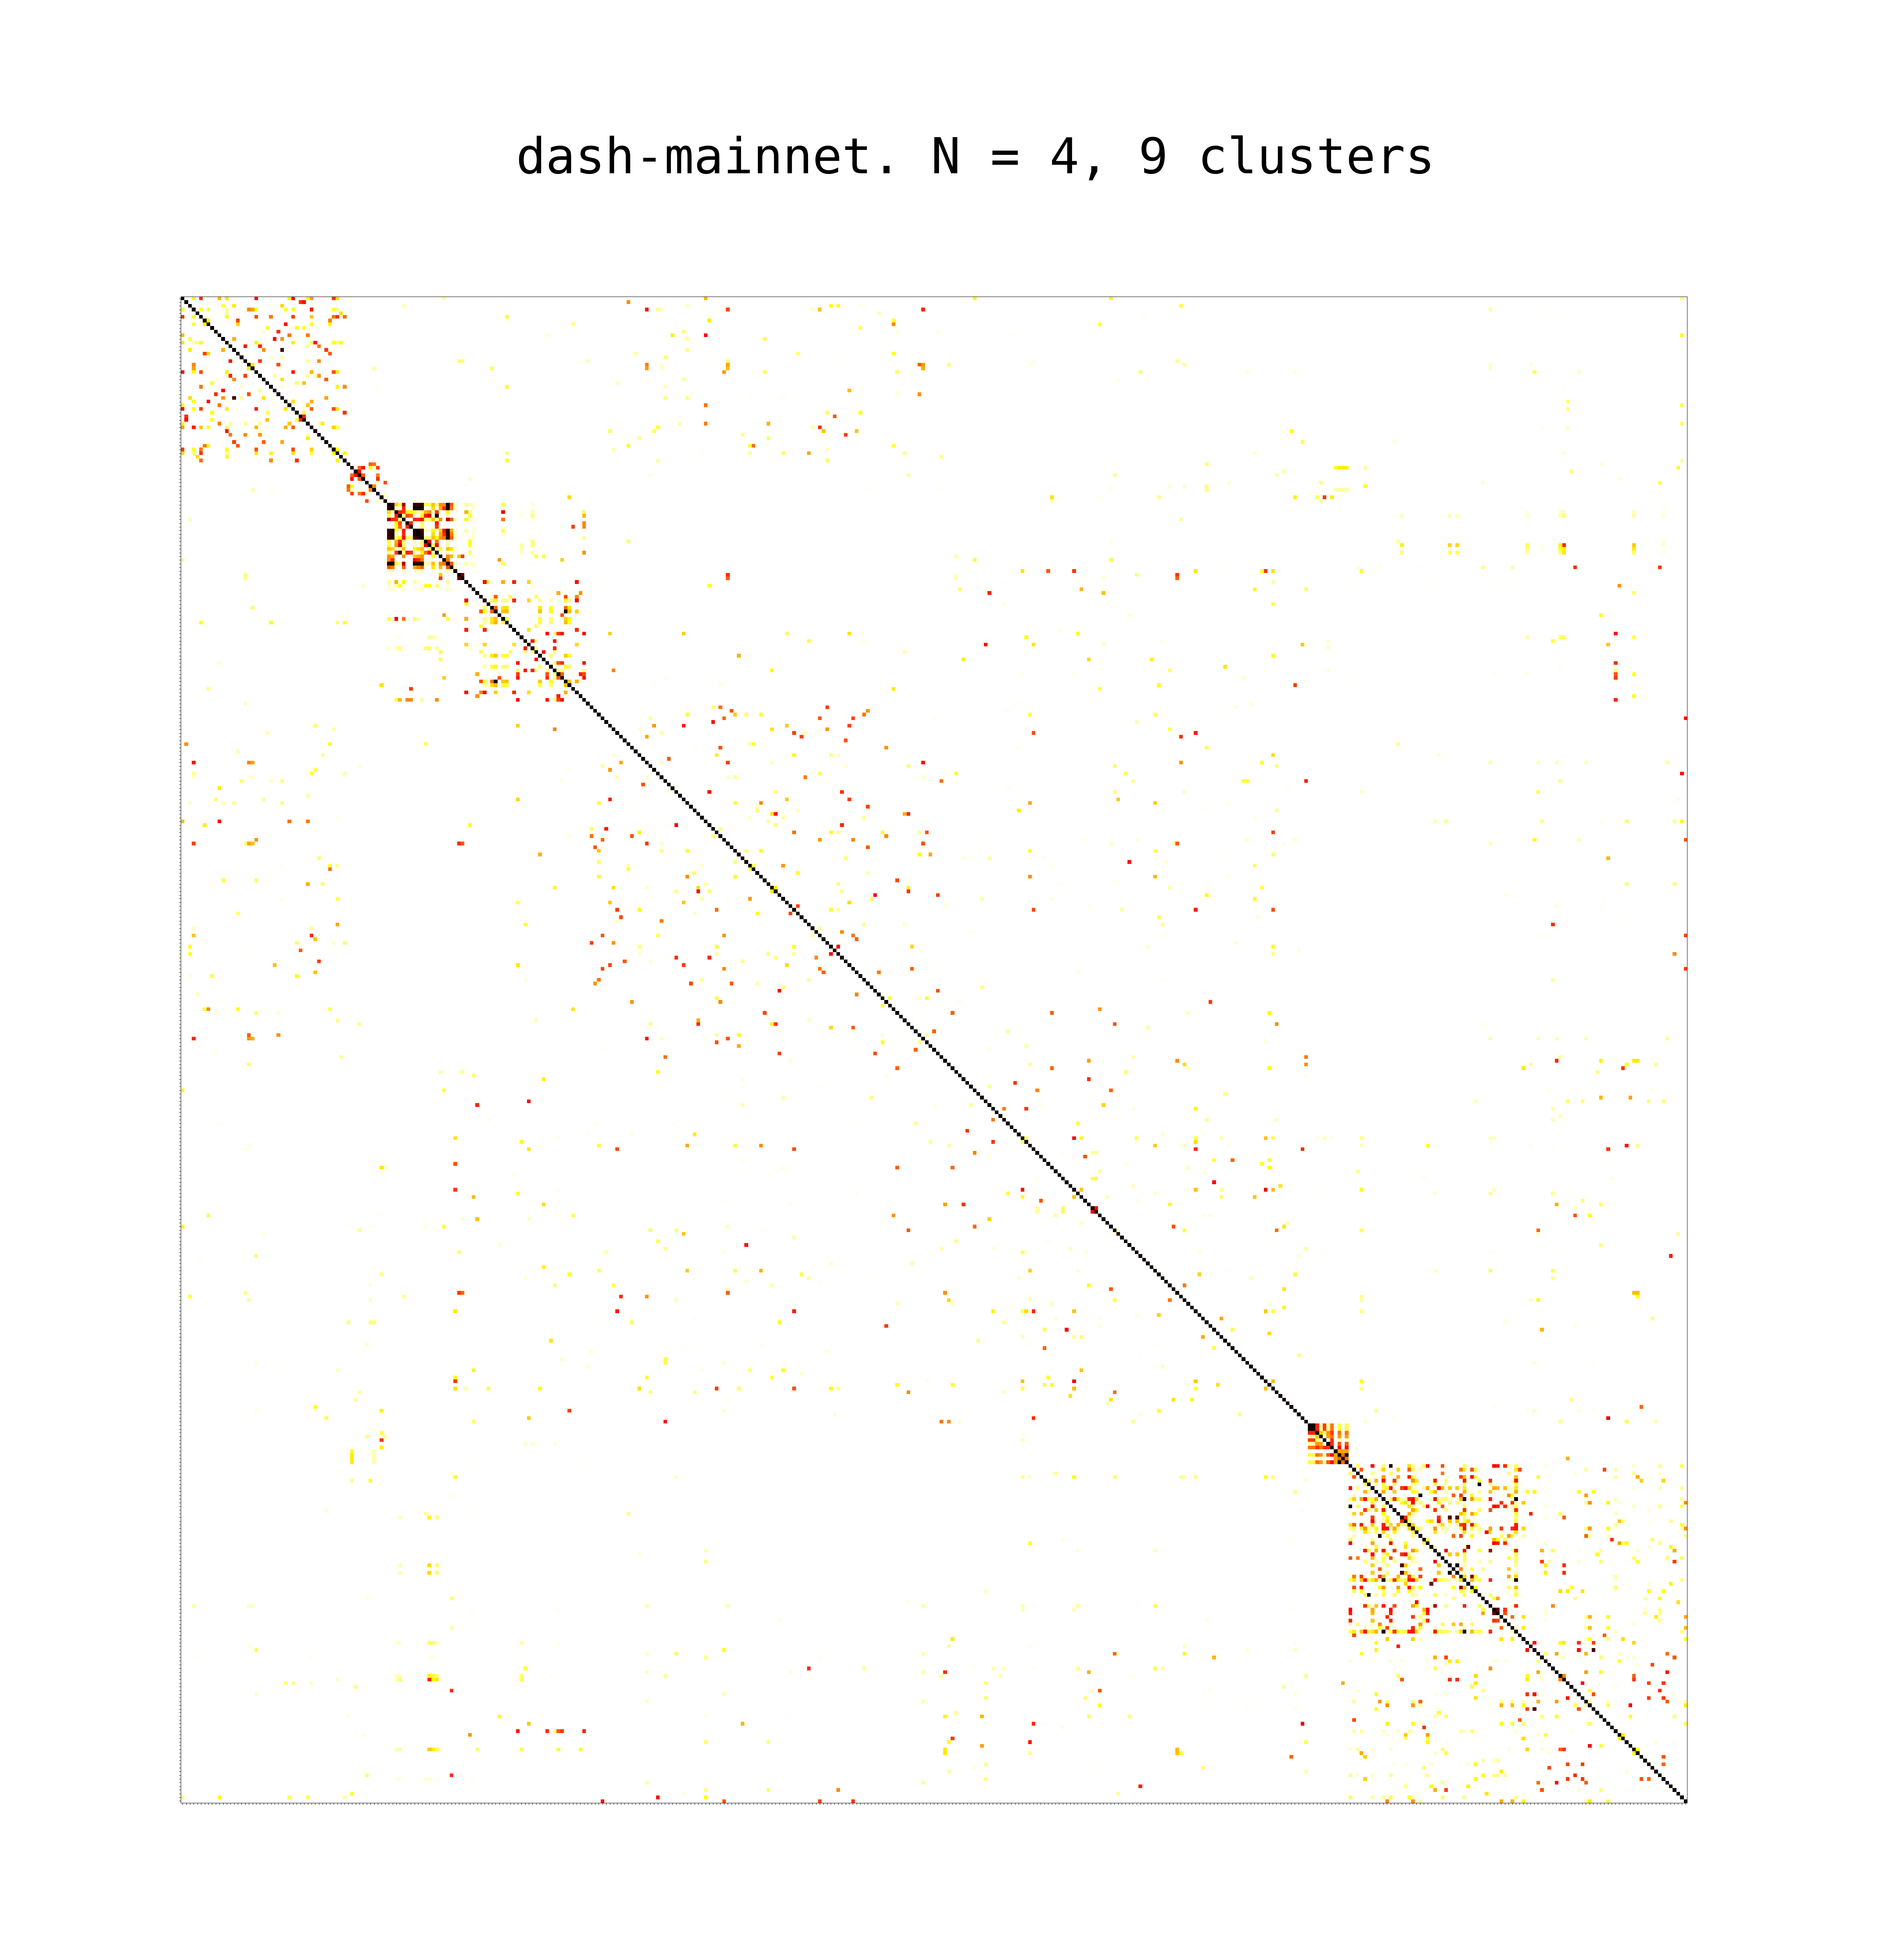
\includegraphics[width=\columnwidth]{dash-mainnet-1531510768-all.png}
	\caption{Dash (Dash-specific messages and usual transactions)}
	\label{fig:dash-all}
\end{figure}

\begin{figure}[!t]
	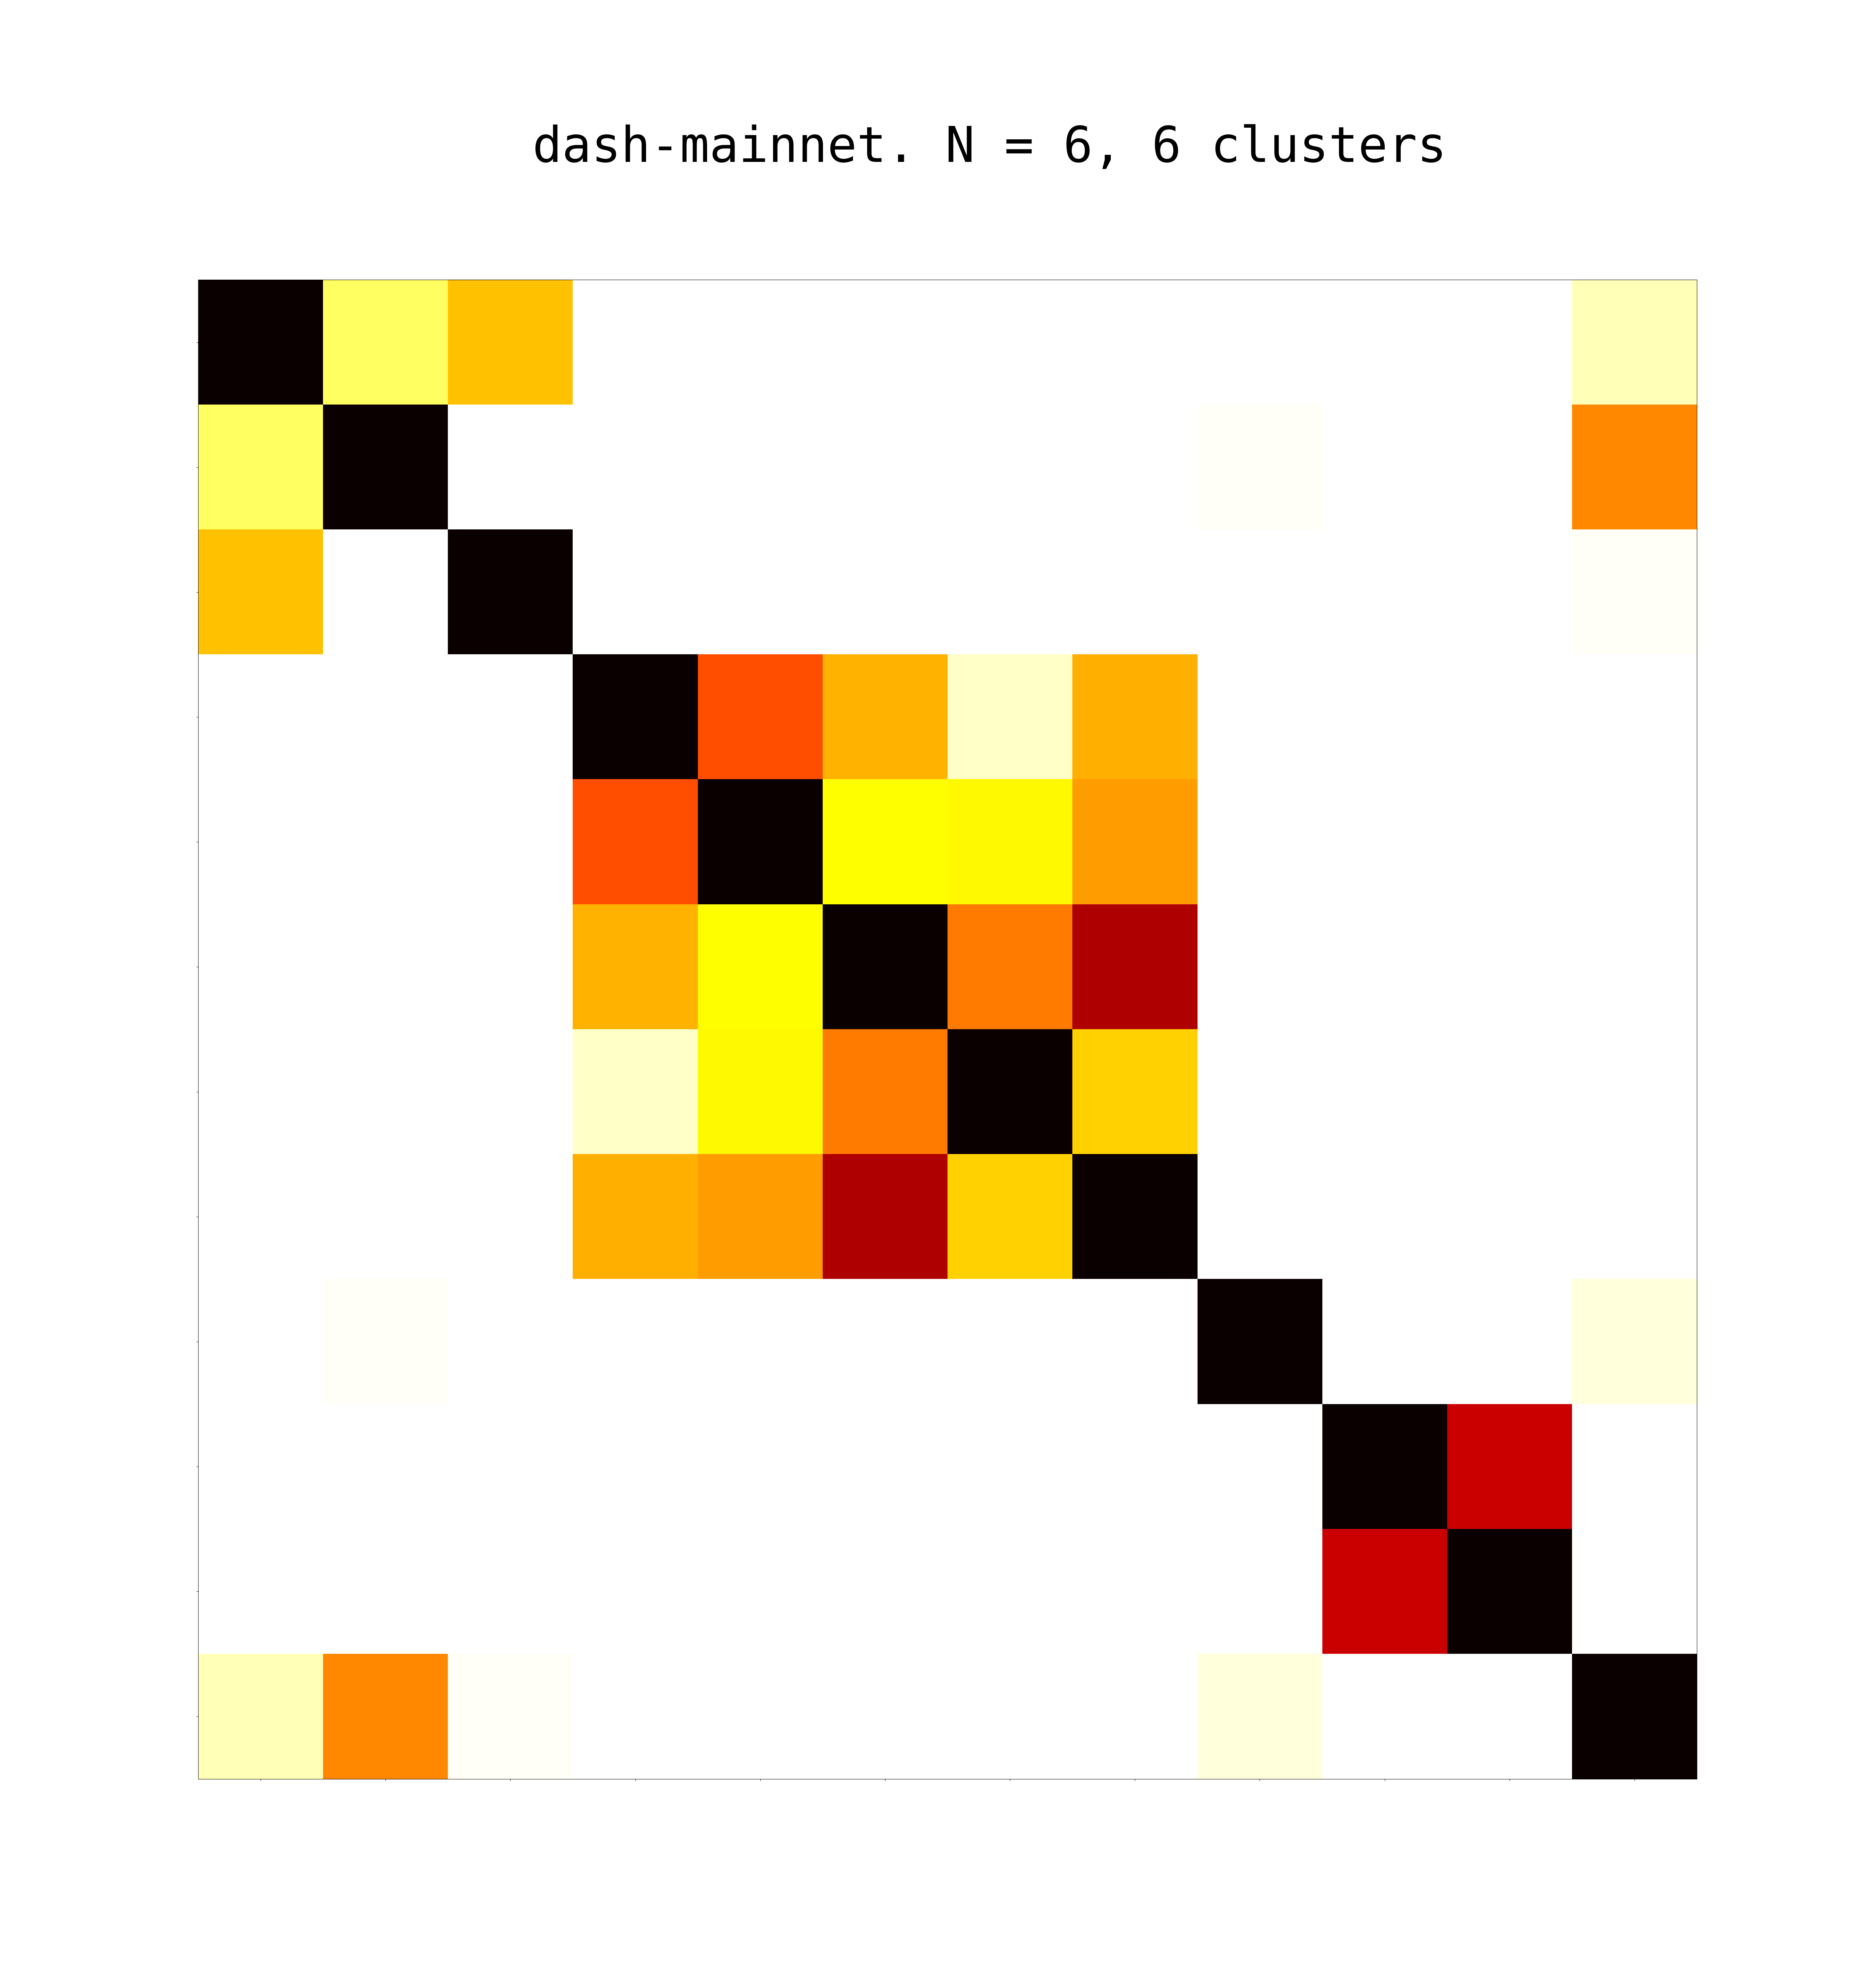
\includegraphics[width=\columnwidth]{dash-mainnet-1531510768.png}
	\caption{Dash (usual transactions)}
	\label{fig:dash-tx}
\end{figure}

In both cases, we obtained clearly visible clusters.
These preliminary results demonstrate a clear privacy concern, especially if network analysis is combined with deanonymization attacks on Dash based on transaction graph analysis~\cite{Kalodner2017}. 
%clear target for future research


\subsubsection{Monero}

Contrary to Bitcoin, that allows spending a transaction output before it is confirmed, Monero imposes certain restrictions.
A new output appears as "locked" until the corresponding transaction gets 10~confirmations (20~minutes at the target block time of 2~minutes)~\cite{dpzz2017}.
Though this is a wallet-level restriction and not a protocol-level one, the major implementations (the official desktop wallet and Monerujo wallet for Android) support it.
This means that the scenario of our previous experiments is rather unrealistic: for example, in order to issue 20~transactions within a 20~minute period, a user must have 20~independent, "unlocked" transaction outputs (each of which takes 20~minutes to create).

Further inspection of the source code and an answer on a Monero-related Q\&A site reveals that Monero nodes do not limit the number of incoming connections by default~\cite{user363032016}.
Monero is the only one of the three privacy-preserving currencies which is private by default: users do not have to explicitly choose the "private" option (such as a shielded address in Zcash and PrivateSend in Dash).
In October~2018, Monero version 0.13.0 introduced an implementation of Bulletproofs -- a cryptographic technique which allowed greatly reduced transaction size (and hence fees), which also, similar to Sapling in Zcash, is expected to incentivize Monero adoption on devices with limited resources~\cite{Spagni2018}.

We check the suitability of our technique on Monero by performing an experiment without our own transactions.
The goal of the experiment is to check whether we observe a block-diagonal structure of the correlation matrix between transaction propagation vectors.

We connected to 200 nodes (with a single connection per node) and received 124~transactions in a 38~minute window (see Figure~\ref{fig:monero}).

\begin{figure}[!t]
	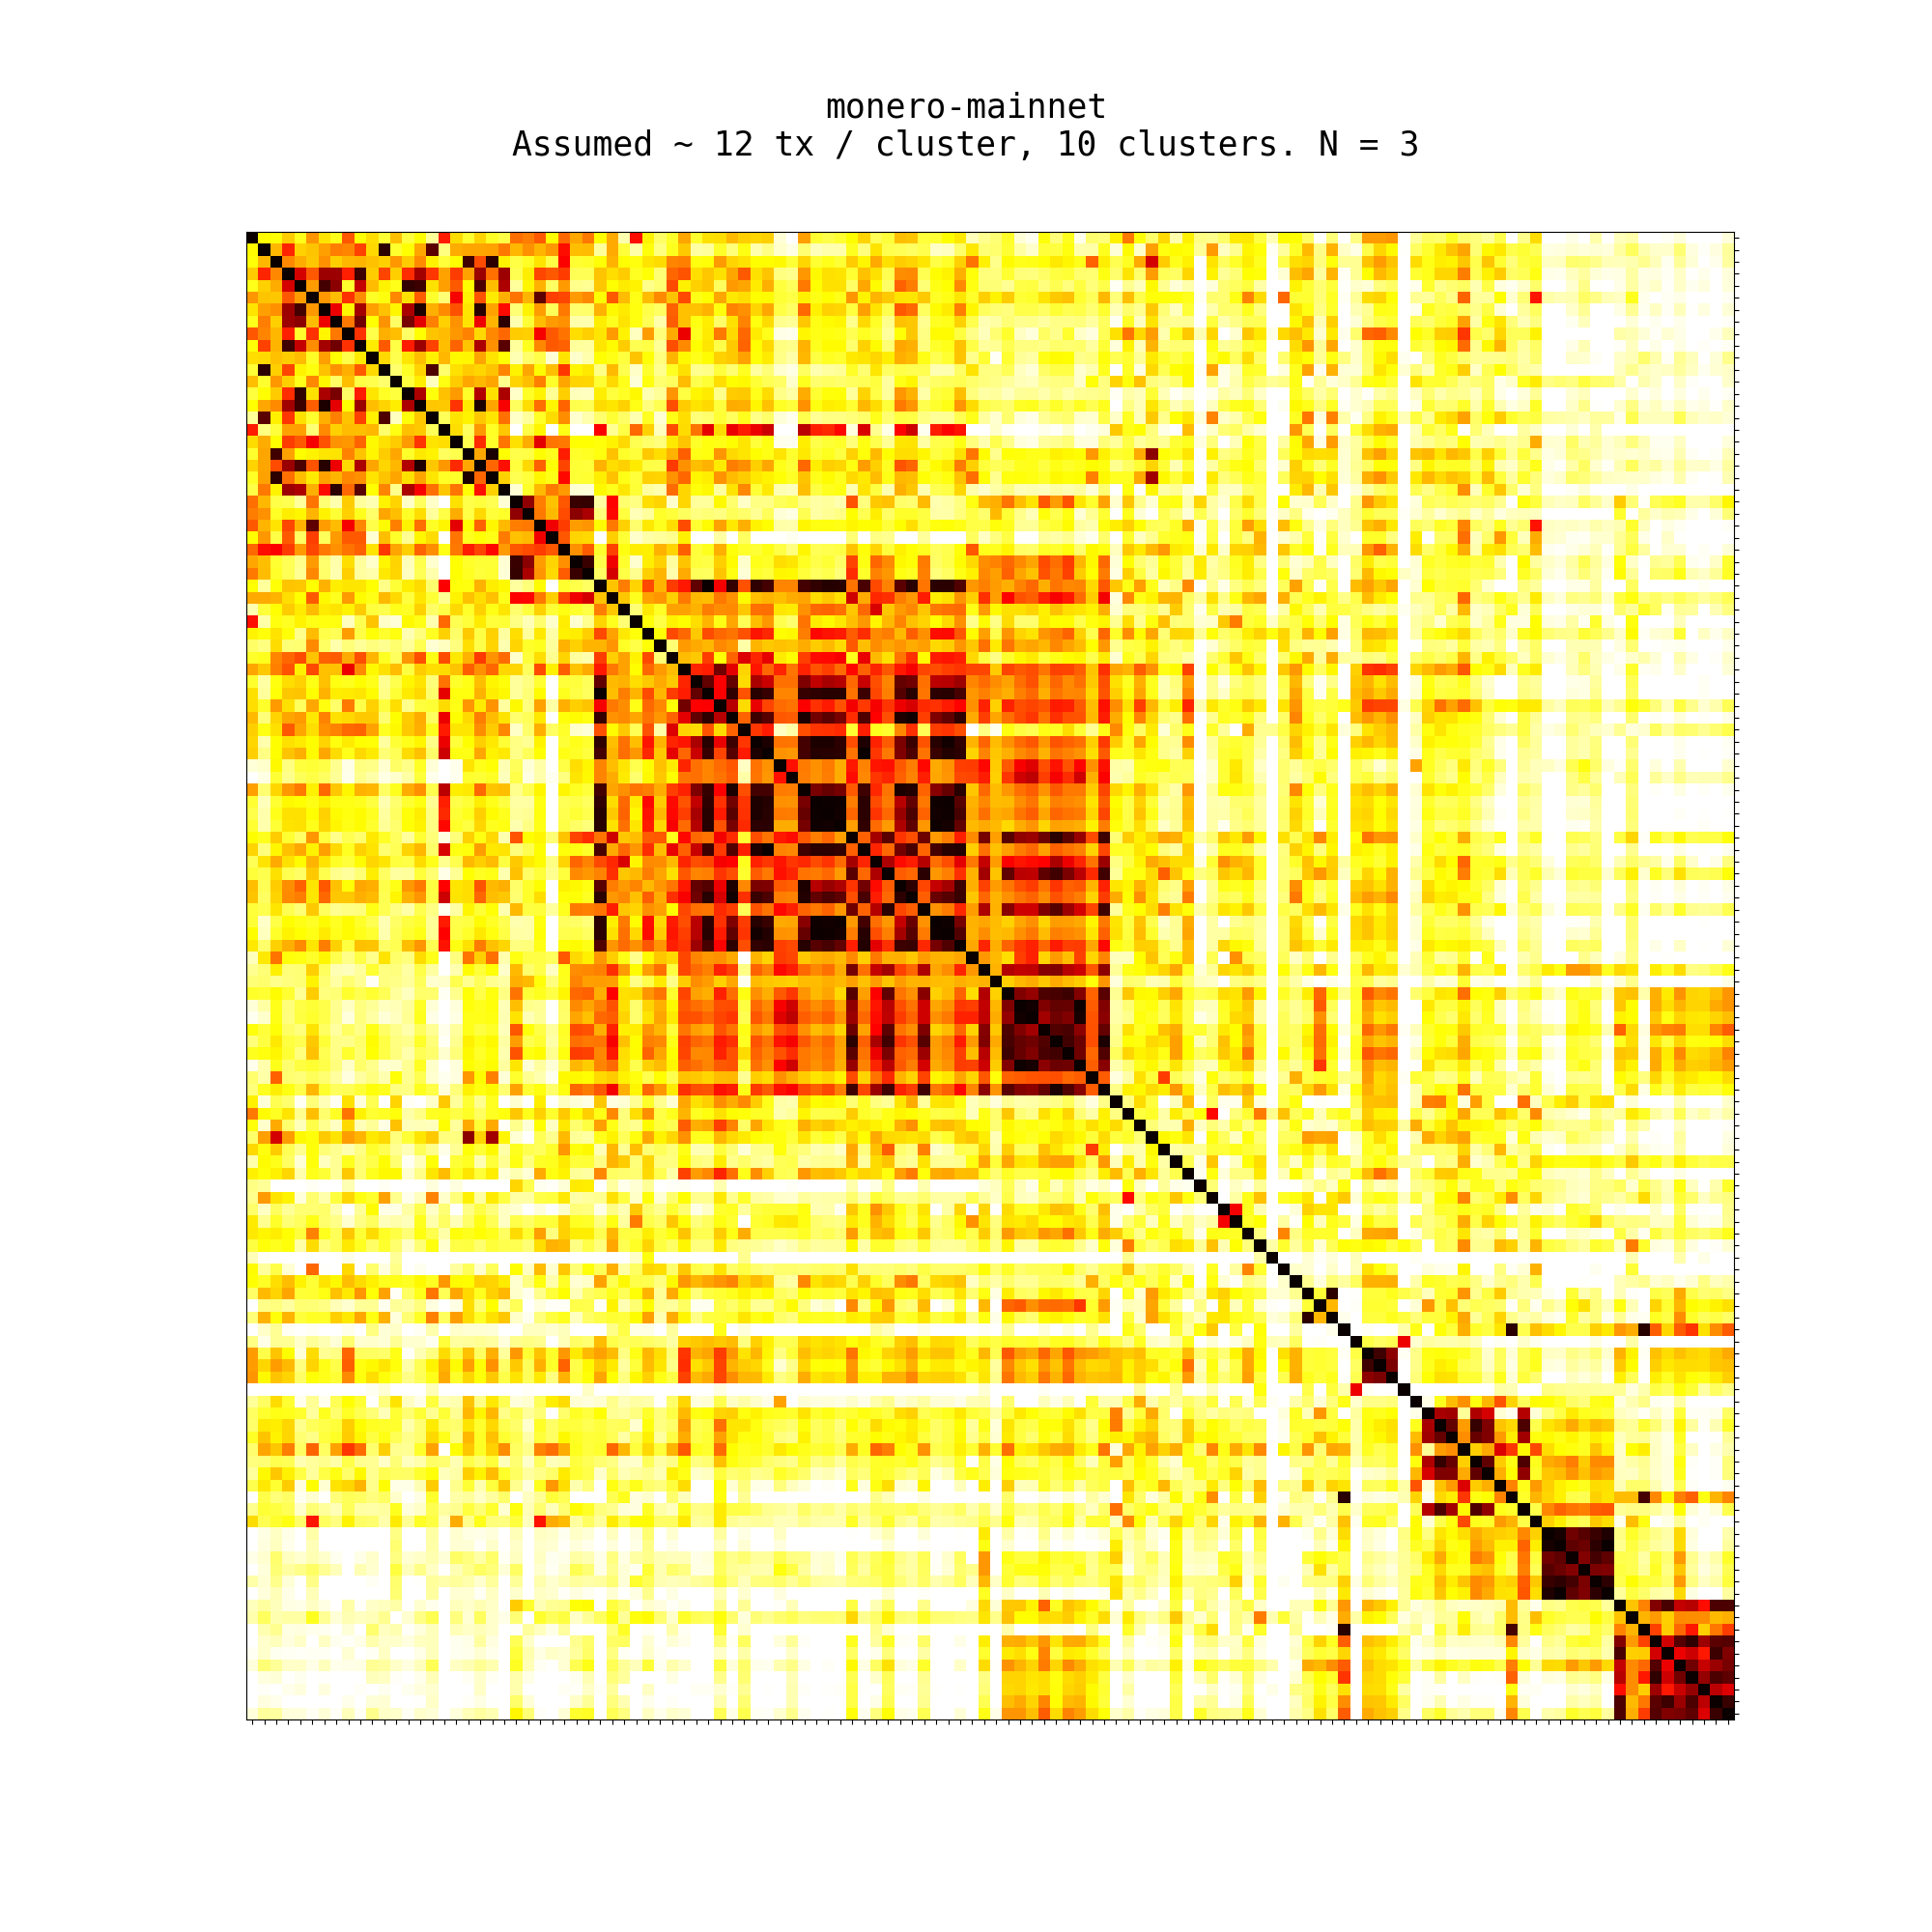
\includegraphics[width=\columnwidth]{monero-mainnet-005-fig-correlations-012-txcl-003-N-Rand-best.png}
	\caption{Monero}
	\label{fig:monero}
\end{figure}

The less clear picture compared to e.g.~Bitcoin testnet may be explained as follows:
\begin{itemize}
	\item We establish connections with too few nodes (200, while the total number of nodes is estimated at 1700-1800~\cite{MoneroHash});
	\item The propagation mechanism is not optimized: there is no \texttt{INV} -- \texttt{GETDATA} -- \texttt{TX} exchange, transactions are relayed unconditionally to all neighbors, which blurs the picture. On the other hand, an adversary connecting to nearly all nodes is expected to gain a near-perfect insight into the original broadcasters of transactions, as IP addresses of transaction authors will most likely be among the first to relay a transaction to the adversary.
\end{itemize}
Another peculiarity which makes our analysis more difficult is that \texttt{monerod} connects to nodes relatively slowly (compared to \texttt{bcclient}).
In our experiment, while trying to connect to 200~nodes, we got 150~connections only after approximately 2~hours, 175~connections after 3~hours, 200~connections after nearly 8~hours.
We also notice that none of the hard-coded DNS seeds resolves (as of mid-July~2018); the client falls back to seed IP addresses (also hard-coded).


\subsection{Results for mobile wallets}

We also performed analogous experiments on selected mobile wallets.
\footnote{Chapter~\ref{Chapter04Wallets} is dedicated to evaluating other privacy-related aspects of mobile cryptocurrency wallets.}

We considered a number of wallets for Android.
\footnote{The full list and privacy analysis is presented in Chapter~\ref{Chapter04Wallets}.}
Most wallets connect to the P2P network indirectly via a trusted server maintained by the wallet's developers.
From the wallets that connect to the P2P network directly (we refer to them as P2P wallets), most rely on the BitcoinJ library for networking.
None of them uses randomizes broadcasts with diffusion or trickling.
Unlike Bitcoin~Core, BitcoinJ sends \texttt{TX} unconditionally\footnote{Note that in this case a full node receiving a \texttt{TX} message from an SPV node can be sure that the transaction originated at that SPV node whereas receiving an \texttt{INV} announcement from a full node may also be a re-broadcast. This demonstrates the privacy enhancement of exclusively connecting to a trusted node for SPV.}.
The BitcoinJ developers acknowledge that the three-step \texttt{INV} -- \texttt{GETDATA} -- \texttt{TX} exchange in Bitcoin~Core improves privacy, but argue that since BitcoinJ is used by light nodes with a priori weaker privacy guarantees, the three-step broadcast would only decrease efficiency.
BitcoinJ and BRD broadcast a new transaction to a subset of entry nodes and wait for the announcement from other ones, which is taken as a sign of network acceptance.

We focus on three networks for our experiments: Bitcoin testnet, Bitcoin mainnet, and Zcash mainnet.
Bitcoin testnet is the most active testnet of an open cryptocurrency and is a perfect testing ground to perform fully-fledged experiments.
We test the applicability of our technique on the two mainnets while not aiming to fully occupy the connection slots to avoid impacting the real networks.
For the experiments we choose popular wallets with well-established brands (both Bitcoin-only and multi-coin), with centralized as well as P2P broadcast mechanisms.

Our tool is not fully compatible with Dash and Monero.
Dash, while based on a fork of Bitcoin~Core, introduces many additional message types to manage the masternode network.
Monero is implemented independently and uses another networking mechanism, although based on the same principles.

For centralized wallets, instead of issuing two sets of transactions, we only issue one set, using it as a "label" for a presumed wallet cluster.
If our transactions form a visible cluster, we inspect the IP addresses of nodes which were among the first ones to broadcast them and assume those are the wallet nodes.
This allows us to infer the IP addresses of nodes which a wallet uses for transaction broadcasts.
We can then associate transactions in the network with popular wallets.
%We also do not log \texttt{ADDR} messages: they are only useful in deanonymizing P2P wallets.

\begin{figure}
	\centering
	\begin{subfigure}{.5\textwidth}
		\centering
		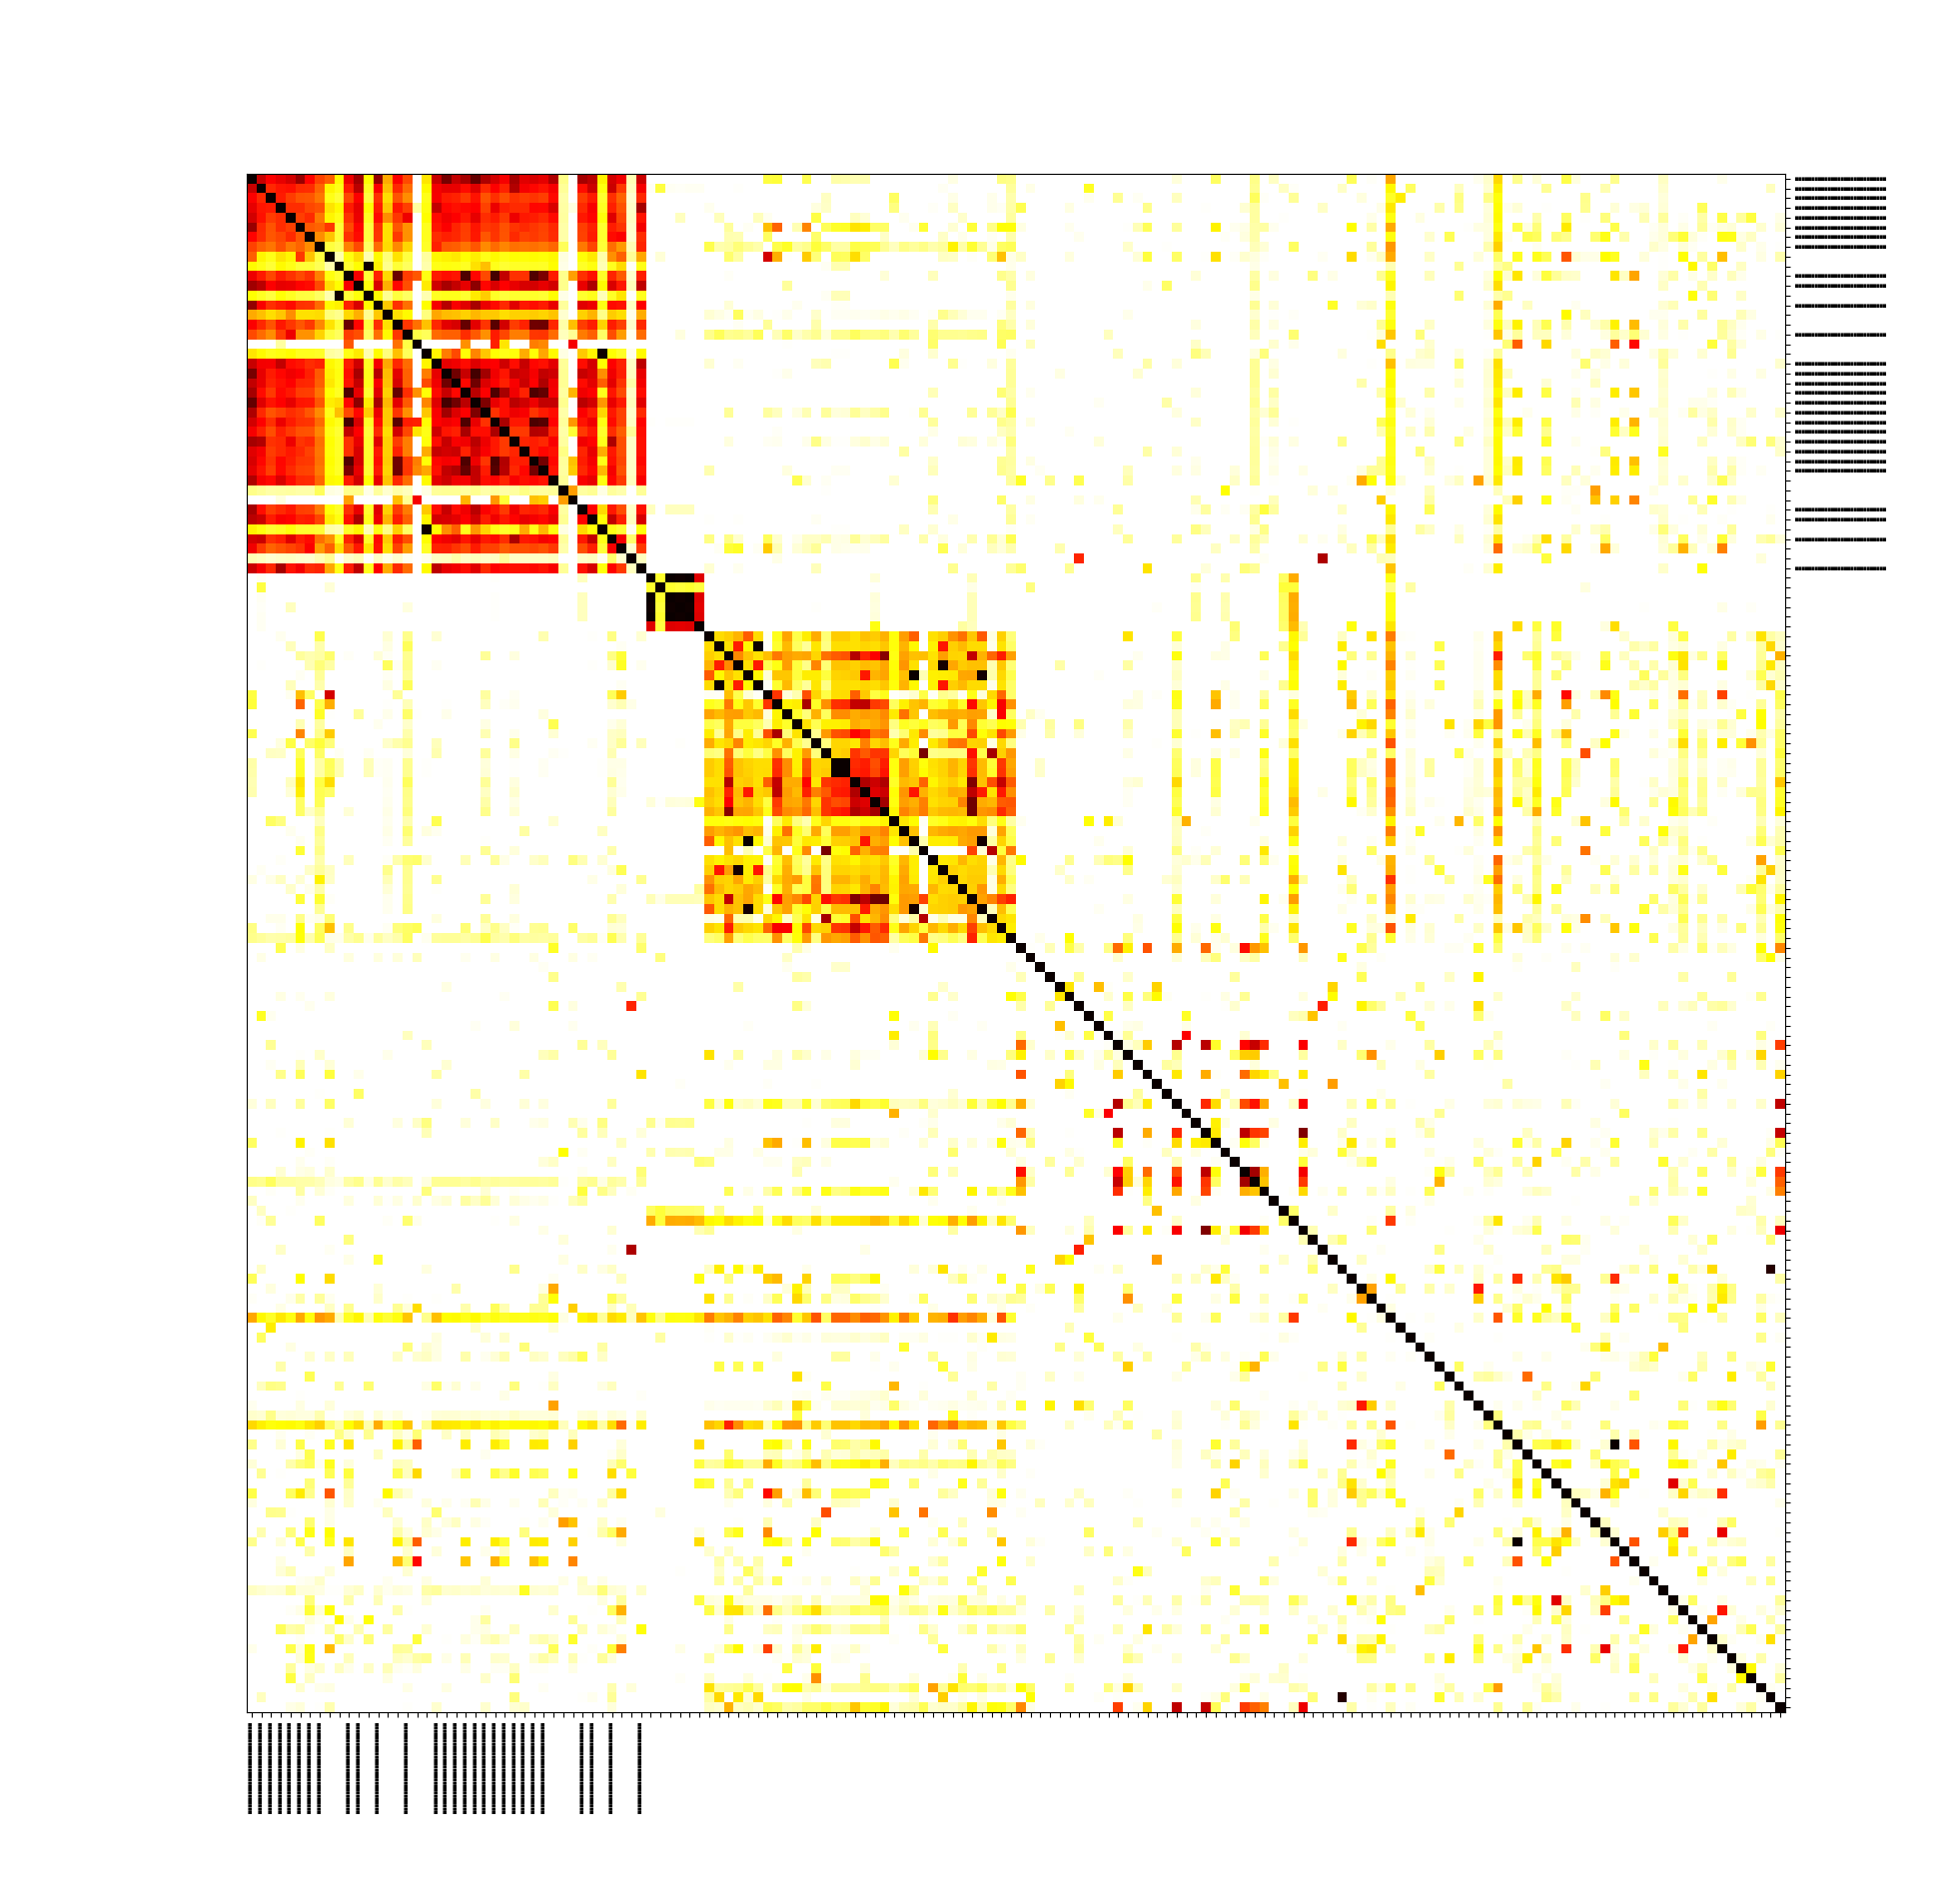
\includegraphics[width=\columnwidth]{bitcoin-testnet-1542895555-fig-corr-032-txcl-005-N-Rand.png}
		\caption{Mycelium (testnet)}
	\end{subfigure}%
	\begin{subfigure}{.5\textwidth}
		\centering
		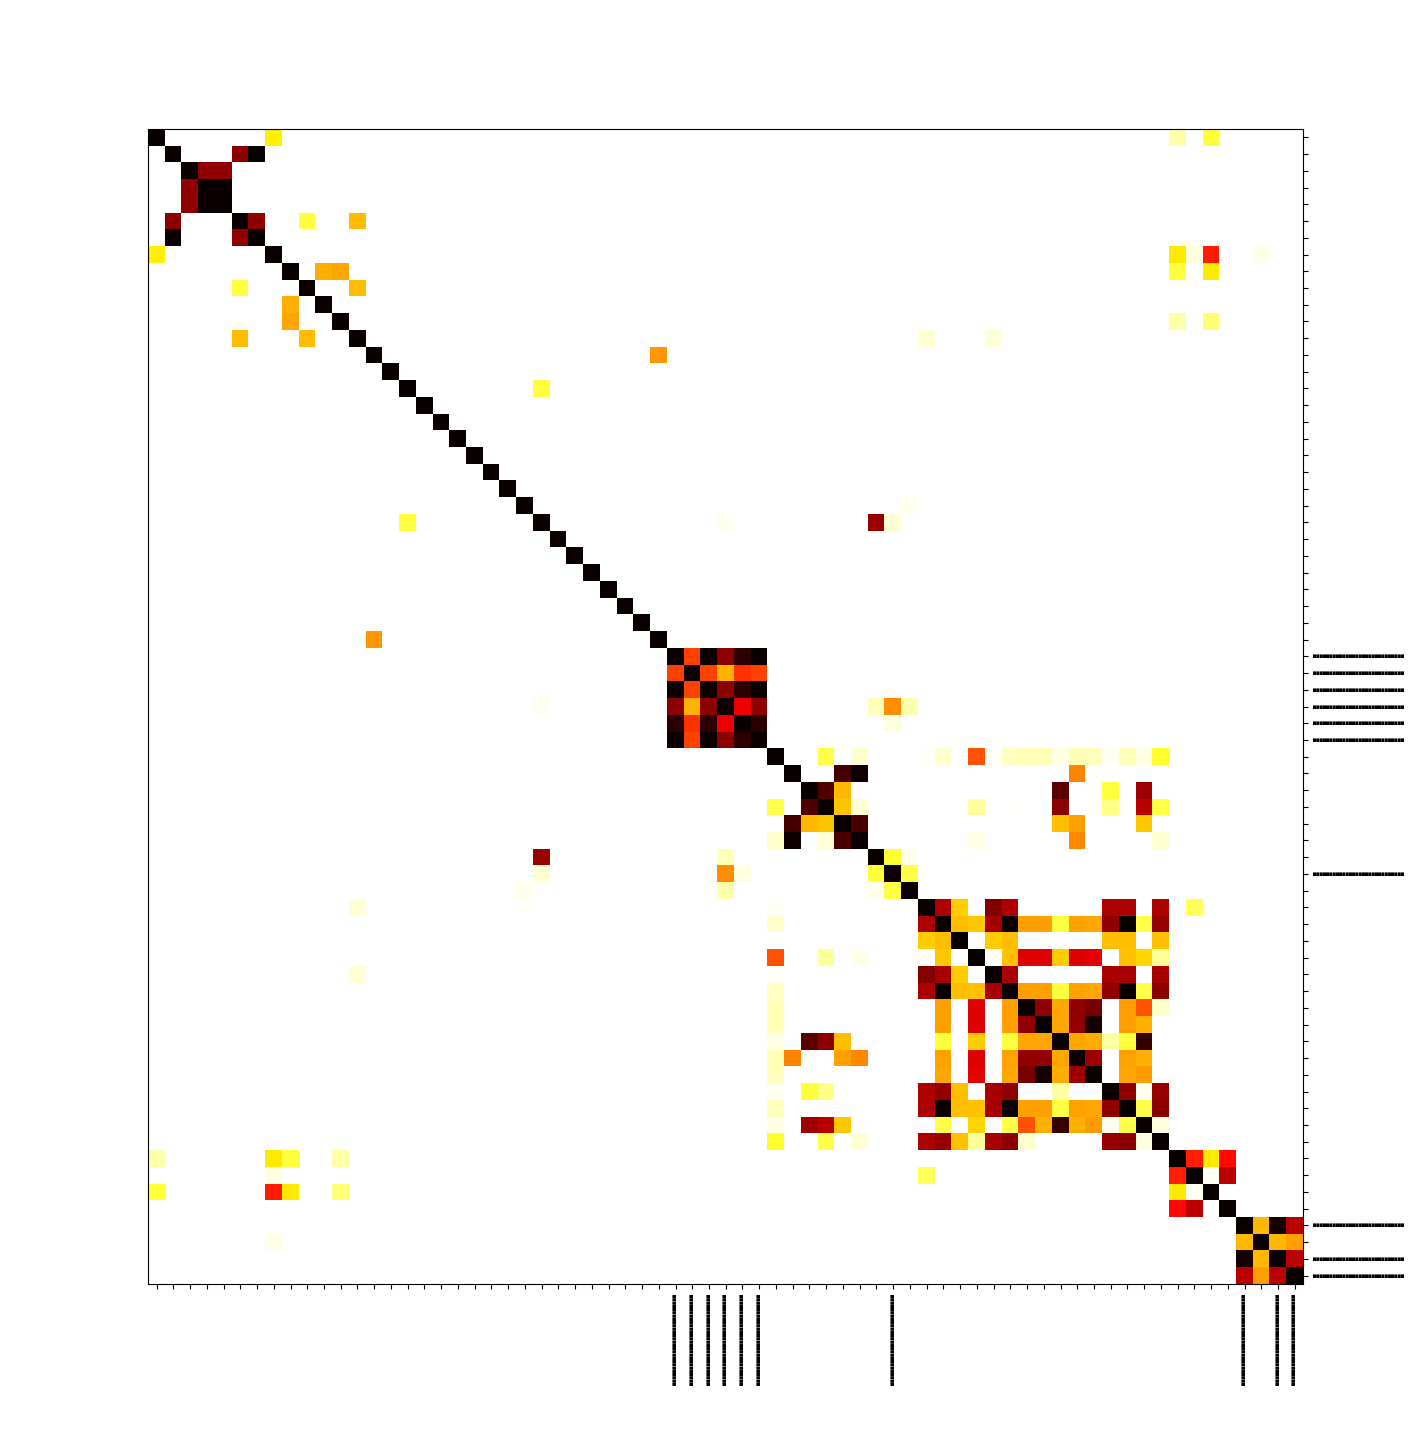
\includegraphics[width=\columnwidth]{bitcoin-testnet-1537202356-fig-corr-008-txcl-003-N-Rand.png}
		\caption{Bitcoin wallet (testnet)}
	\end{subfigure}
	\begin{subfigure}{.5\textwidth}
		\centering
		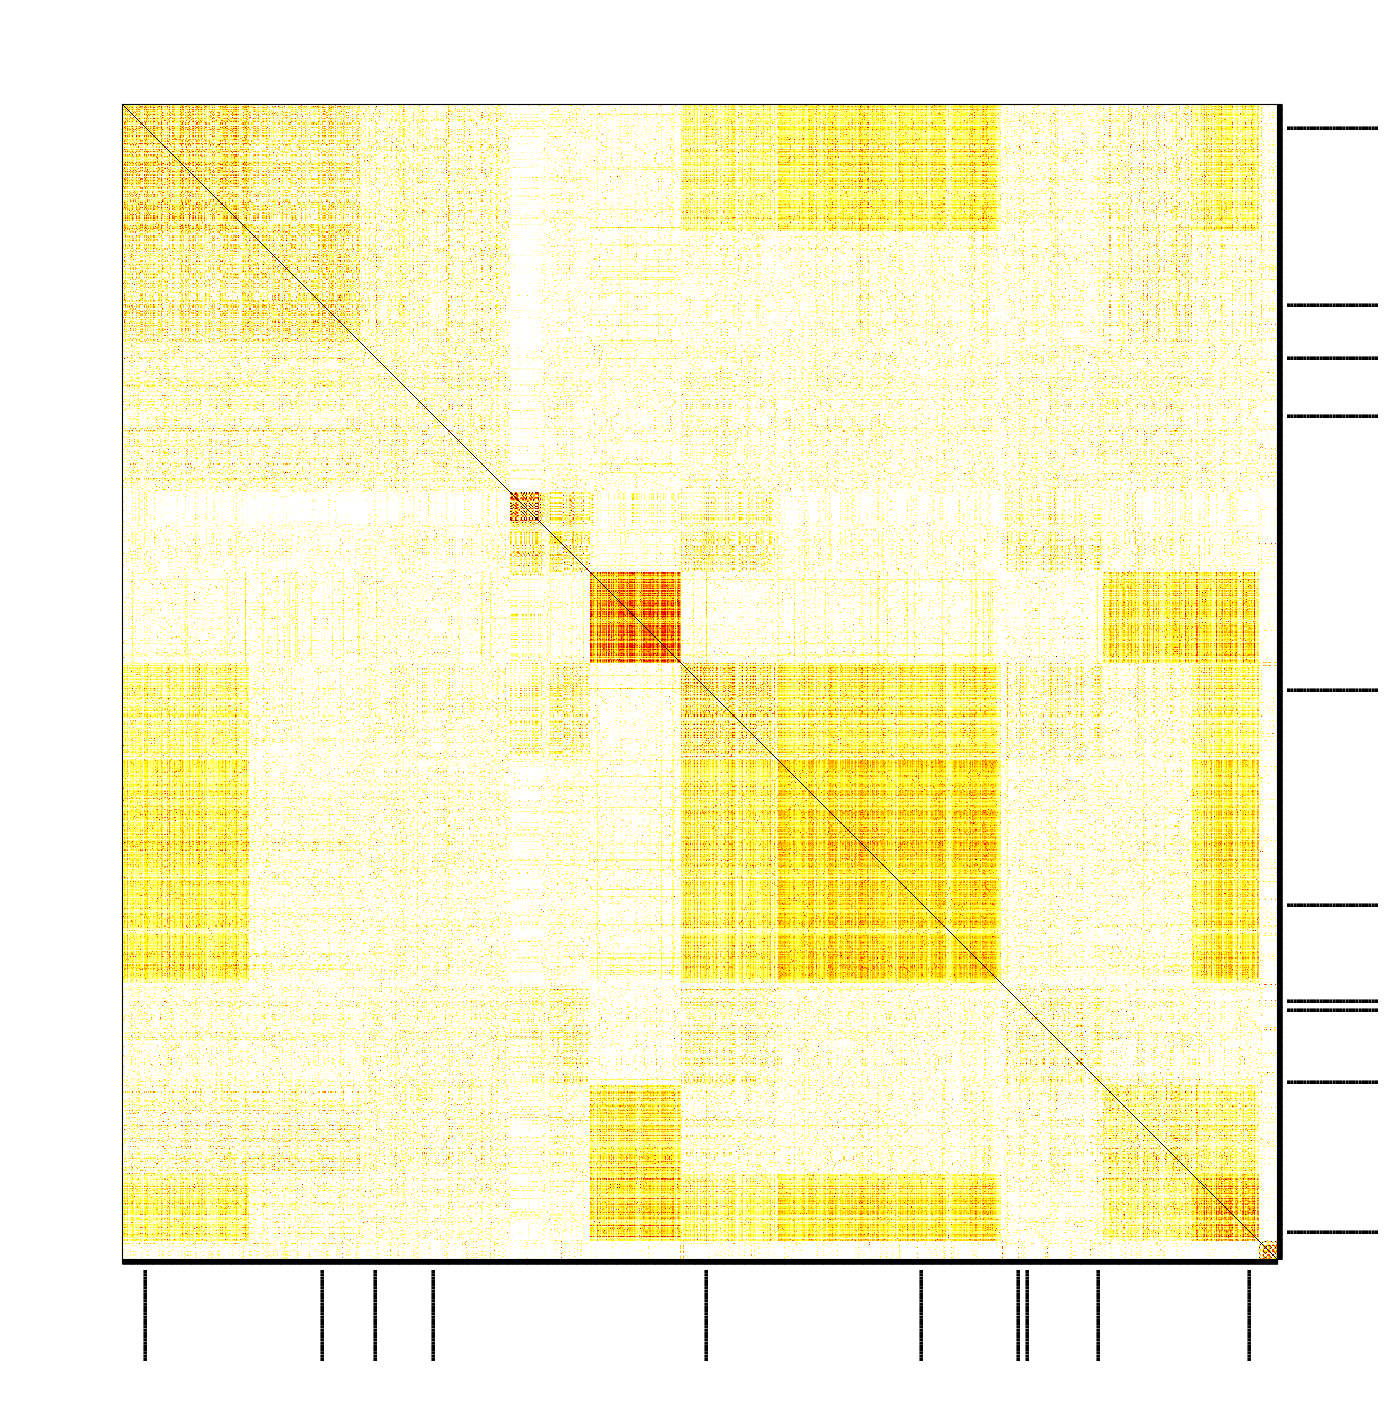
\includegraphics[width=\columnwidth]{bitcoin-mainnet-1537365306-fig-corr-202-txcl-007-N-Rand.png}
		\caption{Bitcoin wallet}
	\end{subfigure}%
	\begin{subfigure}{.5\textwidth}
		\centering
		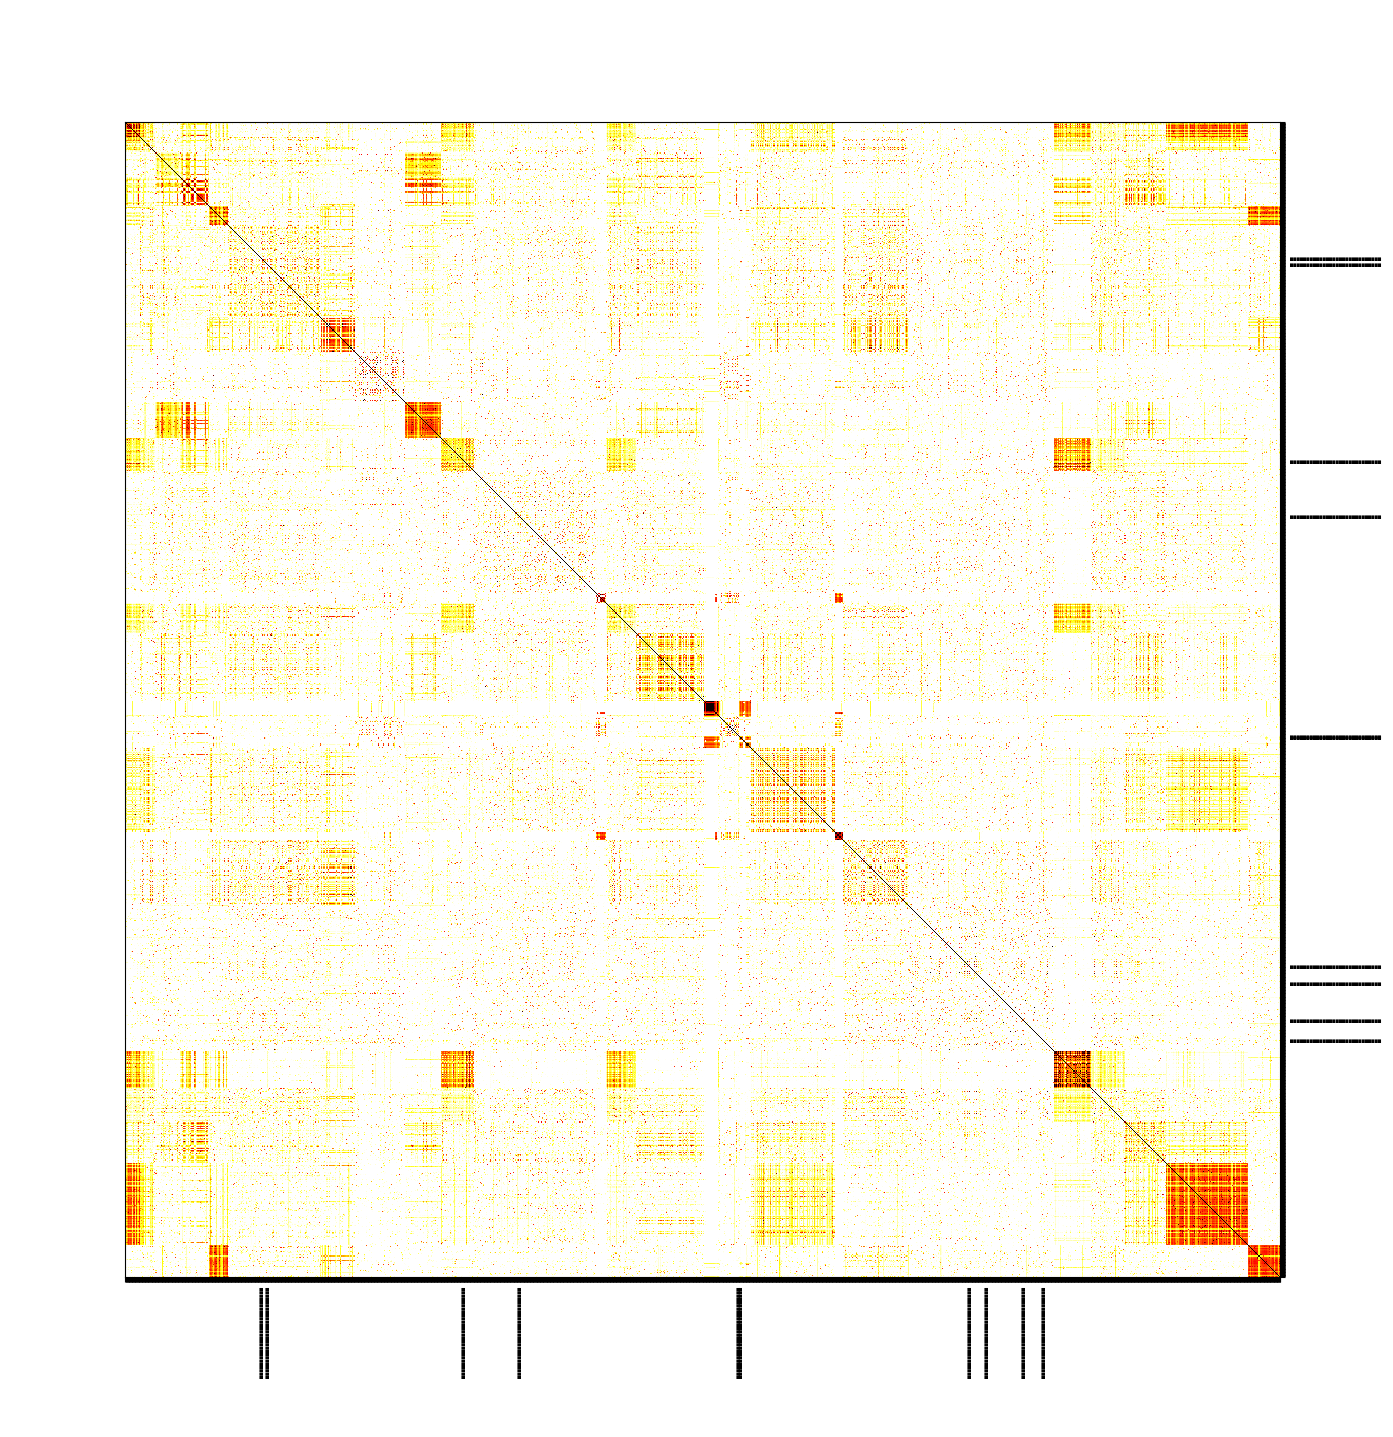
\includegraphics[width=\columnwidth]{bitcoin-mainnet-1537377559-fig-corr-102-txcl-004-N-Rand.png}
		\caption{BRD}
	\end{subfigure}
	\begin{subfigure}{.5\textwidth}
		\centering
		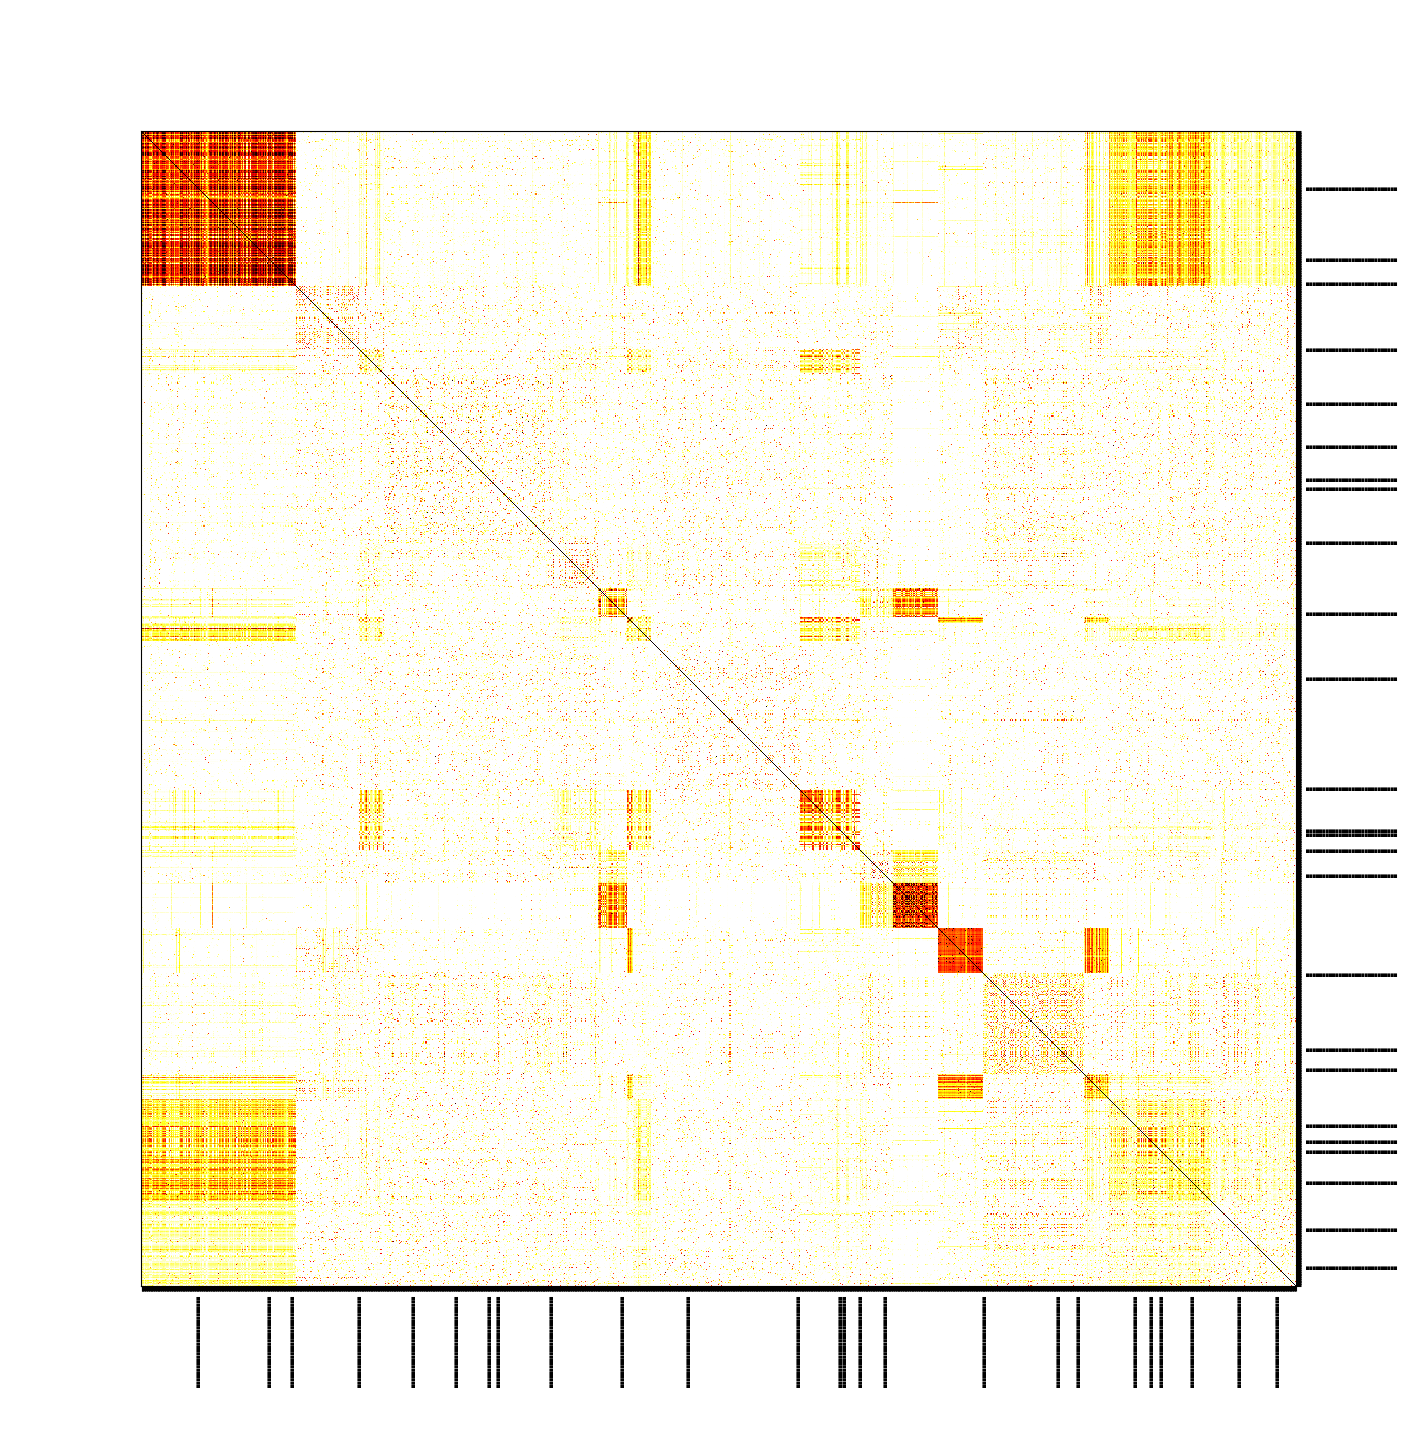
\includegraphics[width=\columnwidth]{bitcoin-mainnet-1537951300-fig-corr-100-txcl-004-N-Rand.png}
		\caption{Coinomi}
	\end{subfigure}%
	\begin{subfigure}{.5\textwidth}
		\centering
		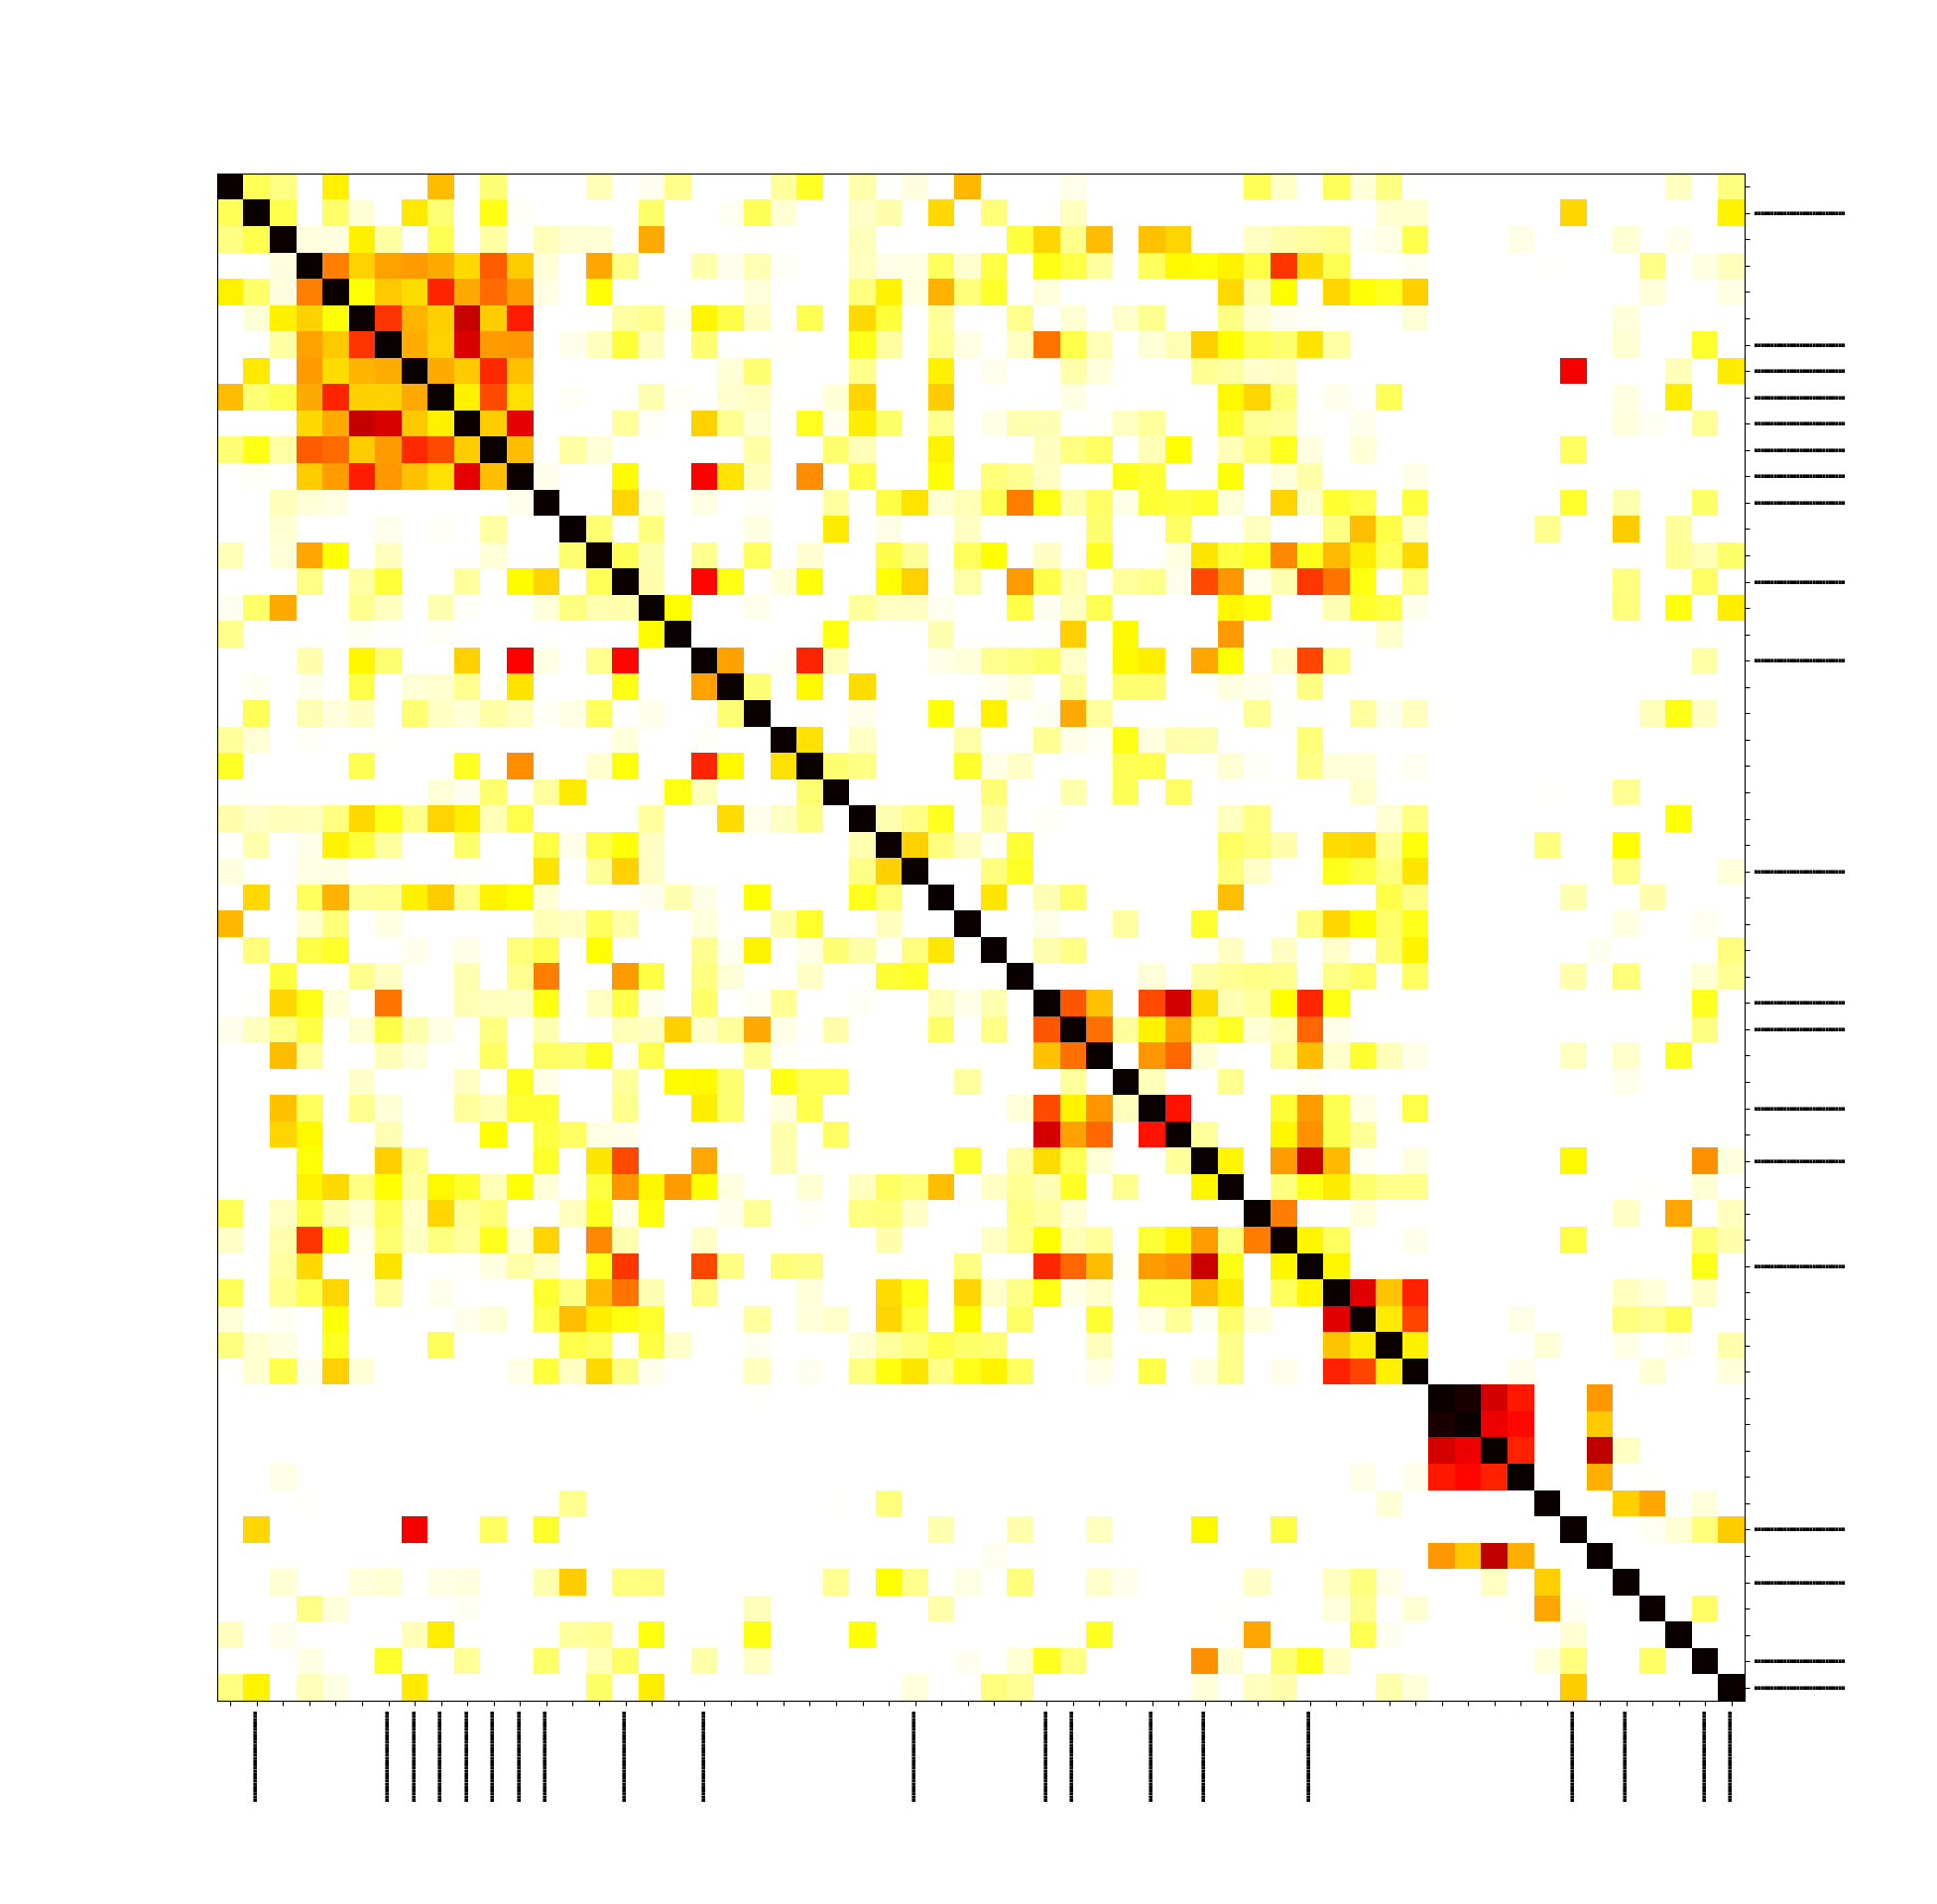
\includegraphics[width=\columnwidth]{zcash-mainnet-1543922496-fig-corr-005-txcl-003-N-Rand.png}
		\caption{Coinomi (Zcash)}
	\end{subfigure}
	\caption[short]{Experimental results (Bitcoin unless specified)}
	\label{fig:clustering-all}
\end{figure}

We performed experiments on Bitcoin testnet (Bitcoin wallet), Bitcoin mainnet (Bitcoin wallet, BRD, Coinomi, Mycelium), and Zcash (Coinomi).
Bitcoin wallet and BRD use P2P broadcast; Coinomi and Mycelium use centralized broadcast.
Experiments on testnet allow us to establish the upper bound on the effectiveness of our approach, as the testnet has a lower transaction rate and fewer nodes, which allows us to occupy all available connection slots.
We considered the number of first propagations in the range from 3 to 7, $k = 5$.
%We tried to connect to all peers with a maximum of 117~connections (established around 60~connections per node on average).
%Bitcoin wallet and BRD are the two most popular~\cite{Wang_TowardsBetterUnderstanding} mobile Bitcoin wallets.

The results are presented in Figure~\ref{fig:clustering-all}.
Our (control) transactions are marked with black ticks.
The color of each square represents the correlation coefficient between the weight vectors of two transactions (darker is higher).
As expected, the matrices exhibit a block-diagonal structure, with clusters along the main diagonal corresponding to transaction sources.
The clusters are clearly visible for the testnet version of Bitcoin wallet, we obtained a low (good for the attacker) anonymity degree of 0.5089.
The adjusted anonymity degree ($d_{adj}$) for Bitcoin wallet (mainnet) is 0.8646, BRD (mainnet) -- 0.8413, Coinomi -- 0.9117.
The experimental results show that while our technique shows the expected results on small networks, the picture for the Bitcoin mainnet is much less clear.
This may be explained by a much larger total number of nodes and transactions, and to the fact that we only run the experiment on a subset of Bitcoin nodes to avoid disrupting the network.

\subsubsection{Estimating the IP addresses of wallet's nodes}

Apart from clustering transactions, an adversary might be interested in obtaining the IP address of the nodes which a centralized wallet uses for transaction broadcast.
While the IP address of a centralized wallet's node may not necessarily be secret, the fact that a transaction from a particular Bitcoin address is propagated from such node may give an adversary a clue on which software the victim is using, which helps set up e.g. phishing or other social engineering attacks.
We test this attack scenario in the experiments on Mycelium (Bitcoin testnet) and Coinomi (Zcash).

Mycelium transactions cluster well: they are quickly propagated from the same two IP addresses (delay in single milliseconds), rebroadcasts from other nodes follow after tens or even hundreds of milliseconds.
According to IP geolocation services, these nodes are located in Germany (\texttt{2a01:4f9:2b:4ca::2}) and in Helsinki, Finland (\texttt{95.216.68.181}).
According to a reverse DNS lookup service \url{robtex.com}, one of these IP addresses corresponds to a URL~\url{electrumx-b.mycelium.com}.
Both addresses belong to Hetzner (a cloud provider), have an uptime of 2~months (at the time of writing), and a latency of 25~ms, as per Bitnodes~\cite{Bitnodes}.
In a separate experiment, we discovered that each of them has more than 700~slots.
%All these facts indicate that the nodes in question are related to business activity.
We discovered that there are also Bitcoin mainnet nodes running at the same IP addresses.
%Similar experiments on the mainnet did not reveal clear clustering due to factors we will discuss later.

% At the time of the experiment, Zcash has 176 live nodes, we connected to all of them with an average of 32~connections and captured 20~minuted of traffic.
In the Zcash experiment (Coinomi), though our transactions don't form a clear cluster, we observe that some of them (in the second cluster) were first received from the same IP (\texttt{5.79.123.194}), which, we assume, is at least one of the Coinomi's nodes.



\section{Attack cost estimation}

We now estimate the resources required for a full-scale attack on the Bitcoin mainnet.
As of November~2018, the Bitcoin mainnet consists of approximately 10\,000 nodes.
% 9887 90-day avg as of 2018-11-11
% https://bitnodes.earn.com/dashboard/?days=90
According to our measurements, the average number of free slots is 43 (measured on 1000~random peers).
According to the Bitcoin protocol documentation~\cite{BitcoinWiki}, the size of an INV message is "36x + const for message with x objects".
We assume an INV for a single transaction requires 40~bytes.
An average Bitcoin transaction rate, as of November~2018, is around 250\,000 transactions per day, or 2.89 tx/s.
Assuming each connection eventually relays each transaction, we arrive at the required bandwidth for one connection slot as: 2.89 tx/s * 40 b/tx = 115.6 b/s.
A full-scale attack on Bitcoin mainnet would require maintaining an average of 43~connections to 10\,000 nodes, i.e.,~ a total bandwidth of 115.6 b/s * 10000 nodes * 43 slots/node = 49708000 b/s = 47.4 Mb/s = 379 Mbit/s.
An hour-long attack at this bandwidth will require receiving approximately 167~GB of incoming traffic.

We may estimate the monetary cost of the attack based on the costs of running a Bitcoin full node on a cloud server.
Various estimations put that cost at between \$3 and \$20 per month~\cite{Zeyde2018, Connell2017}.
% "~3$ for the first year"
% $ 8.50 per calculator
% https://calculator.s3.amazonaws.com/index.html#r=IAD&s=EC2&key=calc-7C655B73-FA35-40F0-9518-4773E3E4A8C7
% "ran a Bitcoin node on Amazon Web Services for $20.43 per month"
% "a virtual private server for $5-10/month"
Bitcoin~Core maintains 8~outgoing and accepts up to 117~incoming connections by default.
In our measurements, an average Bitcoin server has 43~open slots.
Assuming it has a total of 125~slots, 125 - 43 = 82~slots eventually get occupied.
An adversary needs to maintain 10\,000 * 43 = 430\,000 connections, or 5244.0~times the bandwidth of a regular node.
A 30-days month is 720~hours.
Considering all of the above, we conclude that an estimated cost of an hour-long attack is approximately 5244 / 720 = 7.3~times the monthly cost of running a full node.
That leads to an estimation of bandwidth costs at \$20 -- 150.
Even taking into account the cost of computation and storage, the total cost of the attack is on the order of hundreds of US~dollars -- well within reach of even amateur adversaries, not to mention professional black-hat hackers and nation states.

All our experiments on Bitcoin testnet and Zcash mainnet cost \$35 (this can probably be decreased by optimizing the scripts, immediately copying the data to a local machine and deleting it from the cloud, etc).


\section{Discussion and countermeasures}

We now discuss the possible attack scenarios and countermeasures.

Experiments have shown that our approach works well in small networks (Bitcoin testnet, Zcash), but shows weaker results for Bitcoin mainnet.
Bitcoin mainnet, being substantially larger than alternative networks, requires significant resources just to capture the traffic.
Moreover, Bitcoin nodes have fewer free slots, and often limit the number of slots one IP can occupy.
These factors combined with a higher overall transaction rate makes clustering in Bitcoin harder.
Note also that we deliberately connected only to a small subset of the Bitcoin mainnet (up to 1000~out of approximately 10~thousand nodes) due to resource constraints.
A more resourceful attacker may achieve better results.
In addition, an adversary can use the testnet version of popular wallets to reveal information about the corresponding mainnet nodes (assuming both testnet and mainnet nodes are run on servers with related IP addresses).
The main limitation of our technique is the assumption that a user issues multiple transactions during a relatively short time frame through the same node.

Application-level cryptographic techniques, such as zero-knowledge proofs in Zcash, can not defend against our attack, as we only consider transaction hashes and their propagation times, ignoring their content.

A popular mitigation for deanonymization attacks based on network analysis is to use anonymity overlay networks such as Tor~\cite{Tor}, or mix networks such as Loopix~\cite{Piotrowska2017}.
In our case, this countermeasure is inefficient: transactions issued by the same cryptocurrency node can be linked by a global passive adversary even if the data was transferred through Tor or other anonymity network before being publicly broadcast.
Tor helps to hide the relationship between IP addresses of the originating node and the first node to broadcast the transaction to the peer-to-peer network, but we cluster transactions based on the first broadcaster's entry nodes (or nodes topologically close to those in terms of network propagation times), not the IP addresses of the originating node.
Note that broadcasting transactions via Tor may even introduce additional man-in-the-middle vulnerabilities~\cite{Biryukov2015} (the situation is similar to the case of a light wallet described below).

We distinguish three cases depending on the type of the user's wallet.

\paragraph{Full node with incoming connections (server)}
A typical operator of a Bitcoin server is either a business (wallet provider, exchange, etc), or an enthusiast willing to donate their computing resources to help the network.
In the first case, the transaction relayed through the node may originate from multiple users of this business, which also harms their privacy.
The full node operator may implement the following countermeasures:
\begin{itemize}
	\item Run the node with an increased number of outgoing connections to  dilute the quality of the topological fingerprint;
	\item Use additional random delays on top of those implemented in the node software;
	\item Drop connections to randomly chosen entry nodes and establish new ones, constantly altering the set of entry nodes;
	\item Give advice to users not to broadcast sensitive transactions within a short period of time.
\end{itemize}

\paragraph{Full node without incoming connections}
Transactions originating from a full node without incoming connections (ex. computer behind NAT) may be clustered based on the set of entry nodes.
In order to prevent that, the user can re-launch the software after making a transaction, so that each transaction would be broadcast through a new set of entry nodes.

\paragraph{Light wallets}
The majority of Bitcoin users use light wallets, i.e.,~they delegate validation to another full node using simple payment verification (SPV).
From the networking perspective, most light wallets, especially mobile ones, do not even connect to a P2P network.
Instead, they send transactions to the server of the wallet provider via TLS, which in turn broadcasts them to the P2P network.\footnote{Apart from clustering, this poses an arguably more serious privacy threat, which is outside the scope of this work: the wallet provider can log all users' transactions and link them to their IP addresses. Using Tor is not applicable in this case, as the wallet servers will still be able to associate a user's transactions by other means (e.g.,~by making the wallet send a cookie along with transactions).}
Proposed countermeasures for light wallets would be:
\begin{itemize}
	\item Use wallets that connect to the actual P2P network and broadcast transactions without relying on a centralized server (e.g.,~Bitcoin wallet for Android~\cite{BitcoinWallet});
	\item Use different light wallets for transactions not meant to be linkable;
	\item If the above advice is inapplicable, at least choose a popular light wallet to increase the anonymity set.
\end{itemize}

\paragraph{Mobile wallets}
There is an inherent trade-off between wallets with centralized and P2P broadcast.
Centralized wallets may better protect the user's privacy from external adversaries, but can themselves link users' transactions and correlate them with additional information obtained from the app.
Users must also trust centralized wallet providers for availability.
%If the wallet's server is down, the service is inaccessible, as happened with both Coinomi~\cite{CoinomiDownReddit} and Mycelium~\cite{MyceliumDownReddit}.
Wallets with P2P broadcast eliminate the danger of censorship, denial of service or deanonymization by the wallet provider, but reveal more information to an external observer.

Users of P2P wallets should connect to a trusted full node and avoid sending multiple transactions within a short time frame.
The best practices for secure coding are especially relevant for mobile wallets, which run on devices storing lots of personal data.
Wallet developers should use as few permissions as possible, open-source the code, provide alternative installation methods (F-Droid, direct APK download), and implement additional network-level measures to prevent traffic analysis.

An attacker may leverage additional information to increase clustering accuracy.
For instance, transactions issued by regular users usually contain a small number of inputs and two~outputs (destination and change).
Transactions with a large number of inputs or outputs are likely to have originated from a node associated with a business (a custodial wallet, an exchange, a mining pool).
An attacker trying to deanonymize a regular user can remove clusters with many "enterprise" transactions, making the victim's anonymity set smaller, and use known addresses of various services from sources like~\cite{Walletexplorer}.
We leave this research direction for future work.

\paragraph{Dandelion}

Dandelion~\cite{Venkatakrishnan2017} and its improvement Dandelion++~\cite{Fanti2018} are message propagation protocols for P2P networks designed to prevent deanonymization attacks.
Its key idea is introducing asymmetry: a message is first sent along a random path, and only then broadcast gossip-style.
Message propagation in Dandelion++\footnote{We focus on the latest, improved version of the protocol.} proceeds in two stages: the "stem" phase and the "fluff" stage.
In the stem phase, a new message is broadcast along a random path in the anonymity graph: an approximately regular random graph based on the same set of nodes as the regular P2P network.
In the fluff phase, the latest node to receive the message disperses it using the regular gossip-style broadcast.
The authors show that the protocol achieves much stronger anonymity than Bitcoin's current propagation mechanism, though at the cost of a several second propagation delay and additional sensitivity to DoS attacks at stem phase. 

Though the authors mention (Section~4.2) that some configurations of the protocol may be prone to transaction  correlation attacks, our approach is not suitable against Dandelion++.
The key feature that allows our well-connected listening node to gather useful information is that nodes choose neighbors to propagate messages at random, without distinguishing incoming and outgoing connections.
This means that by saturating 50\% of a node's connection slots we have a 50\% chance to be the first to receive a new transaction from it.
In Dandelion++, nodes choose neighbors for the stem phase propagation only from outgoing connections.
There is no obvious way to force a remote peer to initiate a connection to us, therefore a malicious node with many outgoing connections will not have any advantage in the stem phase (it can only aggregate incoming information while acting as a regular relay, which may gain some but not much insight into possible transaction clusters).


\section{Conclusion} \label{sec:Ch03Conclusion}

We study the state of anonymity of cryptocurrencies on the network level.
We describe and implement a novel kind of transaction clustering based on the analysis of propagation times.
We implement and test our tool on four popular cryptocurrencies: Bitcoin, Zcash, Dash, and Monero.
Our results indicate that many cryptocurrencies, including privacy-focused ones, do not sufficiently defend against our attack: a low budget adversary can link transactions initially broadcast from the same node with a high degree of accuracy.
The same set of tools allows an attacker to find out IP addresses of nodes which centralized wallets use for broadcasting transactions.
We argue that cryptocurrencies must defend against network analysis to provide stronger privacy guarantees.

Privacy-focused cryptocurrencies, while employing sophisticated cryptographic techniques to prevent blockchain analysis, are similar to Bitcoin on the network level.
Their lower overall popularity and a smaller anonymity set make them susceptible to network analysis.
A smaller number of privacy-friendly wallets exacerbate the threat.
We encourage privacy-conscious cryptocurrency users to choose their wallet according to privacy trade-offs.




